% !TEX encoding = UTF-8 Unicode

%\documentclass[b5paper]{book}

\newif\ifcrnobelo
%\crnobelotrue   %otkomentarisati za crno-belu varijantu

\newif\ifuboji
\ubojitrue       %zakomentarisati za crno-belu varijantu

\newif\ifrecenzija
%\recenzijatrue

\newif\ifstampanaverzija
\stampanaverzijatrue
%\stampanaverzijafalse

\ifstampanaverzija
\documentclass[pdftex,b5paper,twoside]{book}
\setlength{\textheight}{190mm}
\setlength{\topmargin}{0mm}
\fi

\ifrecenzija
\documentclass[a4paper]{book}
\setlength{\textheight}{280mm}
\setlength{\topmargin}{0mm}
\usepackage[lmargin=3.0cm, rmargin=3.0cm,tmargin=2.5cm,bmargin=2.50cm]{geometry}
\fi


\usepackage[T2A]{fontenc} % enable Cyrillic fonts
\usepackage[utf8x,utf8]{inputenc} % make weird characters work
%\usepackage[serbian]{babel}
%\usepackage[english,serbianc]{babel}
\usepackage[english,serbian]{babel}

%TODO: Izbaciti nepotrebne pakete

\usepackage{tikz}
\usepackage{color}
\usepackage{fancyhdr}
\usepackage{url}
\usepackage{caption}
\usepackage{amsmath}
\usepackage{amssymb}
\usepackage{setspace}
\usepackage{pdfpages}
\usepackage{longtable} 
\usepackage{wasysym}
\usepackage{pgf}
\usepackage{verbatim}
\usepackage{fancyvrb}

\usepackage{booktabs}
\usepackage[textfont=it]{caption}
\usepackage[margin=30mm]{geometry}
\usepackage{setspace}
\usepackage{pdfpages}

\usepackage{listings}

\usepackage[unicode]{hyperref}
%\hypersetup{colorlinks,citecolor=black,filecolor=black,linkcolor=black,urlcolor=black}
\hypersetup{colorlinks,citecolor=green,filecolor=green,linkcolor=blue,urlcolor=blue}

\usepackage[answerdelayed,lastexercise]{exercise}



\def\chaptername{}
\def\bibname{Literatura}
\def\appendixname{Dodatak}

\usepackage{lipsum}
\newcommand*\justify{%
  \fontdimen2\font=0.4em% interword space
  \fontdimen3\font=0.2em% interword stretch
  \fontdimen4\font=0.1em% interword shrink
  \fontdimen7\font=0.1em% extra space
  \hyphenchar\font=`\-% allowing hyphenation
}


\newcommand\estrana{\ifelektronskaverzija \newpage \fi}
\newcommand\skrati[1]{\ifpdf \else \vspace*{-#1mm} \fi}
\newcommand\kckod[1]{\texttt{\justify #1}}        % kratak c kod
\newcommand\argf[1]{\texttt{#1}}         % argument funkcije
\newcommand\komentar[1]{\textcolor{red}{#1}}         % komentar

\numberwithin{Answer}{chapter}
\numberwithin{Exercise}{chapter}

%Detalji se mogu naci na
%https://en.wikibooks.org/wiki/LaTeX/Source_Code_Listings

\ifcrnobelo
%https://en.wikibooks.org/wiki/LaTeX/Source_Code_Listings
\lstset{ 
backgroundcolor=\color{white},   % choose the background color; you must add \usepackage{color} or \usepackage{xcolor}
 basicstyle=\footnotesize,        % the size of the fonts that are used for the code
 breakatwhitespace=false,         % sets if automatic breaks should only happen at whitespace
 breaklines=true,                 % sets automatic line breaking
% captionpos=t,                    % sets the caption-position to bottom
 commentstyle=\color{black},    % comment style
 escapeinside={\%*}{*)},          % if you want to add LaTeX within your code
 extendedchars=true,              % lets you use non-ASCII characters; for 8-bits encodings only, does not work with UTF-8
 frame=single,	                   % adds a frame around the code
 keepspaces=true,                 % keeps spaces in text, useful for keeping indentation of code (possibly needs columns=flexible)
 keywordstyle=\color{black},       % keyword style
 language=C,                 % the language of the code
 numbers=left,                    % where to put the line-numbers; possible values are (none, left, right)
 numbersep=5pt,                   % how far the line-numbers are from the code
 numberstyle=\tiny\color{black}, % the style that is used for the line-numbers
 rulecolor=\color{black},         % if not set, the frame-color may be changed on line-breaks within not-black text (e.g. comments (green here))
 showspaces=false,                % show spaces everywhere adding particular underscores; it overrides 'showstringspaces'
 showstringspaces=false,          % underline spaces within strings only
 showtabs=false,                  % show tabs within strings adding particular underscores
 stepnumber=2,                    % the step between two line-numbers. If it's 1, each line will be numbered
 stringstyle=\color{black},     % string literal style
 tabsize=2,	                   % sets default tabsize to 2 spaces
}

%\renewcommand{\lstlistingname}{Datoteka}

\lstdefinestyle{customc}{
 belowcaptionskip=1\baselineskip,
 breaklines=true,
 xleftmargin=\parindent,
 language=C,
 basicstyle=\scriptsize,        % the size of the fonts that are used for the code
 showstringspaces=false,
 commentstyle=\color{black}\ttfamily,
 morecomment=[l][\color{black}]{\#},
 basicstyle=\footnotesize\ttfamily,
 keywordstyle=\bfseries\color{black}\ttfamily\textbf,
 identifierstyle=\bfseries\color{black}\ttfamily,
 stringstyle=\bfseries\color{black}\ttfamily,
% title={Program: \texttt{\lstname}},
}
\fi


\ifuboji

\definecolor{mygreen}{rgb}{0,0.6,0} 
\definecolor{mygray}{rgb}{0.5,0.5,0.5} 
\definecolor{mymauve}{rgb}{0.58,0,0.82}

%https://en.wikibooks.org/wiki/LaTeX/Source_Code_Listings
\lstset{ 
backgroundcolor=\color{white},   % choose the background color; you must add \usepackage{color} or \usepackage{xcolor}
 basicstyle=\footnotesize,        % the size of the fonts that are used for the code
 breakatwhitespace=false,         % sets if automatic breaks should only happen at whitespace
 breaklines=true,                 % sets automatic line breaking
% captionpos=t,                    % sets the caption-position to bottom
 commentstyle=\color{mygreen},    % comment style
 escapeinside={\%*}{*)},          % if you want to add LaTeX within your code
 extendedchars=true,              % lets you use non-ASCII characters; for 8-bits encodings only, does not work with UTF-8
 frame=single,	                   % adds a frame around the code
 keepspaces=true,                 % keeps spaces in text, useful for keeping indentation of code (possibly needs columns=flexible)
 keywordstyle=\color{blue},       % keyword style
 language=C,                 % the language of the code
 numbers=left,                    % where to put the line-numbers; possible values are (none, left, right)
 numbersep=5pt,                   % how far the line-numbers are from the code
 numberstyle=\tiny\color{mygray}, % the style that is used for the line-numbers
 rulecolor=\color{black},         % if not set, the frame-color may be changed on line-breaks within not-black text (e.g. comments (green here))
 showspaces=false,                % show spaces everywhere adding particular underscores; it overrides 'showstringspaces'
 showstringspaces=false,          % underline spaces within strings only
 showtabs=false,                  % show tabs within strings adding particular underscores
 stepnumber=2,                    % the step between two line-numbers. If it's 1, each line will be numbered
 stringstyle=\color{mymauve},     % string literal style
 tabsize=2,	                   % sets default tabsize to 2 spaces
}

%\renewcommand{\lstlistingname}{Datoteka}

\lstdefinestyle{customc}{
 belowcaptionskip=1\baselineskip,
 breaklines=true,
 xleftmargin=\parindent,
 language=C,
 basicstyle=\scriptsize,        % the size of the fonts that are used for the code
 showstringspaces=false,
 commentstyle=\color{blue}\ttfamily,
 morecomment=[l][\color{magenta}]{\#},
 basicstyle=\footnotesize\ttfamily,
 keywordstyle=\bfseries\color{green!40!black}\ttfamily\textbf,
 identifierstyle=\bfseries\color{black}\ttfamily,
 stringstyle=\bfseries\color{magenta}\ttfamily,
% title={Program: \texttt{\lstname}},
}
\fi

\newcommand{\includecodeLib}[2]{\lstinputlisting[title=#2,language=C,style=customc]{#1}}
\newcommand{\includecode}[1]{\lstinputlisting[language=C,style=customc]{#1}}

%\def\d{{\fontencoding{T1}\selectfont\dj}}
%\def\D{{\fontencoding{T1}\selectfont\DJ}}

\lstset{literate=
 {č}{{\v{c}}}1 {ć}{{\'{c}}}1 {š}{{\v{s}}}1 {ž}{{\v{z}}}1 {đ}{{\d}}1 
 {Č}{{\v{C}}}1 {Ć}{{\'{C}}}1 {Š}{{\v{S}}}1 {Ž}{{\v{Z}}}1 {Đ}{{\D}}1  
}


\newcommand{\uputstvo}[1]{\textsc{Uputstvo:} \emph{#1}}
\newcommand{\napomena}[1]{\textsc{Napomena:} \emph{#1}}
\newcommand{\linkresenje}[1]{\ifpdf \flushright [Rešenje \refAnswer{#1}] \fi}

\newenvironment{ckod}
{\verbatim}
{\endverbatim}



\ifcrnobelo
\newcommand{\datoteka}[1]{\textcolor{black}{\texttt{\hspace{2mm}#1}}}
\newcommand{\poziv}[1]{\textcolor{black}{\textsc{Pokretanje:\hspace{2mm}}}#1}
\newcommand{\ulaz}[1]{\textcolor{black}{\texttt{\textit{\hspace{2mm}#1}}}}
\newcommand{\izlaz}[1]{\textcolor{black}{\texttt{\hspace{2mm}#1}}}
\newcommand{\naslovInt}{\textcolor{black}{\textsc{Interakcija sa programom:}}}
\newcommand{\naslovDat}[1]{\textcolor{black}{\textsc{#1}}}
\newcommand{\naslovUlaz}{\textcolor{black}{\textsc{Ulaz:}}}
\newcommand{\naslovIzlaz}{\textcolor{black}{\textsc{Izlaz:}}}
\newcommand{\naslovIzlazZaGresku}{\textcolor{black}{\textsc{Izlaz za gre\v{s}ke:}}}

\lstnewenvironment{upotreba}[1]
{
 \renewcommand\lstlistingname{Test}\lstset{
% belowcaptionskip=1\baselineskip,
% breaklines=true,
 frame=L,
 backgroundcolor=\color{white},
% xleftmargin=\parindent,
 language=C,
 showstringspaces=false,
 basicstyle=\scriptsize\ttfamily,
 keywordstyle=\bfseries\color{black},
 commentstyle=\itshape\color{black},
 identifierstyle=\color{black},
 stringstyle=\color{black},
 numbers=none,
 captionpos=t,
 title={Primer #1},
 escapechar={\#}
}
}
{}


\lstnewenvironment{test}[1]
{
 \renewcommand\lstlistingname{Test}\lstset{
% belowcaptionskip=1\baselineskip,
% breaklines=true,
 frame=L,
 backgroundcolor=\color{white},
% xleftmargin=\parindent,
 language=C,
 showstringspaces=false,
 basicstyle=\scriptsize\ttfamily,
 keywordstyle=\bfseries\color{black},
 commentstyle=\itshape\color{black},
 identifierstyle=\color{black},
 stringstyle=\color{black},
 numbers=none,
 captionpos=t,
 title={Test #1},
 escapechar={\#}
}
}
{}

\lstnewenvironment{test2}[1]
{
 \renewcommand\lstlistingname{Test}\lstset{
% belowcaptionskip=1\baselineskip,
% breaklines=true,
 frame=no,
 backgroundcolor=\color{white},
% xleftmargin=\parindent,
 language=C,
 showstringspaces=false,
 basicstyle=\scriptsize\ttfamily,
 keywordstyle=\bfseries\color{black},
 commentstyle=\itshape\color{black},
 identifierstyle=\color{black},
 stringstyle=\color{black},
 numbers=none,
 captionpos=t,
% title={Test #1},
 escapechar={\#}
}
}
{}
\fi




%http://latexcolor.com/

\ifuboji
\definecolor{dmg}{rgb}{0.05, 0.5, 0.06}
\definecolor{djg}{rgb}{0.0, 0.29, 0.29}
\definecolor{denim}{rgb}{0.08, 0.38, 0.74}
\definecolor{egyptianblue}{rgb}{0.06, 0.2, 0.65}

\newcommand{\datoteka}[1]{\textcolor{dmg}{\texttt{\hspace{2mm}#1}}}
\newcommand{\poziv}[1]{\textcolor{dmg}{\textsc{Pokretanje:\hspace{2mm}}}#1}
\newcommand{\ulaz}[1]{\textcolor{black}{\texttt{\textit{\hspace{2mm}#1}}}}
\newcommand{\izlaz}[1]{\textcolor{blue}{\texttt{\hspace{2mm}#1}}}
\newcommand{\naslovInt}{\textcolor{egyptianblue}{\textsc{Interakcija sa programom:}}}
\newcommand{\naslovDat}[1]{\textcolor{djg}{\textsc{#1}}}
\newcommand{\naslovUlaz}{\textcolor{egyptianblue}{\textsc{Ulaz:}}}
\newcommand{\naslovIzlaz}{\textcolor{egyptianblue}{\textsc{Izlaz:}}}
\newcommand{\naslovIzlazZaGresku}{\textcolor{egyptianblue}{\textsc{Izlaz za gre\v{s}ke:}}}

\lstnewenvironment{upotreba}[1]
{
 \renewcommand\lstlistingname{Test}\lstset{
% belowcaptionskip=1\baselineskip,
% breaklines=true,
 frame=L,
 backgroundcolor=\color{white},
% xleftmargin=\parindent,
 language=C,
 showstringspaces=false,
 basicstyle=\scriptsize\ttfamily,
 keywordstyle=\bfseries\color{green!40!black},
 commentstyle=\itshape\color{purple!40!black},
 identifierstyle=\color{blue},
 stringstyle=\color{orange},
 numbers=none,
 captionpos=t,
 title={Primer #1},
 escapechar={\#}
}
}
{}


\lstnewenvironment{test}[1]
{
 \renewcommand\lstlistingname{Test}\lstset{
% belowcaptionskip=1\baselineskip,
% breaklines=true,
 frame=L,
 backgroundcolor=\color{white},
% xleftmargin=\parindent,
 language=C,
 showstringspaces=false,
 basicstyle=\scriptsize\ttfamily,
 keywordstyle=\bfseries\color{green!40!black},
 commentstyle=\itshape\color{purple!40!black},
 identifierstyle=\color{blue},
 stringstyle=\color{orange},
 numbers=none,
 captionpos=t,
 title={Test #1},
 escapechar={\#}
}
}
{}

\lstnewenvironment{test2}[1]
{
 \renewcommand\lstlistingname{Test}\lstset{
% belowcaptionskip=1\baselineskip,
% breaklines=true,
 frame=no,
 backgroundcolor=\color{white},
% xleftmargin=\parindent,
 language=C,
 showstringspaces=false,
 basicstyle=\scriptsize\ttfamily,
 keywordstyle=\bfseries\color{green!40!black},
 commentstyle=\itshape\color{purple!40!black},
 identifierstyle=\color{blue},
 stringstyle=\color{orange},
 numbers=none,
 captionpos=t,
% title={Test #1},
 escapechar={\#}
}
}
{}
\fi

\usepackage{caption}
\DeclareCaptionFormat{listing} {
  \parbox[top][10pt][l]{\textwidth}{\hspace{0pt}#1#2#3}
}
\captionsetup[lstlisting]{format=listing, font={small,tt}}

\newenvironment{minitest}
{\begin{minipage}[t]{40mm}} 
{\end{minipage}}

\newenvironment{miditest}
{\begin{minipage}[t]{65mm}}
{\end{minipage}}

\newenvironment{maxitest}
{\begin{minipage}[t]{150mm}}
{\end{minipage}}


\def\ExerciseName{Zadatak }
\def\AnswerName{Rešenje }

\def\DifficultyMarker{*}

\renewcommand{\ExerciseHeader}{{\textbf{
\ExerciseHeaderDifficulty \ExerciseName \ExerciseHeaderNB \ExerciseHeaderTitle 
\ExerciseHeaderOrigin}}}

\renewcommand{\AnswerHeader}{{\textbf{
\AnswerName \ExerciseHeaderNB \ExerciseHeaderTitle
\medskip}}}


\RecustomVerbatimCommand{\VerbatimInput}{VerbatimInput}%
{fontsize=\footnotesize,
 %
 frame=lines,  % top and bottom rule only
 framesep=1em, % separation between frame and text
 rulecolor=\color{gray},
 %
% label=\fbox{\color{black}data.txt},
% labelposition=topline,
 %
% commandchars=\|\(\), % escape character and argument delimiters for
                      % commands within the verbatim
 commentchar=*        % comment character
}


\setenumerate[0]{label=(\alph*)}
\hyphenation{Kom-pleks-anBroj}
\hyphenation{ko-ja}
\hyphenation{prebroj-_-bitove}
\hyphenation{adresa-_-glave}
\hyphenation{he-ap}




\newif\ifpdf
\pdftrue       %postaviti na false za izbacivanje linkova na resenja
\usepackage{fancyhdr}

\begin{document}
\pagenumbering{roman}

\pagestyle{empty}

\begin{center}
{\sffamily

{\fontsize{16pt}{19pt}\selectfont Univerzitet u Beogradu}

{\fontsize{16pt}{19pt}\selectfont Matematički fakultet}
\vspace{70pt}

{\fontsize{16pt}{19pt}\selectfont \bfseries  Milena Vujošević Janičić, Jelena Graovac, Ana Spasić, Mirko Spasić, Anđelka Zečević, Nina Radojičić}

\vspace{50pt}
%{\fontsize{22pt}{26pt}\selectfont {Programiranje 2 \\ Zbirka zadataka sa rešenjima}}
\centerline{{\huge\bfseries PROGRAMIRANJE 2}}
\centerline{{\huge\bfseries {\fontsize{22pt}{26pt}\selectfont {Zbirka zadataka sa rešenjima}}}}


\vspace{120pt}

\centerline{{\Large \bfseries Beograd}}
\centerline{{\Large \bfseries 2015.}}

%{\fontsize{14pt}{17pt}\selectfont Beograd, 2015.}
}
\end{center}



\newpage
\normalsize

\noindent
Autori: 

\noindent
{\slshape dr Milena Vujošević Janičić}, docent na Matematičkom fakultetu u Beogradu

\noindent
{\slshape dr Jelena Graovac}, docent na Matematičkom fakultetu u Beogradu

\noindent
{\slshape Ana Spasić}, asistent na Matematičkom fakultetu u Beogradu

\noindent
{\slshape Mirko Spasić}, asistent na Matematičkom fakultetu u Beogradu

\noindent
{\slshape Anđelka Zečević}, asistent na Matematičkom fakultetu u Beogradu

\noindent
{\slshape Nina Radojičić}, asistent na Matematičkom fakultetu u Beogradu
\vspace*{2mm}

\noindent
PROGRAMIRANJE 2\\
Zbirka zadataka sa rešenjima
\vspace*{3mm}


\noindent
Izdava\v{c}: Matematički fakultet Univerziteta u Beogradu

Studentski trg 16, 11000 Beograd

\noindent
Za izdava\v{c}a: {\slshape prof.~dr Zoran Rakić}, dekan
\vspace*{3mm}

\noindent
Recenzenti:

\noindent
{\slshape dr Gordana Pavlović-Lažetić}, redovni profesor na Matematičkom fakultetu u Beogradu

\noindent
{\slshape dr Mladen Nikolić}, docent na Matematičkom fakultetu u Beogradu

\noindent
{\slshape dr Dragan Urošević}, naučni savetnik na Matematičkom institutu SANU
\vspace*{3mm}

\noindent
Obrada teksta, crteži i korice: {\slshape autori}


\ifstampanaverzija
\noindent
Štampa: %Skripta internacional, Beograd 

\noindent
Tiraž: %100
\vspace*{3mm}


\font\cyr=wncyr10

\ifstampanaverzija

\noindent
CIP {\cyr Katalogizacija u publikaciji} 

\noindent
{\cyr Narodna biblioteka Srbije, Beograd}
\vspace*{1mm}

\else 
  \noindent ISBN XXX-XX-XXXX-XXX-X \vspace*{1cm}
\fi



\noindent
\copyright 2015. Milena Vujošević Janičić, Jelena Graovac, Ana Spasić, Mirko Spasić, Anđelka Zečević, Nina Radojičić


\noindent {\small Ovo delo zaštićeno je licencom Creative Commons
  CC BY-NC-ND 4.0 (Attribution-NonCommercial-NoDerivatives 4.0 International License). 
  Detalji licence mogu se videti na veb-adresi \url{http://creativecommons.org/licenses/by-nc-nd/4.0/}.
  Do\-zvo\-lje\-no je umnožavanje, distribucija i javno saopštavanje dela, pod uslovom da 
  se navedu imena autora. Upotreba dela u komercijalne svrhe nije dozvoljena. 
  Prerada, preoblikovanje i upotreba dela u sklopu nekog drugog nije dozvoljena.  }

\vspace*{1mm}
\noindent
\includegraphics[width=2.5cm]{cc.png}

\newpage


\tableofcontents


\chapter*{Predgovor}

U okviru kursa {\em Programiranje 2} na Matematičkom fakultetu vežbaju se zadaci 
koji imaju za cilj da studente nauče rekurzivnom pristupu rešavanju problema, 
ispravnom radu sa pokazivačima i dinamički alociranom memorijom, osnovnim algoritmima 
pretraživanja i sortiranja, kao i radu sa dinamičkim strukturama podataka, 
poput listi i stabala. Zadaci koji se nalaze u ovoj zbirci predstavljaju 
objedinjen skup zadataka sa vežbi i praktikuma ovog kursa, kao i primere 
zadataka sa održanih ispita. Elektronska verzija zbirke, dostupna je 
(besplatno) u okviru strane kursa \url{www.programiranje2.matf.bg.ac.rs}, 
a tu je dostupan i radni repozitorijum elektronskih verzija rešenja zadataka.

U prvom poglavlju zbirke obrađene su uvodne teme koje obuhvataju osnovne tehnike koje se koriste u rešavanju svih ostalih zadataka u zbirci: podela koda po datotekama i rekurzivni pristup rešvanju problema. Takođe, u okviru ovog poglavlja dati su i osnovni algoritmi za rad sa bitovima. Drugo poglavlje je posvećeno pokazivačima: pokazivačkoj aritmetici, višedimenzionim nizovima, dinamičkoj alokaciji memorije i radu sa pokazivačima na funkcije. Treće poglavlje obrađuje algoritme pretrage i sortiranja, a četvrto dinamičke strukture podataka: liste i stabla. Dodatak sadrži najvažnije ispitne rokove iz jedne akademske godine. Većina zdataka je rešena, a teži zadaci su obeleženi zvezdicom.


Autori velikog broja zadataka ove zbirke su ujedno i autori same zbirke, ali postoje 
i zadaci za koje se ne može tačno utvrditi ko je originalni autor jer su zadacima 
davali svoje doprinose različiti asistenti koji su držali vežbe iz ovog kursa u 
prethodnih desetak godina. Zbog toga smatramo da je naš osnovni doprinos 
što smo objedinili, precizno formulisali, rešili i detaljno iskomentarisali 
sve najvažnije zadatke koji su potrebni za uspešno savlađivanje koncepata 
koji se obrađuju u okviru kursa. 

\newpage
Zahvaljujemo recenzentima, Gordani Pavlović Lažetić i Draganu Uroševiću, na veoma pažljivom čitanju rukopisa i na brojnim korisnim sugestijama. Takođe, zahvaljujemo studentima koji su svojim aktivnim učešćem u nastavi pomogli i doprineli u obličavanju ovog materijala. 

Svi komentari i sugestije na zadatke i rešenja zbirke su dobrodošli i osećajte se slobodno da ih pošaljete elektronskom poštom bilo kome od autora\footnote{Adrese autora su: \texttt{milena}, \texttt{jgraovac}, \texttt{aspasic}, \texttt{mirko}, \texttt{andjelkaz}, \texttt{nina}, sa nastavkom \texttt{@matf.bg.ac.rs}}. 



%Da dodamo ko je radio na kom poglavlju?


\bigskip

\begin{flushright}
{\em Autori}
\end{flushright}


\def\chaptername{}

\renewcommand{\chaptermark}[1]{\markboth{\thechapter\ #1}{#1}}
\renewcommand{\sectionmark}[1]{\markright{\thesection\ #1}}

\chapter{Uvodni zadaci}


\iffalse
\pagestyle{fancy}
\fancyhf{}
\fancyhead[RE]{\bfseries\slshape\leftmark}
\fancyhead[LO]{\bfseries\slshape\rightmark}
\fancyfoot[RO,LE]{\thepage}
\fi

\pagestyle{fancyplain}
\renewcommand{\chaptermark}[1]{\markboth{\thechapter\ #1}{#1}}
\renewcommand{\sectionmark}[1]{\markright{\thesection\ #1}}
%\lhead[\fancyplain{}{\bfseries\slshape\thepage}]{\fancyplain{}{\bfseries\slshape\rightmark}}
%\rhead[\fancyplain{}{\bfseries\slshape\leftmark}]{\fancyplain{}{\bfseries\slshape\thepage }}
\lhead[\fancyplain{}{\bfseries\slshape\leftmark}]{\fancyplain{}{}}
\rhead[\fancyplain{}{}]{{\fancyplain{}{\bfseries\slshape\rightmark}}}
%\rhead[]{\fancyplain{}{\bfseries\slshape\rightmark}}
%\lhead[]{\fancyplain{}{\bfseries\slshape\leftmark}}
\cfoot{}

%\fancyhead[LE,RO]{\fancyplain{}{\bfseries\slshape\rightmark}
%\fancyhead[RE,LO]{\fancyplain{}{\bfseries\slshape\leftmark}}
\fancyfoot[LE]{\thepage} 
\fancyfoot[RO]{\thepage} 
 

\pagenumbering{arabic}
\setcounter{page}{1}


\section{Podela koda po datotekama}

\begin{Exercise}[label=1_01] % I sa vezbi
Napisati program za rad sa kompleksnim brojevima.
\begin{enumerate}
\item Definisati strukturu \kckod{KompleksanBroj} koja opisuje kompleksan broj zadat njegovim realnim i imaginarnim delom.
\item Napisati funkciju \kckod{void ucitaj\_kompleksan\_broj(KompleksanBroj * z)} koja učitava kompleksan broj \kckod{z} sa standardnog ulaza.
\item Napisati funkciju \kckod{void ispisi\_kompleksan\_broj(KompleksanBroj z)} koja ispisuje kompleksan broj \kckod{z} na standardni izlaz u odgovarajućem formatu. 
%(npr. broj čiji je realni deo \argf{2}, a imaginarni \argf{-3} treba ispisati kao $(2 - 3 i)$).
\item Napisati funkciju \kckod{float realan\_deo(KompleksanBroj z)} koja vraća vrednost realnog dela broja \kckod{z}.
\item Napisati funkciju \kckod{float imaginaran\_deo(KompleksanBroj z)} koja vraća vrednost imaginarnog dela broja \kckod{z}.
\item Napisati funkciju \kckod{float moduo(KompleksanBroj z)} koja vraća moduo kompleksnog broja \kckod{z}.
\item Napisati funkciju \kckod{KompleksanBroj konjugovan(KompleksanBroj z)} koja vraća konjugovano-kompleksni broj broja \kckod{z}.
\item Napisati funkciju \kckod{KompleksanBroj saberi(KompleksanBroj z1, KompleksanBroj z2)} koja vraća zbir dva kompleksna broja \kckod{z1} i \kckod{z2}.
\item Napisati funkciju \kckod{KompleksanBroj oduzmi(KompleksanBroj z1, KompleksanBroj z2)} koja vraća razliku dva kompleksna broja \kckod{z1} i \kckod{z2}.
\item Napisati funkciju \kckod{KompleksanBroj mnozi(KompleksanBroj z1, KompleksanBroj z2)} koja vraća proizvod dva kompleksna broja \kckod{z1} i \kckod{z2}.
\item Napisati funkciju \kckod{float argument(KompleksanBroj z)} koja vraća argument kompleksnog broja \kckod{z}.
\end{enumerate}

Napisati program koji testira prethodno napisane funkcije. Sa standardnog ulaza uneti dva kompleksna broja $z1$ i $z2$, a zatim ispisati realni deo, imaginarni deo, moduo, konjugovano-kompleksan broj i argument broja koji se dobija kao zbir, razlika ili proizvod brojeva $z1$ i $z2$ u zavisnosti od znaka ('+', '-', '*') koji se unosi sa standardnog ulaza. 

\begin{maxitest}
\begin{upotreba}{1}
#\naslovInt#
#\izlaz{Unesite realni i imaginarni deo kompleksnog broja:} \ulaz{1 -3}#
#\izlaz{(1.00 - 3.00 i)}#
#\izlaz{Unesite realni i imaginarni deo kompleksnog broja:} \ulaz{-1 4}#
#\izlaz{(-1.00 + 4.00 i)}#
#\izlaz{Unesite znak (+,-,*):} \ulaz{-}#
#\izlaz{(1.00 - 3.00 i) - (-1.00 + 4.00 i)  =  (2.00 - 7.00 i)}#
#\izlaz{Realni\_deo: 2}#
#\izlaz{Imaginarni\_deo: -7.000000}#
#\izlaz{Moduo: 7.280110}#
#\izlaz{Konjugovano kompleksan broj: (2.00 + 7.00 i)}#
#\izlaz{Argument kompleksnog broja: - 1.292497}#
\end{upotreba}
\end{maxitest}


\linkresenje{1_01}
\end{Exercise}
\begin{Answer}[ref=1_01]
\includecode{resenja/1_UvodniZadaci/1_01.c}
\end{Answer}

\begin{Exercise}[label=1_02] % III sa vezbi
Uraditi prethodni zadatak tako da su sve napisane funkcije za rad sa kompleksnim brojevima zajedno sa definicijom strukture \kckod{KompleksanBroj} izdvojene u posebnu biblioteku. Napisati program koji testira ovu biblioteku. Sa standardnog ulaza uneti kompeksan broj, a zatim na standardni izlaz ispisati njegov polarni oblik. 

\begin{maxitest}
\begin{upotreba}{1}
#\naslovInt#
#\izlaz{Unesite realni i imaginarni deo kompleksnog broja:} \ulaz{-5 2 }#
#\izlaz{Polarni oblik kompleksnog broja je 5.39 *  e\^{}i * 2.76}#
\end{upotreba}
\end{maxitest}

\linkresenje{1_02}

\end{Exercise}
\begin{Answer}[ref=1_02]
\includecodeLib{resenja/biblioteke/kompleksan_broj/kompleksan_broj.h}{kompleksan\_broj.h} 
\includecodeLib{resenja/biblioteke/kompleksan_broj/kompleksan_broj.c}{kompleksan\_broj.c}
\includecodeLib{resenja/1_UvodniZadaci/1_02.c}{main.c}
\end{Answer}


\begin{Exercise}[label=1_03] % sa praktikuma
Napisati biblioteku za rad sa polinomima.
  \begin{enumerate}
  \item Definisati strukturu \kckod{Polinom} koja opisuje polinom stepena najviše 20 koji je zadat nizom svojih koeficijenata tako da se na i-toj poziciji u nizu nalazi koeficijent uz i-ti stepen polinoma.
  \item Napisati funkciju \kckod{void ispisi(const Polinom * p)} koja ispisuje polinom \kckod{p} na standardni izlaz, od najvišeg ka najnižem stepenu. Ipisati samo koeficijente koji su različiti od nule.
  \item Napisati funkciju \kckod{Polinom ucitaj()} koja učitava polinom sa standardnog
    ulaza. Za polinom najpre uneti stepen, a zatim njegove koeficijente.
  \item Napisati funkciju \kckod{double izracunaj(const Polinom * p, double x)} koja vraća vrednosti polinoma \kckod{p} u
    datoj tački \kckod{x} koristeći Hornerov algoritam.
  \item Napisati funkciju \kckod{Polinom saberi(const Polinom * p, const Polinom * q)} koja vraća zbir dva polinoma \kckod{p} i \kckod{q}.
  \item Napisati funkciju \kckod{Polinom pomnozi(const Polinom * p, const Polinom * q)} koja vraća proizvod dva polinoma \kckod{p} i \kckod{q}.
  \item Napisati funkciju \kckod{Polinom izvod(const Polinom * p)} koja vraća izvod polinoma \kckod{p}.
  \item Napisati funkciju \kckod{Polinom n\_izvod(const Polinom * p, int n)} koja vraća \kckod{n}-ti izvod polinoma \kckod{p}.
  \end{enumerate}

Napisati program koji testira prethodno napisane funkcije. Sa standardnog ulaza učitati polinome \argf{p} i \argf{q}, a zatim ih ispisati na standardni izlaz u odgovarajućem formatu. Izračunati i ispisati zbir \argf{z} i proizvod \argf{r} unetih polinoma \argf{p} i \argf{q}. Sa standardnog ulaza učitati realni broj \argf{x}, a zatim na standardni izlaz ispisati vrednost polinoma \argf{z} u tački \argf{x} zaokruženu na dve decimale. Na kraju, sa standardnog ulaza učitati broj \argf{n} i na izlaz ispisati \argf{n}-ti izvod polinoma \argf{r}.

\begin{maxitest}
\begin{upotreba}{1}
#\naslovInt#
#\izlaz{Unesite polinom p (prvo stepen, pa zatim koeficijente od najveceg stepena do nultog):}#
#\ulaz{3 1.2 3.5 2.1 4.2}#
#\izlaz{Unesite polinom q (prvo stepen, pa zatim koeficijente od najveceg stepena do nultog):}#
#\ulaz{2 2.1 0 -3.9}#
#\izlaz{Zbir polinoma je polinom z:}#
#\izlaz{1.20x\^{}3+5.60x\^{}2+2.10x+0.30}# 
#\izlaz{Prozvod polinoma je polinom r:}#
#\izlaz{2.52x\^{}5+7.35x\^{}4-0.27x\^{}3-4.83x\^{}2-8.19x-16.38}#
#\izlaz{Unesite tacku u kojoj racunate vrednost polinoma z:}#
#\ulaz{0}#
#\izlaz{Vrednost polinoma z u tacki 0.00 je 0.30}#
#\izlaz{Unesite izvod polinoma koji zelite:}#
#\ulaz{3}#
#\izlaz{3. izvod polinoma r je: 151.20x\^{}2+176.40x-1.62}#
\end{upotreba}
\end{maxitest}

\linkresenje{1_03}

\end{Exercise}
\begin{Answer}[ref=1_03]
\includecodeLib{resenja/biblioteke/polinom/polinom.h}{polinom.h} 
\includecodeLib{resenja/biblioteke/polinom/polinom.c}{polinom.c}
\includecodeLib{resenja/1_UvodniZadaci/1_03.c}{main.c}
%\includecode{resenja/1_UvodniZadaci/003/Makefile}
\end{Answer}

\ifpdf
\else \newpage
\fi

\begin{Exercise}[label=1_04] % sa praktikuma
Napisati biblioteku za rad sa razlomcima.
  \begin{enumerate}
  \item Definisati strukturu \kckod{Razlomak} koja opisuje razlomak.
  \item Napisati funkciju \kckod{Razlomak ucitaj()} za učitavanje razlomka.
  \item Napisati funkciju \kckod{void ispisi(const Razlomak * r)} koja ispisuje razlomak \argf{r}.
  \item Napisati funkciju \kckod{int brojilac(const Razlomak * r)} koja vraćaja brojilac razlomka \kckod{r}.
   \item Napisati funkciju \kckod{int imenilac(const Razlomak * r)} koja vraćaja imenilac razlomka \kckod{r}.
  \item Napisati funkciju \kckod{double realna\_vrednost(const Razlomak * r)} koja vraća odgovarajuću realnu vrednost razlomka \kckod{r}.
  \item Napisati funkciju  \kckod{double reciprocna\_vrednost(const Razlomak * r)} koja vraća recipročnu vrednost
    razlomka \kckod{r}.
  \item Napisati funkciju \kckod{Razlomak skrati(const Razlomak * r)} koja vraća skraćenu vrednost datog razlomka \kckod{r}.
  \item Napisati funkciju \kckod{Razlomak saberi(const Razlomak * r1, const Razlomak * r2)} koja vraća zbir dva razlomka \kckod{r1} i \kckod{r2}.
 \item Napisati funkciju \kckod{Razlomak oduzmi(const Razlomak * r1, const Razlomak * r2)} koja vraća razliku dva razlomka \kckod{r1} i \kckod{r2}.
 \item Napisati funkciju \kckod{Razlomak pomnozi(const Razlomak * r1, const Razlomak * r2)} koja vraća proizvod dva razlomka \kckod{r1} i \kckod{r2}.
 \item Napisati funkciju \kckod{Razlomak podeli(const Razlomak * r1, const Razlomak * r2)} koja vraća količnik dva razlomka \kckod{r1} i \kckod{r2}.
\end{enumerate}
Napisati program koji testira prethodne funkcije. Sa standardnog ulaza učitati dva razlomka \argf{r1} i \argf{r2}. Na standardni izlaz ispisati skraćene vrednosti zbira, razlike, proizvoda i količnika
razlomaka \argf{r1} i recipročne vrednosti razlomka \argf{r2}.

\begin{maxitest}
\begin{upotreba}{1}
#\naslovInt#
#\izlaz{Unesite imenilac i brojilac prvog razlomka:}\ulaz{1 2}#
#\izlaz{Unesite imenilac i brojilac drugog razlomka:}\ulaz{2 3}#
#\izlaz{1/2 + 3/2 = 2}#
#\izlaz{1/2 - 3/2 =  -1}#
#\izlaz{1/2 * 3/2 =  3/4}#
#\izlaz{1/2 / 3/2 =  1/3}#
\end{upotreba}
\end{maxitest}


%\linkresenje{1_04}

\end{Exercise}
%\begin{Answer}[ref=1_04]
%%\includecode{resenja/...}
%\end{Answer}

\section{Algoritmi za rad sa bitovima}

\begin{Exercise}[label=1_05] %ex 201 dvestajedan
Napisati biblioteku \kckod{stampanje\_bitova} za rad sa bitovima. Biblioteka treba da sadrži funkcije \kckod{stampanje\_bitova}, 
\kckod{stampanje\_bitova\_short} i \kckod{stampanje\_bitova\_char} za štampanje bitova u binarnom zapisu celog broja 
tipa \kckod{int}, \kckod{short} i \kckod{char}, koji se zadaje kao argument funkcije. 
Napisati program koji testira napisanu biblioteku. Sa standardnog ulaza učitati u heksadekadnom formatu cele brojeve tipa
\kckod{int}, \kckod{short} i \kckod{char} i na standardni izlaz ispisati njihovu binarnu reprezentaciju.

\skrati{5}
\begin{maxitest}
\begin{upotreba}{1}
#\naslovInt#
#\izlaz{Unesite broj tipa int: }\ulaz{0x4f4f4f4f}#
#\izlaz{Binarna reprezentacija: 01001111010011110100111101001111}#
#\izlaz{Unesite broj tipa short: }\ulaz{0x4f4f}#
#\izlaz{Binarna reprezentacija: 0100111101001111}#
#\izlaz{Unesite broj tipa char: }\ulaz{0x4f}#
#\izlaz{Binarna reprezentacija: 01001111}#
\end{upotreba}
\end{maxitest}

\linkresenje{1_05}
\end{Exercise}
\begin{Answer}[ref=1_05]
\includecodeLib{resenja/biblioteke/stampanje_bitova/stampanje_bitova.h}{stampanje\_bitova.h}
\includecodeLib{resenja/biblioteke/stampanje_bitova/stampanje_bitova.c}{stampanje\_bitova.c}
\includecodeLib{resenja/1_UvodniZadaci/1_05.c}{main.c}
\end{Answer}

\begin{Exercise}[label=1_06]
Napisati funkcije \kckod{\_bitove\_1} i \kckod{prebroj\_bitove\_2} koje vraćaju broj jedinica u 
binarnom zapisu označenog celog broja $x$ koji se zadaje kao argument funkcije. Prebrojavanje bitova ostvariti na dva načina:
\skrati{1}
\begin{enumerate}
\item formiranjem odgovarajuće maske i njenim pomeranjem (funkcija
\kckod{prebroj\-\_\-bitove\_1})
\skrati{1}
\item formiranjem odgovarajuće maske i pomeranjem promenljive $x$ (funkcija
\kckod{prebroj\_bitove\_2}).
\end{enumerate} 
\skrati{1} 
Napisati program koji testira napisane funkcije. Sa standardnog ulaza učitati ceo broj u heksadekasnom formatu i
redni broj funkcije koju treba primeniti ($1$ ili $2$), a zatim na standardni izlaz ispisati broj jedinica u 
binarnom zapisu učitanog broja pozivom izabrane funkcije. Ukoliko
korisnik ne unese ispravnu vrednost za redni broj funkcije, prekinuti izvršavanje
programa i ispisati odgovarajuću poruku na standardni izlaz za greške.

\skrati{5}
\begin{miditest}
\begin{upotreba}{1}
#\naslovInt#
#\izlaz{Unesite broj:}\ulaz{0x7F}#
#\izlaz{Unesite redni broj funkcije:}\ulaz{1}#
#\izlaz{Poziva se funkcija prebroj\_bitove\_1}#
#\izlaz{Broj jedinica u zapisu je 7}#
\end{upotreba}
\end{miditest}
\begin{miditest}
\begin{upotreba}{2}
#\naslovInt#
#\izlaz{Unesite broj:}\ulaz{-0x7F}#
#\izlaz{Unesite redni broj funkcije:}\ulaz{2}#
#\izlaz{Poziva se funkcija prebroj\_bitove\_2}#
#\izlaz{Broj jedinica u zapisu je 26}#
\end{upotreba}
\end{miditest}
%\begin{miditest}
%\begin{upotreba}{2}
%#\naslovInt#
%#\izlaz{Unesite broj:}\ulaz{0x80}#
%#\izlaz{Unesite redni broj funkcije:}\ulaz{2}#
%#\izlaz{Broj jedinica u zapisu je}#
%#\izlaz{funkcija prebroj\_bitove\_2: 1}#
%\end{upotreba}
%\end{miditest}

\begin{miditest}
\begin{upotreba}{3}
#\naslovInt#
#\izlaz{Unesite broj:}\ulaz{0x00FF00FF}#
#\izlaz{Unesite redni broj funkcije:}\ulaz{2}#
#\izlaz{Poziva se funkcija prebroj\_bitove\_2}#
#\izlaz{Broj jedinica u zapisu je 16}#
\end{upotreba}
\end{miditest}
\begin{miditest}
\begin{upotreba}{4}
#\naslovInt#
#\izlaz{Unesite broj:}\ulaz{0x00FF00FF}#
#\izlaz{Unesite redni broj funkcije:}\ulaz{3}#
#\naslovIzlazZaGresku#
#\izlaz{Greska: Neodgovarajuci redni broj funkcije.}#
\end{upotreba}
\end{miditest}

\linkresenje{1_06}
\end{Exercise}
\begin{Answer}[ref=1_06]
\includecode{resenja/1_UvodniZadaci/1_06.c}
\end{Answer}


\begin{Exercise}[label=1_07]
Napisati funkcije \kckod{unsigned najveci(unsigned x)} i \kckod{unsigned najmanji(unsigned x)} koje vraćaju najveći, odnosno najmanji neoznačen ceo broj koji se može zapisati istim binarnim ciframa kao broj \argf{x}.

\noindent Napisati program koji testira prethodno napisane funkcije. Sa standardnog ulaza učitati neoznačen ceo broj u heksadekadnom formatu, a zatim ispisati binarnu reprezentaciju najvećeg i najmanjeg broja koji se može zapisati istim binarnim ciframa kao učitani broj.

\skrati{2}
\begin{miditest}
\begin{test}{1}
#\naslovUlaz#
#\ulaz{0x7F}#
#\naslovIzlaz#
#\izlaz{Najveci:}#
#\izlaz{11111110000000000000000000000000}#
#\izlaz{Najmanji:}#
#\izlaz{00000000000000000000000001111111}#
\end{test}
\end{miditest}
\begin{miditest}
\begin{test}{2}
#\naslovUlaz#
#\ulaz{0x80}#
#\naslovIzlaz#
#\izlaz{Najveci:}#
#\izlaz{10000000000000000000000000000000}#
#\izlaz{Najmanji:}#
#\izlaz{00000000000000000000000000000001}#
\end{test}
\end{miditest}

\begin{miditest}
\begin{test}{3}
#\naslovUlaz#
#\ulaz{0x00FF00FF}#
#\naslovIzlaz#
#\izlaz{Najveci:}#
#\izlaz{11111111111111110000000000000000}#
#\izlaz{Najmanji:}#
#\izlaz{00000000000000001111111111111111}#
\end{test}
\end{miditest}
\begin{miditest}
\begin{test}{4}
#\naslovUlaz#
#\ulaz{0xFFFFFFFF}#
#\naslovIzlaz#
#\izlaz{Najveci:}#
#\izlaz{11111111111111111111111111111111}#
#\izlaz{Najmanji:}#
#\izlaz{11111111111111111111111111111111}#
\end{test}
\end{miditest}

% \begin{miditest}
% \begin{test}{5}
% #\naslovUlaz#
% #\ulaz{0xABCDE123}#
% #\naslovIzlaz#
% #\izlaz{Najveci:}#
% #\izlaz{11111111111111111000000000000000}#
% #\izlaz{Najmanji:}#
% #\izlaz{00000000000000011111111111111111}#
% \end{test}
% \end{miditest}

\linkresenje{1_07}
\end{Exercise}
\begin{Answer}[ref=1_07]
\\
\napomena{Rešenje koristi biblioteku za štampanje bitova iz zadatka \ref{1_05}.}
\includecode{resenja/1_UvodniZadaci/1_07.c}
\end{Answer}


\begin{Exercise}[label=1_08]
Napisati funkcije za rad sa bitovima. 
\skrati{1}
\begin{enumerate}
\item Napisati funkciju \kckod{unsigned postavi\_0(unsigned x, unsigned n, unsigned p)} koja vraća broj koji se dobija kada se \argf{n} bitova datog broja \argf{x}, počevši od pozicije \argf{p}, postave na $0$.
\skrati{1}
\item Napisati funkciju \kckod{unsigned postavi\_1(unsigned x, unsigned n, unsigned p)} koja vraća broj koji se dobija kada se \argf{n} bitova datog broja \argf{x}, počevši od pozicije \argf{p}, postave na $1$.
\skrati{1}
\item %Napisati funkciju \kckod{vrati\_bitove} koja određuje broj koji se dobija od $n$ bitova datog broja $x$, počevši od pozicije $p$, i vraća ih kao bitove najmanje težine rezultata.
Napisati funkciju \kckod{unsigned vrati\_bitove(unsigned x, unsigned n, unsigned p)} koja vraća broj u kome se \argf{n} bitova najmanje težine poklapa sa $n$ bitova broja \argf{x} počevši od pozicije \argf{p}, dok su mu ostali bitovi postavljeni na $0$.
\skrati{1}
\item %Napisati funkciju \kckod{postavi\_1\_n\_bits} koja vraća broj koji se dobija upisivanjem poslednjih $n$ bitova broja $y$ u broj $x$, počevši od pozicije $p$.
Napisati funkciju \kckod{unsigned postavi\_1\_n\_bitova(unsigned x, unsigned n, unsigned p, unsigned y)} koja vraća broj koji se dobija upisivanjem poslednjih \argf{n} bitova najmanje težine broja \argf{y} u broj \argf{x}, počevši od pozicije \argf{p}.
\skrati{1}
\item Napisati funkciju \kckod{unsigned invertuj(unsigned x, unsigned n, unsigned p)} koja vraća broj koji se dobija invertovanjem \argf{n} bitova broja \argf{x} počevši od pozicije \argf{p}. 
\end{enumerate}
\skrati{2}
Napisati program koji testira prethodno napisane funkcije za neoznačene cele brojeve $x$, $n$, $p$, $y$ koji se unose sa standardnog ulaza. Na standardni izlaz ispisati binarne reprezenatacije brojeva $x$ i $y$, a zatim i binarne reprezentacije brojeva koji se dobijaju pozivanjem prethodno napisanih funkcija. \napomena{Bit najmanje težine je krajnji desni bit i njegova pozicija se označava nultom dok se pozicije ostalih bitova uvećavaju za jedan, sa desna na levo.}

\begin{maxitest}
\begin{upotreba}{1}
#\naslovInt#
#\izlaz{Unesite neoznacen ceo broj x:}\ulaz{235}#
#\izlaz{Unesite neoznacen ceo broj n:}\ulaz{9}#
#\izlaz{Unesite neoznacen ceo broj p:}\ulaz{24}#
#\izlaz{Unesite neoznacen ceo broj y:}\ulaz{127}#
#\izlaz{x =\ \ \ \ 235\ \ \ \ \ \ \ \ \ \ \ \ \ \ \ \ \ \ \ \ \ \ \ \ \ \ \ \ \ \ \ \ \ \ \ \ \ \ \ = 00000000000000000000000011101011}#
#\izlaz{postavi\_0(\ \ \ 235,\ \ \ \ \ 9,\ \ \ \ 24)\ \ \ \ \ \ \ \ \ \ \ \ \ \ \ \ \ \ = 00000000000000000000000011101011}#
#\izlaz{}#
#\izlaz{x =\ \ \ \ 235\ \ \ \ \ \ \ \ \ \ \ \ \ \ \ \ \ \ \ \ \ \ \ \ \ \ \ \ \ \ \ \ \ \ \ \ \ \ \ = 00000000000000000000000011101011}#
#\izlaz{postavi\_1(\ \ \ 235,\ \ \ \ \ 9,\ \ \ \ 24)\ \ \ \ \ \ \ \ \ \ \ \ \ \ \ \ \ \ = 00000001111111110000000011101011}#
#\izlaz{}#
#\izlaz{x =\ \ \ \ 235\ \ \ \ \ \ \ \ \ \ \ \ \ \ \ \ \ \ \ \ \ \ \ \ \ \ \ \ \ \ \ \ \ \ \ \ \ \ \ = 00000000000000000000000011101011}#
#\izlaz{vrati\_bitove(\ \ \ 235,\ \ \ \ \ 9,\ \ \ \ 24)\ \ \ \ \ \ \ \ \ \ \ \ \ \ \ = 00000000000000000000000000000000}#
#\izlaz{}#
#\izlaz{x =\ \ \ \ 235\ \ \ \ \ \ \ \ \ \ \ \ \ \ \ \ \ \ \ \ \ \ \ \ \ \ \ \ \ \ \ \ \ \ \ \ \ \ \ = 00000000000000000000000011101011}#
#\izlaz{y =\ \ \ \ 127\ \ \ \ \ \ \ \ \ \ \ \ \ \ \ \ \ \ \ \ \ \ \ \ \ \ \ \ \ \ \ \ \ \ \ \ \ \ \ = 00000000000000000000000001111111}#
#\izlaz{postavi\_1\_n\_bitove(\ \ 235,\ \ 9,\ \ 24,\ \ 127) \ \ \ \ \ \ \ \ = 00000000011111110000000011101011}#
#\izlaz{}#
#\izlaz{x =\ \ \ \ 235\ \ \ \ \ \ \ \ \ \ \ \ \ \ \ \ \ \ \ \ \ \ \ \ \ \ \ \ \ \ \ \ \ \ \ \ \ \ \ = 00000000000000000000000011101011}#
#\izlaz{invertuj(\ \ \ 235,\ \ \ \ \ 9,\ \ \ \ 24)\ \ \ \ \ \ \ \ \ \ \ \ \ \ \ \ \ \ \ = 00000001111111110000000011101011}#
\end{upotreba}
\end{maxitest}

\begin{maxitest}
\begin{upotreba}{2}
#\naslovInt#
#\izlaz{Unesite neoznacen ceo broj x:}\ulaz{2882398951}#
#\izlaz{Unesite neoznacen ceo broj n:}\ulaz{5}#
#\izlaz{Unesite neoznacen ceo broj p:}\ulaz{10}#
#\izlaz{Unesite neoznacen ceo broj y:}\ulaz{35156526}#
#\izlaz{x = 2882398951\ \ \ \ \ \ \ \ \ \ \ \ \ \ \ \ \ \ \ \ \ \ \ \ \ \ \ \ \ \ \ \ \ \ = 10101011110011011110101011100111}#
#\izlaz{postavi\_0(2882398951,\ \ \ \ \ 5,\ \ \ \ 10)\ \ \ \ \ \ \ \ \ \ \ \ \ = 10101011110011011110100000100111}#
#\izlaz{}#
#\izlaz{x = 2882398951\ \ \ \ \ \ \ \ \ \ \ \ \ \ \ \ \ \ \ \ \ \ \ \ \ \ \ \ \ \ \ \ \ \ = 10101011110011011110101011100111}#
#\izlaz{postavi\_1(2882398951,\ \ \ \ \ 5,\ \ \ \ 10)\ \ \ \ \ \ \ \ \ \ \ \ \ = 10101011110011011110111111100111}#
#\izlaz{}#
#\izlaz{x = 2882398951\ \ \ \ \ \ \ \ \ \ \ \ \ \ \ \ \ \ \ \ \ \ \ \ \ \ \ \ \ \ \ \ \ \ = 10101011110011011110101011100111}#
#\izlaz{vrati\_bitove(2882398951,\ \ \ \ \ 5,\ \ \ \ 10)\ \ \ \ \ \ \ \ \ \ = 00000000000000000000000000001011}#
#\izlaz{}#
#\izlaz{x = 2882398951\ \ \ \ \ \ \ \ \ \ \ \ \ \ \ \ \ \ \ \ \ \ \ \ \ \ \ \ \ \ \ \ \ \ = 10101011110011011110101011100111}#
#\izlaz{y =\ \ 35156526\ \ \ \ \ \ \ \ \ \ \ \ \ \ \ \ \ \ \ \ \ \ \ \ \ \ \ \ \ \ \ \ \ \ \ = 00000010000110000111001000101110}#
#\izlaz{postavi\_1\_n\_bitove(2882398951, 5, 10, 35156526) = 10101011110011011110101110100111}#
#\izlaz{}#
#\izlaz{x = 2882398951\ \ \ \ \ \ \ \ \ \ \ \ \ \ \ \ \ \ \ \ \ \ \ \ \ \ \ \ \ \ \ \ \ \ = 10101011110011011110101011100111}#
#\izlaz{invertuj(2882398951,\ \ \ \ \ 5,\ \ \ \ 10)\ \ \ \ \ \ \ \ \ \ \ \ \ \ = 10101011110011011110110100100111}#
\end{upotreba}
\end{maxitest}

\linkresenje{1_08}
\end{Exercise}
\begin{Answer}[ref=1_08]
\\
\napomena{Rešenje koristi biblioteku za štampanje bitova iz zadatka \ref{1_05}.}
\includecode{resenja/1_UvodniZadaci/1_08.c}
\end{Answer}

\begin{Exercise}[label=1_09] %ex 205
Pod rotiranjem bitova ulevo podrazumeva se pomeranje svih bitova za jednu poziciju ulevo, s tim što se bit sa pozicije najveće težine pomera na poziciju najmanje težine. Analogno, rotiranje bitova udesno podrazumeva pomeranje svih bitova za jednu poziciju udesno, s tim što se bit sa pozicije najmanje težine pomera na poziciju najveće težine.
\begin{enumerate}
\item Napisati funkciju \kckod{unsigned rotiraj\_ulevo(unsigned x, unsigned n)} koja vraća broj koji se dobija rotiranjem \argf{n} puta ulevo datog celog neoznačenog broja \argf{x}. 
\item Napisati funkciju \kckod{unsigned rotiraj\_udesno(unsigned x, unsigned n)} koja vraća broj koji se dobija rotiranjem \argf{n} puta udesno datog celog neoznačenog broja \argf{x}. 
\item Napisati funkciju \kckod{int rotiraj\_udesno\_oznaceni(int x, unsigned n)} koja vraća broj koji se dobija rotiranjem \argf{n} puta udesno datog celog broja \argf{x}. 
\end{enumerate}
Napisati program koji sa standardnog ulaza učitava neoznačene cele brojeve \argf{x} i \argf{n} koji se unose u heksadekasnom formatu, zatim ispisuje binarnu reprezentaciju vrednosti dobijene pozivanjem tri prethodno napisane funkcije sa argumentima  \argf{x} i \argf{n}, a na kraju ispisuje binarnu reprezentaciju vrednosti dobijene pozivanjem funkcije \kckod{rotiraj\_udesno\_oznaceni} za argumente \argf{-x} i \argf{n}.
%Napisati program koji testira prethodno napisane funkcije za broj \argf{x} i broj \argf{n} koji se unose u heksadekasnom formatu sa standardnog ulaza.

\skrati{3}
\begin{maxitest}
\begin{upotreba}{1}
#\naslovInt#
#\izlaz{Unesite neoznacen ceo broj x:}\ulaz{ba11a7}#
#\izlaz{Unesite neoznacen ceo broj n:}\ulaz{5}#
#\izlaz{x  = 00000000101110100001000110100111 }#
#\izlaz{rotiraj\_ulevo(ba11a7, 5) \ \ \ \ \ \ \ \ \ \ \ = 00010111010000100011010011100000}#
#\izlaz{rotiraj\_udesno(ba11a7, 5) \ \ \ \ \ \ \ \ \ \ = 00111000000001011101000010001101}#
#\izlaz{rotiraj\_udesno\_oznaceni(ba11a7, 5) \ = 00111000000001011101000010001101}#
#\izlaz{rotiraj\_udesno\_oznaceni(-ba11a7, 5) =  11000111111110100010111101110010}#
\end{upotreba}
\end{maxitest}

%\begin{maxitest}
%\begin{upotreba}{1}
%#\naslovInt#
%#\izlaz{Unesite neoznacen ceo broj x:}\ulaz{b10011a7}#
%#\izlaz{Unesite neoznacen ceo broj n:}\ulaz{5}#
%#\izlaz{x  = 10110001000000000001000110100111 }#
%#\izlaz{rotiraj\_ulevo(b10011a7, 5) \ \ \ \ \ \ \ \ \ \ = 00100000000000100011010011110110}#
%#\izlaz{rotiraj\_udesno(b10011a7, 5) \ \ \ \ \ \ \ \ \ = 00111101100010000000000010001101}#
%#\izlaz{rotiraj\_udesno\_oznaceni(b10011a7, 5) = 00111101100010000000000010001101 }#
%\end{upotreba}
%\end{maxitest}

\linkresenje{1_09}
\end{Exercise}
\begin{Answer}[ref=1_09]
\\
\napomena{Rešenje koristi biblioteku za štampanje bitova iz zadatka \ref{1_05}.}
\includecode{resenja/1_UvodniZadaci/1_09.c}
\ifpdf \else \newpage \fi
\end{Answer}

\begin{Exercise}[label=1_10]
Napisati funkciju \kckod{unsigned ogledalo(unsigned x)} koja vraća ceo broj čiji binarni zapis predstavlja sliku u ogledalu binarnog zapisa broja \argf{x}. Napisati program koji testira datu funkciju za broj koji se sa standardnog ulaza zadaje u heksadekadnom formatu. Najpre ispisati binarnu reprezentaciju unetog broja, a zatim i binarnu reprezentaciju broja dobijenog kao njegova slika u ogledalu.

\begin{miditest}
\begin{test}{1}
#\naslovUlaz#
#\ulaz{255 }#
#\naslovIzlaz#
#\izlaz{00000000000000000000001001010101}#
#\izlaz{10101010010000000000000000000000}#
\end{test}
\end{miditest}
\begin{miditest}
\begin{test}{2}
#\naslovUlaz#
#\ulaz{-15}#
#\naslovIzlaz#
#\izlaz{11111111111111111111111111101011}#
#\izlaz{11010111111111111111111111111111}#
\end{test}
\end{miditest}

\linkresenje{1_10}
\end{Exercise}
\begin{Answer}[ref=1_10]
\\
\napomena{Rešenje koristi biblioteku za štampanje bitova iz zadatka \ref{1_05}.}
\includecode{resenja/1_UvodniZadaci/1_10.c}
\ifpdf \else \newpage \fi
\end{Answer}

%%%%%%%%%%%%%%%%%%%%%%%%%
% Zadaci sa praktikuma - obavezni zadaci 
%%%%%%%%%%%%%%%%%%%%%%%%%

\begin{Exercise}[label=1_11] %ex 207
Napisati funkciju \kckod{int broj\_01(unsigned int n)} koja za dati broj \argf{n} vraća \argf{1} ako u njegovom binarnom zapisu ima više jednica nego nula, a inače vraća \argf{0}.  Napisati program koji tu funkciju testira za broj koji se zadaje sa standardnog ulaza.

\begin{minitest}
\begin{test}{1}
#\naslovUlaz#
#\ulaz{10}#
#\naslovIzlaz#
#\izlaz{0}#
\end{test}
\end{minitest}
%\begin{minitest}
%\begin{test}{2}
%#\naslovUlaz#
%#\ulaz{1024}#
%#\naslovIzlaz#
%#\izlaz{0}#
%\end{test}
%\end{minitest}
\begin{minitest}
\begin{test}{2}
#\naslovUlaz#
#\ulaz{2147377146}#
#\naslovIzlaz#
#\izlaz{1}#
\end{test}
\end{minitest}
\begin{minitest}
\begin{test}{3}
#\naslovUlaz#
#\ulaz{1111111115}#
#\naslovIzlaz#
#\izlaz{0}#
\end{test}
\end{minitest}

\linkresenje{1_11}
\end{Exercise}
\begin{Answer}[ref=1_11]
\includecode{resenja/1_UvodniZadaci/1_11.c}
\end{Answer}

\begin{Exercise}[label=1_12]
Napisati funkciju \kckod{int broj\_parova(unsigned int x)} koja vraća broj pojava dve uzastopne jedinice u binarnom zapisu celog neoznačenog broja \argf{x}. Napisati program koji tu funkciju testira za broj koji se zadaje sa standardnog ulaza. \napomena{Tri uzastopne jedinice sadrže dve uzastopne jedinice dva puta.}

\begin{minitest}
\begin{test}{1}
#\naslovUlaz#
#\ulaz{11}#
#\naslovIzlaz#
#\izlaz{1}#
\end{test}
\end{minitest}
\begin{minitest}
\begin{test}{2}
#\naslovUlaz#
#\ulaz{1024}#
#\naslovIzlaz#
#\izlaz{0}#
\end{test}
\end{minitest}
\begin{minitest}
\begin{test}{3}
#\naslovUlaz#
#\ulaz{2147377146}#
#\naslovIzlaz#
#\izlaz{22}#
\end{test}
\end{minitest}  

\linkresenje{1_12}
\end{Exercise}
\begin{Answer}[ref=1_12]
\includecode{resenja/1_UvodniZadaci/1_12.c}
\end{Answer}


%%%
%Ovaj 209.c nema resenje za sad...
%%%
\begin{Exercise}[difficulty=1, label=1_13]%\marker+{2}
Napisati program koji sa standardnog ulaza učitava pozitivan ceo broj, a na standardni izlaz ispisuje vrednost tog broja sa razmenjenim vrednostima bitova na pozicijama $i$ i $j$. Pozicije $i$ i $j$ učitati kao parametre komandne linije. Pri rešavanju nije dozvoljeno koristiti ni pomoćni niz ni aritmetičke operatore +, -, /, *, \%.

\begin{minitest}
\begin{upotreba}{1}
#\poziv{./a.out 1 2 }#

#\naslovInt#
#\naslovUlaz#
#\ulaz{11}#
#\naslovIzlaz#
#\izlaz{13}#
\end{upotreba}
\end{minitest}
\begin{minitest}
\begin{upotreba}{2}
#\poziv{./a.out 1 2 }#

#\naslovInt#
#\naslovUlaz#
#\ulaz{1024}#
#\naslovIzlaz#
#\izlaz{1024}#
\end{upotreba}
\end{minitest}
\begin{minitest}
\begin{upotreba}{2}
#\poziv{./a.out 12 12 }#

#\naslovInt#
#\naslovUlaz#
#\ulaz{12345}#
#\naslovIzlaz#
#\izlaz{12345}#
\end{upotreba}
\end{minitest}

\end{Exercise}
%\begin{Answer}[ref=1_13]
%\includecode{resenja/1_UvodniZadaci/1_13.c}
%\end{Answer}

\begin{Exercise}[difficulty=1, label=1_14]
  Napisati funkciju \kckod{void prevod(unsigned int x, char s[])} koja na osnovu neoznačenog broja $x$
  formira nisku $s$ koja sadrži heksadekadni zapis broja
  $x$ koristeći algoritam za brzo prevođenje binarnog u
  heksadekadni zapis (svake $4$ binarne cifre se zamenjuju jednom
  odgovarajućom heksadekadnom cifrom).  Napisati program koji tu
  funkciju testira za broj koji se zadaje sa standardnog ulaza.

\begin{minitest}
\begin{test}{1}
#\naslovUlaz#
#\ulaz{11}#
#\naslovIzlaz#
#\izlaz{0000000B}#
\end{test}
\end{minitest}
\begin{minitest}
\begin{test}{2}
#\naslovUlaz#
#\ulaz{1024}#
#\naslovIzlaz#
#\izlaz{00000400}#
\end{test}
\end{minitest}
\begin{minitest}
\begin{test}{3}
#\naslovUlaz#
#\ulaz{12345}#
#\naslovIzlaz#
#\izlaz{00003039}#
\end{test}
\end{minitest}  

\linkresenje{1_14}
\end{Exercise}
\begin{Answer}[ref=1_14]
\includecode{resenja/1_UvodniZadaci/1_14.c}
\end{Answer}

%%%%%%%%%%%%%%%%%%%%%%%%%
% Zadaci sa praktikuma - dodatni zadaci - oni nemaju rešenja
% možda \subsection{Dodatni zadaci} ili zadaci za vežbu
%%%%%%%%%%%%%%%%%%%%%%%%%

\begin{Exercise}[difficulty=1, label=1_15]%\marker+{2}
Napisati funkciju koja za data dva neoznačena broja $x$
i $y$ invertuje one bitove u broju $x$ koji se poklapaju sa odgovarajućim bitovima
u broju $y$. Ostali bitovi treba da ostanu nepromenjeni. Napisati program
koji testira tu funkciju za brojeve koji se zadaju sa standardnog ulaza.

\begin{minitest}
\begin{test}{1}
#\naslovUlaz#
#\ulaz{123 10}#
#\naslovIzlaz#
#\izlaz{4294967285}#
\end{test}
\end{minitest}
\begin{minitest}
\begin{test}{2}
#\naslovUlaz#
#\ulaz{3251 0}#
#\naslovIzlaz#
#\izlaz{4294967295}#
\end{test}
\end{minitest}
\begin{minitest}
\begin{test}{3}
#\naslovUlaz#
#\ulaz{12541 1024}#
#\naslovIzlaz#
#\izlaz{4294966271}#
\end{test}
\end{minitest}    
  
\end{Exercise}
%\begin{Answer}[ref=1_15]
%\includecode{resenja/1_UvodniZadaci/1_15.c}
%\end{Answer}

\begin{Exercise}[label=1_16]%\marker+{2}
Napisati funkciju koja vraća broj petica u oktalnom zapisu neoznačenog celog broja $x$. Napisati program koji testira tu funkciju za broj koji se zadaje sa standardnog ulaza. \napomena{Zadatak rešiti isključivo korišćenjem bitskih operatora.}

\begin{minitest}
\begin{test}{1}
#\naslovUlaz#
#\ulaz{123}#
#\naslovIzlaz#
#\izlaz{0}#
\end{test}
\end{minitest}
\begin{minitest}
\begin{test}{2}
#\naslovUlaz#
#\ulaz{3245}#
#\naslovIzlaz#
#\izlaz{2}#
\end{test}
\end{minitest}
\begin{minitest}
\begin{test}{3}
#\naslovUlaz#
#\ulaz{100328}#
#\naslovIzlaz#
#\izlaz{1}#
\end{test}
\end{minitest}   
 
\end{Exercise}
%\begin{Answer}[ref=1_16]
%\includecode{resenja/1_UvodniZadaci/1_16.c}
%\end{Answer}


\section{Rekurzija}

%%%\subsection{Rekurzivne funkcije nad brojevima}

\begin{Exercise}[label=1_17]
Napisati rekurzivnu funkciju koja izračunava  $x^k$, za dati ceo broj $x$ i prirodan broj $k$
\begin{enumerate}
\item tako da rešenje bude linearne složenosti,
\skrati{1}
\item tako da rešenje bude logaritamske složenosti.
\end{enumerate}
\skrati{1}
Napisati program koji testira napisane funkcije. Sa standardnog ulaza
učitati redni broj funkcije koju treba primeniti ('1' ili '2'), ceo broj $x$ i
prirodan broj $k$, a zatim na standarni izlaz ispisati rezultat primene
izabrane funkcije na unete brojeve. Ukoliko se na ulazu unese pogrešan redni broj
funkcije, ispisati odgovarajuću poruku o grešci na standardni izlaz i
prekinuti izvršavanje programa.

\begin{miditest}
\begin{upotreba}{1}
#\naslovInt#
#\izlaz{Unesite redni broj funkcije (1/2):}# 
#\ulaz{1}#
#\izlaz{Unesite broj x:} \ulaz{ 2}#
#\izlaz{Unesite broj k:} \ulaz{ 10}#
#\izlaz{1024}#
\end{upotreba}
\end{miditest}
\begin{miditest}
\begin{upotreba}{2}
#\naslovInt#
#\izlaz{Unesite redni broj funkcije (1/2):}# 
#\ulaz{2}#
#\izlaz{Unesite broj x:} \ulaz{ 9}#
#\izlaz{Unesite broj k:} \ulaz{ 4}#
#\izlaz{6561}#
\end{upotreba}
\end{miditest}    
 
\linkresenje{1_17}
\end{Exercise}
\begin{Answer}[ref=1_17]
\includecode{resenja/1_UvodniZadaci/1_17.c}
\end{Answer}

\begin{Exercise}[label=1_18]
Koristeći uzajamnu (posrednu) rekurziju napisati:
 \begin{enumerate}
\item funkciju \kckod{unsigned paran(unsigned n)} koja proverava da li je broj cifara broja \argf{x} paran i vraća $1$ ako jeste, a $0$ inače;
\item i funkciju \kckod{unsigned neparan(unsigned n)} koja proverava da li je broj cifara broja \argf{x} neparan i vraća $1$ ako jeste, a $0$ inače.
 \end{enumerate}
Napisati program koji testira napisane funkcije tako što za heksadekadni broj koji se unosi sa standardnog ulaza ispisuje da li je broj njegovih cifara paran ili neparan.
 
\begin{miditest}
\begin{test}{1}
#\naslovUlaz#
#\ulaz{11}#
#\naslovIzlaz#
#\izlaz{Uneti broj ima paran broj cifara.}#
\end{test}
\end{miditest}
\begin{miditest}
\begin{test}{2}
#\naslovUlaz#
#\ulaz{123}#
#\naslovIzlaz#
#\izlaz{Uneti broj ima neparan broj cifara.}#
\end{test}
\end{miditest}
 
\linkresenje{1_18}
\end{Exercise}
\begin{Answer}[ref=1_18]
\includecode{resenja/1_UvodniZadaci/1_18.c}
\end{Answer}

\begin{Exercise}[label=1_19]
Napisati repno-rekurzivnu funkciju koja izračunava faktorijel broja $n$. Napisati program koji testira napisanu funkciju za proizvoljan broj $n$ ($n \le 12$) unet sa standardnog ulaza. \napomena{Gornja vrednost za $n$ je postavljena na $12$ zbog ograničenja veličine broja koji može da stane u promenljivu tipa \kckod{int} i činjenice da niz faktorijela brzo raste.}

\begin{miditest}
\begin{upotreba}{1}
#\naslovInt#
#\izlaz{Unesite n (<= 12):} \ulaz{5}#
#\izlaz{5! = 120}#
\end{upotreba}
\end{miditest}
\begin{miditest}
\begin{upotreba}{2}
#\naslovInt#
#\izlaz{Unesite n (<= 12):} \ulaz{0}#
#\izlaz{0! = 1}#
\end{upotreba}
\end{miditest}

\linkresenje{1_19}
\end{Exercise}
\begin{Answer}[ref=1_19]
\includecode{resenja/1_UvodniZadaci/1_19.c}
\end{Answer}

\begin{Exercise}[label=1_20]
Napisati funkciju koja vraća $n$-ti element u nizu Fibonačijevih brojeva. Elementi niza Fibonačijevih brojeva $F$ izračunavaju se na osnovu sledećih rekurentnih relacija:
\begin{align*}
 F(0) &= 0\\
 F(1) &= 1\\
 F(n) &= F(n-1) + F(n-2)
\end{align*}
Napisati program koji testira napisanu funkciju. Sa standardnog ulaza učitati prirodan broj $n$ i na standardni izlaz ispisati rezultat primene napisane funkcije na prirodan broj $n$.

\begin{miditest}
\begin{upotreba}{1}
#\naslovInt#
#\izlaz{Unesite koji clan niza se racuna:} \ulaz{ 5}#
#\izlaz{F(5) = 5}#
\end{upotreba}
\end{miditest}
\begin{miditest}
\begin{upotreba}{2}
#\naslovInt#
#\izlaz{Unesite koji clan niza se racuna:} \ulaz{8}#
#\izlaz{F(8) = 21}#
\end{upotreba}
\end{miditest}

%\linkresenje{1_20}
\end{Exercise}
%\begin{Answer}[ref=1_20]
%\includecode{resenja/1_UvodniZadaci/1_20.c}
%\end{Answer}

\begin{Exercise}[label=1_21]
Elementi niza $F$ izračunavaju se na osnovu sledećih rekurentnih relacija:
\begin{align*}
 F(0) &= 0\\
 F(1) &= 1\\
 F(n) &= a \cdot F(n-1) + b \cdot F(n-2)
\end{align*}
Napisati funkciju koja računa $n$-ti element u nizu $F$
\begin{enumerate}
\item iterativno,
\skrati{1}
\item tako da funkcija bude rekurzivna i da koristi navedene rekurentne relacije,
\skrati{1}
\item tako da funkcija bude rekurzivna, ali da se problemi manje dimenzije rešavaju samo jedan put.
\end{enumerate}
Napisati program koji testira napisane funkcije. Sa standardnog ulaza
učitati redni broj funkcije koju treba primeniti ('1','2','3'), vrednosti
koeficijenata $a$ i $b$ i prirodan broj $n$. Na standardni izlaz ispisati rezultat primene odabrane funkcije nad učitanim podacima, a u slučaju unosa pogrešnog rednog broja funkcije ispisati odgovarajuću poruku i prekinuti izvršavanje pograma. \napomena{Niz  $F$ definisan na ovaj način predstavlja uopštenje Fibonačijevih brojeva.}

\skrati{2} 
\begin{miditest}
\begin{upotreba}{1}
#\naslovInt#
#\izlaz{Unesite redni broj funkcije:}# 
#\izlaz{1 - iterativna}# 
#\izlaz{2 - rekurzivna}# 
#\izlaz{3 - rekurzivna napredna}# 
#\ulaz{1}#
#\izlaz{Unesite koeficijente:} \ulaz{ 2 3}#
#\izlaz{Unesite koji clan niza se racuna:} \ulaz{ 5}#
#\izlaz{F(5) = 61}#
\end{upotreba}
\end{miditest}
\begin{miditest}
\begin{upotreba}{2}
#\naslovInt#
#\izlaz{Unesite redni broj funkcije:}# 
#\izlaz{1 - iterativna}# 
#\izlaz{2 - rekurzivna}# 
#\izlaz{3 - rekurzivna napredna}# 
#\ulaz{3}#
#\izlaz{Unesite koeficijente:} \ulaz{4 2}#
#\izlaz{Unesite koji clan niza se racuna:} \ulaz{8}#
#\izlaz{F(8) = 31360}#
\end{upotreba}
\end{miditest}

\linkresenje{1_21}
\end{Exercise}
\begin{Answer}[ref=1_21]
\includecode{resenja/1_UvodniZadaci/1_21.c}
\end{Answer}

\begin{Exercise}[label=1_22]
Napisati rekurzivnu funkciju koja sabira dekadne cifre datog celog broja $x$. Napisati program koji testira ovu funkciju za broj koji se unosi sa standardnog ulaza.
  
\begin{minitest}
\begin{test}{1}
#\naslovUlaz#
#\ulaz{123}#
#\naslovIzlaz#
#\izlaz{6}#
\end{test}
\end{minitest}
\begin{minitest}
\begin{test}{2}
#\naslovUlaz#
#\ulaz{23156}#
#\naslovIzlaz#
#\izlaz{17}#
\end{test}
\end{minitest}
\begin{minitest}
\begin{test}{3}
#\naslovUlaz#
#\ulaz{1432}#
#\naslovIzlaz#
#\izlaz{10}#
\end{test}
\end{minitest}      
 
\begin{minitest}
\begin{test}{4}
#\naslovUlaz#
#\ulaz{1}#
#\naslovIzlaz#
#\izlaz{1}#
\end{test}
\end{minitest}
\begin{minitest}
\begin{test}{5}
#\naslovUlaz#
#\ulaz{0}#
#\naslovIzlaz#
#\izlaz{0}#
\end{test}
\end{minitest}      

\linkresenje{1_22}
\end{Exercise}
\begin{Answer}[ref=1_22]
\includecode{resenja/1_UvodniZadaci/1_22.c}
\ifpdf \else \newpage \fi
\end{Answer}

%%%\subsection{Rekurzivne funkcije za rad sa nizovima}

\begin{Exercise}[label=1_23]
Napisati rekurzivnu funkciju koja sumira elemente niza celih brojeva
\begin{enumerate}
\item sabirajući elemente počev od početka niza ka kraju niza,
\item sabirajući elemente počev od kraja niza ka početku niza.
\end{enumerate}
Napisati program koji testira napisane funkcije. Sa standardnog ulaza učitati redni broj funkcije ('1' ili '2'), zatim dimenziju $n$  ($0 < n \leq 100$) celobrojnog niza, a potom i elemente niza. Na standardni izlaz ispisati rezultat primene odabrane funkcije nad učitanim nizom, a u slučaju unosa pogrešnog rednog broja funkcije ispisati odgovarajuću poruku i prekinuti izvršavanje pograma.

\begin{miditest}
\begin{upotreba}{1}
#\naslovInt#
#\izlaz{Unesite redni broj funkcije (1 ili 2):}# 
#\ulaz{1}#
#\izlaz{Unesite dimenziju niza:}# 
#\ulaz{5}#
#\izlaz{Unesite elemente niza:}#
#\ulaz{1 2 3 4 5}#
#\izlaz{Suma elemenata je 15}#
\end{upotreba}
\end{miditest}
\begin{miditest}
\begin{upotreba}{2}
#\naslovInt#
#\izlaz{Unesite redni broj funkcije (1 ili 2):}# 
#\ulaz{2}#
#\izlaz{Unesite dimenziju niza:}# 
#\ulaz{4}#
#\izlaz{Unesite elemente niza:}#
#\ulaz{-5 2 -3 6}#
#\izlaz{Suma elemenata je 0}#
\end{upotreba}
\end{miditest}

\linkresenje{1_23}
\end{Exercise}
\begin{Answer}[ref=1_23]
\includecode{resenja/1_UvodniZadaci/1_23.c}
\end{Answer}

\begin{Exercise}[label=1_24]
Napisati rekurzivnu funkciju koja određuje maksimum niza celih brojeva. Napisati program koji testira ovu funkciju za niz koji se unosi sa standardnog ulaza. Elementi niza se unose sve do kraja ulaza (EOF). Pretpostaviti da niz neće imati više od $256$ elemenata. 
  
 \begin{minitest}
\begin{test}{1}
#\naslovUlaz#
#\ulaz{3 2 1 4 21}#
#\naslovIzlaz#
#\izlaz{21}#
\end{test}
\end{minitest}
\begin{minitest}
\begin{test}{2}
#\naslovUlaz#
#\ulaz{ 2 -1 0 -5 -10}#
#\naslovIzlaz#
#\izlaz{2}#
\end{test}
\end{minitest}
\begin{minitest}
\begin{test}{3}
#\naslovUlaz#
#\ulaz{1 11 3 5 8 1}#
#\naslovIzlaz#
#\izlaz{11}#
\end{test}
\end{minitest}
% \begin{minitest}
% \begin{test}{4}
% #\naslovUlaz#
% #\ulaz{ 5}#
% #\naslovIzlaz#
% #\izlaz{5}#
% \end{test}
% \end{minitest}

\linkresenje{1_24}
\end{Exercise}
\begin{Answer}[ref=1_24]
\includecode{resenja/1_UvodniZadaci/1_24.c}
\end{Answer}

\begin{Exercise}[label=1_25]
Napisati rekurzivnu funkciju koja izračunava skalarni proizvod dva vektora celih brojeva. Napisati program koji testira ovu funkciju za nizove (vektore) koji
se unose sa standardnog ulaza. Prvo treba uneti dimenziju nizova, a zatim i
njihove elemente. Na standardni izlaz ispisati  skalarni proizvod unetih
nizova. Pretpostaviti da nizovi neće imati više od $256$ elemenata.

\begin{miditest}
\begin{upotreba}{1}
#\naslovInt#
#\izlaz{Unesite dimenziju nizova:} \ulaz{3}#
#\izlaz{Unesite elemente prvog niza:}#
#\ulaz{1 2 3}#
#\izlaz{Unesite elemente drugog niza:}#
#\ulaz{1 2 3}#
#\izlaz{Skalarni proizvod je 14}#
\end{upotreba}
\end{miditest}
\begin{miditest}
\begin{upotreba}{2}
#\naslovInt#
#\izlaz{Unesite dimenziju nizova:} \ulaz{2}#
#\izlaz{Unesite elemente prvog niza:}#
#\ulaz{3 5}#
#\izlaz{Unesite elemente drugog niza:}#
#\ulaz{2 6}#
#\izlaz{Skalarni proizvod je 36}#
\end{upotreba}
\end{miditest}
  
%\begin{minitest}
%\begin{test}{3}
%#\naslovUlaz#
%#\ulaz{ 0 }#
%#\naslovIzlaz#
%#\izlaz{0}#
%\end{test}
%\end{minitest}  

\linkresenje{1_25}
\end{Exercise}
\begin{Answer}[ref=1_25]
\includecode{resenja/1_UvodniZadaci/1_25.c}
\end{Answer}

\begin{Exercise}[label=1_26]
Napisati rekurzivnu funkciju koja vraća broj pojavljivanja
elementa $x$ u nizu $a$ dužine $n$. Napisati program koji testira ovu funkciju za broj $x$ i niz  $a$ koji se unose sa standardnog ulaza. Prvo se unosi $x$, a zatim elementi niza sve do kraja ulaza. Pretpostaviti da nizovi neće imati više od $256$ elemenata.

\begin{miditest}
\begin{upotreba}{1}
#\naslovInt#
#\izlaz{Unesite ceo broj:}#
#\ulaz{4}#
#\izlaz{Unesite elemente niza:}#
#\ulaz{1 2 3 4}#
#\izlaz{Broj pojavljivanja je 1}#
\end{upotreba}
\end{miditest}
\begin{miditest}
\begin{upotreba}{2}
#\naslovInt#
#\izlaz{Unesite ceo broj:}#
#\ulaz{11}#
#\izlaz{Unesite elemente niza:}#
#\ulaz{3 2 11 14 11 43 1}#
#\izlaz{Broj pojavljivanja je 2}#
\end{upotreba}
\end{miditest}

\begin{miditest}
\begin{upotreba}{3}
#\naslovInt#
#\izlaz{Unesite ceo broj:}#
#\ulaz{1}#
#\izlaz{Unesite elemente niza:}#
#\ulaz{3 21 5 6}#
#\izlaz{Broj pojavljivanja je 0}#
\end{upotreba}
\end{miditest}

\linkresenje{1_26}
\end{Exercise}
\begin{Answer}[ref=1_26]
\includecode{resenja/1_UvodniZadaci/1_26.c}
\end{Answer}

\begin{Exercise}[label=1_27]
Napisati rekurzivnu funkciju kojom se proverava da li su tri data cela broja uzastopni članovi datog celobrojnog niza. Sa standardnog ulaza učitati tri broja, a zatim elemente niza sve do
kraja ulaza. Na standardni izlaz ispisati rezultat primene funkcije nad učitanim podacima. Pretpostaviti da neće biti uneto više od $256$ brojeva.

\begin{miditest}
\begin{upotreba}{1}
#\naslovInt#
#\izlaz{Unesite tri cela broja:}#
#\ulaz{1 2 3}#
#\izlaz{Unesite elemente niza:}#
#\ulaz{4 1 2 3 4 5}#
#\izlaz{Uneti brojevi jesu uzastopni }#
#\izlaz{clanovi niza.}#
\end{upotreba}
\end{miditest}
\begin{miditest}
\begin{upotreba}{2}
#\naslovInt#
#\izlaz{Unesite tri cela broja:}#
#\ulaz{1 2 3}#
#\izlaz{Unesite elemente niza:}#
#\ulaz{11 1 2 4 3 6}#
#\izlaz{Uneti brojevi jesu uzastopni }#
#\izlaz{clanovi niza.}#
\end{upotreba}
\end{miditest}
%
%\begin{miditest}
%\begin{test}{Test 3}
%Ulaz:     1 2 3 1 2
%Izlaz:    ne 
%\end{test}
%\end{miditest}

\linkresenje{1_27}
\end{Exercise}
\begin{Answer}[ref=1_27]
\includecode{resenja/1_UvodniZadaci/1_27.c}
\end{Answer}

%%%\subsection{Rekurzivne funkcije za rad sa bitovima}

\begin{Exercise}[label=1_28]
Napisati rekurzivnu funkciju \kckod{int prebroj(int x)} koja vraća broj bitova postavljenih na $1$ 
u binarnoj reprezentaciji broja \argf{x}.  
Napisati program koji testira napisanu funkciju za broj koji se učitava sa 
standardnog ulaza u heksadekadnom formatu. 

\begin{minitest}
\begin{test}{1}
#\naslovUlaz#
#\ulaz{0x7F}#
#\naslovIzlaz#
#\izlaz{7}#
\end{test}
\end{minitest}
%\begin{minitest}
%\begin{test}{2}
%#\naslovUlaz#
%#\ulaz{0x80}#
%#\naslovIzlaz#
%#\izlaz{1}#
%\end{test}
%\end{minitest}
\begin{minitest}
\begin{test}{2}
#\naslovUlaz#
#\ulaz{0x00FF00FF}#
#\naslovIzlaz#
#\izlaz{16}#
\end{test}
\end{minitest}  
\begin{minitest}
\begin{test}{3}
#\naslovUlaz#
#\ulaz{0xFFFFFFFF}#
#\naslovIzlaz#
#\izlaz{32}#
\end{test}
\end{minitest}  

\linkresenje{1_28}
\end{Exercise}
\begin{Answer}[ref=1_28]
\includecode{resenja/1_UvodniZadaci/1_28.c}
\end{Answer}

\begin{Exercise}[label=1_29]%\marker+{2}
Napisati rekurzivnu funkciju koja štampa bitovsku
reprezentaciju neoznačenog celog broja, i program koji je
testira za vrednost koja se zadaje sa standardnog ulaza.

\begin{miditest}
\begin{test}{1}
#\naslovUlaz#
#\ulaz{10}#
#\naslovIzlaz#
#\izlaz{00000000000000000000000000001010}#
\end{test}
\end{miditest}
\begin{miditest}
\begin{test}{2}
#\naslovUlaz#
#\ulaz{0}#
#\naslovIzlaz#
#\izlaz{00000000000000000000000000000000}#
\end{test}
\end{miditest}
\end{Exercise}

%\begin{Answer}[ref=1_29]
%\includecode{resenja/1_UvodniZadaci/1_29.c}
%\end{Answer}

\begin{Exercise}[label=1_30]
Napisati rekurzivnu funkciju za određivanje
najveće cifre u oktalnom zapisu
neoznačenog celog broja korišćenjem bitskih operatora.
\uputstvo{Binarne cifre grupisati u podgrupe od po tri cifre,
počev od bitova najmanje težine.}

\begin{minitest}
\begin{test}{1}
#\naslovUlaz#
#\ulaz{5}#
#\naslovIzlaz#
#\izlaz{5}#
\end{test}
\end{minitest}
\begin{minitest}
\begin{test}{2}
#\naslovUlaz#
#\ulaz{125}#
#\naslovIzlaz#
#\izlaz{7}#
\end{test}
\end{minitest}
\begin{minitest}
\begin{test}{3}
#\naslovUlaz#
#\ulaz{8}#
#\naslovIzlaz#
#\izlaz{1}#
\end{test}
\end{minitest}  

\linkresenje{1_30}
\end{Exercise}
\begin{Answer}[ref=1_30]
\includecode{resenja/1_UvodniZadaci/1_30.c}
\end{Answer}

\begin{Exercise}[label=1_31]
Napisati rekurzivnu funkciju za određivanje (dekadne vrednosti)
najveće cifre u heksadekadnom zapisu neoznačenog celog broja
korišćenjem bitskih operatora. \uputstvo{Binarne cifre
grupisati u podgrupe od po četiri cifre, počev od bitova
najmanje težine.}

\begin{minitest}
\begin{test}{1}
#\naslovUlaz#
#\ulaz{5}#
#\naslovIzlaz#
#\izlaz{5}#
\end{test}
\end{minitest}
\begin{minitest}
\begin{test}{2}
#\naslovUlaz#
#\ulaz{16}#
#\naslovIzlaz#
#\izlaz{1}#
\end{test}
\end{minitest}
\begin{minitest}
\begin{test}{3}
#\naslovUlaz#
#\ulaz{18}#
#\naslovIzlaz#
#\izlaz{2}#
\end{test}
\end{minitest}  
%\begin{minitest}
%\begin{test}{Test 4}
%Ulaz:  165
%Izlaz: 10
%\end{test}
%\end{minitest}

\linkresenje{1_31}
\end{Exercise}
\begin{Answer}[ref=1_31]
\includecode{resenja/1_UvodniZadaci/1_31.c}
\end{Answer}

%%%\subsection{Rekurzivne funkcije - razni zadaci}

\begin{Exercise}[label=1_32]
Napisati rekurzivnu funkciju \kckod{int palindrom(char s[], int n)} koja ispituje da li je data niska
\argf{s} palindrom. Napisati program koji testira ovu funkciju za nisku koja se zadaje sa standardnog ulaza. Pretpostaviti da niska neće imati više od $31$ karaktera.
  
\begin{minitest}
\begin{test}{1}
#\naslovUlaz#
#\ulaz{a}#
#\naslovIzlaz#
#\izlaz{da}#
\end{test}
\end{minitest}  
\begin{minitest}
\begin{test}{2}
#\naslovUlaz#
#\ulaz{aa}#
#\naslovIzlaz#
#\izlaz{da}#
\end{test}
\end{minitest}
\begin{minitest}
\begin{test}{3}
#\naslovUlaz#
#\ulaz{aba}#
#\naslovIzlaz#
#\izlaz{da}#
\end{test}
\end{minitest}  
 
\begin{minitest}
\begin{test}{4}
#\naslovUlaz#
#\ulaz{programiranje}#
#\naslovIzlaz#
#\izlaz{ne}#
\end{test}
\end{minitest}
\begin{miditest}
\begin{test}{5}
#\naslovUlaz#
#\ulaz{anavolimilovana}#
#\naslovIzlaz#
#\izlaz{da}#
\end{test}
\end{miditest}
 
\linkresenje{1_32}
\end{Exercise}
\begin{Answer}[ref=1_32]
\includecode{resenja/1_UvodniZadaci/1_32.c}
\end{Answer}

\begin{Exercise}[label=1_33, difficulty=1]
Napisati rekurzivnu funkciju koja prikazuje sve permutacije skupa $\{1, 2, ... ,n\}$. Napisati program koji testira napisanu funkciju za proizvoljan prirodan broj $n$ ($n \le 15$) unet sa standardnog ulaza.

\begin{minitest}
\begin{test}{1}
#\naslovUlaz#
#\ulaz{2}#
#\naslovIzlaz#
#\izlaz{1 2}#
#\izlaz{2 1}#
\end{test}
\end{minitest}  
\begin{minitest}
\begin{test}{2}
#\naslovUlaz#
#\ulaz{3}#
#\naslovIzlaz#
#\izlaz{1 2 3}#
#\izlaz{1 3 2}#
#\izlaz{2 1 3}#
#\izlaz{2 3 1}#
#\izlaz{3 1 2}#
#\izlaz{3 2 1}#
\end{test}
\end{minitest}
\begin{minitest}
\begin{test}{3}
#\naslovUlaz#
#\ulaz{-5}#
#\naslovIzlazZaGresku#
#\izlaz{Greska: Duzina}#
#\izlaz{permutacije}#
#\izlaz{mora biti}#
#\izlaz{broj iz }#
#\izlaz{intervala}#
#\izlaz{[0, 15]!}#
\end{test}
\end{minitest}


\linkresenje{1_33}
\end{Exercise}
\begin{Answer}[ref=1_33]
\includecode{resenja/1_UvodniZadaci/1_33.c}
\end{Answer}

\begin{Exercise}[label=1_34, difficulty=1]
Paskalov trougao sadrži brojeve čije se vrednosti računaju tako što svako polje ima vrednost
 zbira dve vrednosti koje su u susedna dva polja iznad. Izuzetak su jedinice na krajevima. Vrednosti
 brojeva Paskalovog trougla odgovaraju binomnim koeficijentima, tj.~vrednost polja \argf{(n, k)}, gde je $n$ redni broj hipotenuze, a $k$ redni broj elementa u tom redu (na toj hipotenuzi) odgovara binomnom koeficijentu $\binom{n}{k}$, pri čemu brojanje počinje od nule. Na primer, vrednost polja \argf{(4, 2)} je $6$. 
\iffalse
\begin{verbatim}
               1
             1   1
           1   2   1
         1   3   3   1
       1   4   6   4   1
     1   5   10  10  5   1
\end{verbatim}
\fi
\begin{enumerate}
\item Napisati rekurzivnu funkciju koja izračunava vrednost binomnog koeficijenta $\binom{n}{k}$ koristeći osobine Paskalovog trougla. 
\item Napisati rekurzivnu funkciju koja izračunava $d_n$ kao sumu elemenata $n$-te hipotenuze Paskalovog trougla.
\end{enumerate}
\noindent Napisati program koji za unetu veličinu Paskalovog trougla i redni broj hipotenuze
najpre iscrtava Paskalov trougao, a zatim štampa sumu elemenata hipotenuze.

\begin{miditest}
\begin{test}{1}
#\naslovUlaz#
#\ulaz{5 3}#
#\naslovIzlaz#
            #\izlaz{1}#
          #\izlaz{1}#  #\izlaz{1}#
        #\izlaz{1}#  #\izlaz{2}#  #\izlaz{1}#
      #\izlaz{1}#  #\izlaz{3}#  #\izlaz{3}#  #\izlaz{1}#
    #\izlaz{1}#  #\izlaz{4}#  #\izlaz{6}#  #\izlaz{4}#  #\izlaz{1}#
  #\izlaz{1}#  #\izlaz{5}#  #\izlaz{10}# #\izlaz{10}# #\izlaz{5}# #\izlaz{1}#
#\izlaz{}#
#\izlaz{8}#
\end{test}
\end{miditest}
\begin{miditest}
\begin{test}{2}
#\naslovUlaz#
#\ulaz{6 5}#
#\naslovIzlaz#
            #\izlaz{1}#
          #\izlaz{1}#  #\izlaz{1}#
        #\izlaz{1}#  #\izlaz{2}#  #\izlaz{1}#
      #\izlaz{1}#  #\izlaz{3}#  #\izlaz{3}#  #\izlaz{1}#
    #\izlaz{1}#  #\izlaz{4}#  #\izlaz{6}#  #\izlaz{4}#  #\izlaz{1}#
  #\izlaz{1}#  #\izlaz{5}#  #\izlaz{10}# #\izlaz{10}# #\izlaz{5}# #\izlaz{1}#
#\izlaz{1}#  #\izlaz{6}#  #\izlaz{15}# #\izlaz{20}# #\izlaz{15}# #\izlaz{6}# #\izlaz{1}#
#\izlaz{}#
#\izlaz{32}#
\end{test}
\end{miditest}

\linkresenje{1_34}
\end{Exercise}
\begin{Answer}[ref=1_34]
\includecode{resenja/1_UvodniZadaci/1_34.c}
\end{Answer}

%%%%%%%%%%%%%%%%%%%%%%%%%
% Zadaci sa praktikuma - dodatni zadaci - oni nemaju rešenja
% možda \subsection{Dodatni zadaci} ili zadaci za vezbu
%%%%%%%%%%%%%%%%%%%%%%%%%


\begin{Exercise}[difficulty=1, label=1_35]%\marker+{2}
Napisati rekurzivnu funkciju koja prikazuje sve varijacije sa
   ponavljanjem dužine $n$ skupa $\{a, b\}$, i program koji je
   testira, za $n$ koje se unosi sa standardnog ulaza.

\begin{miditest}
\begin{test}{1}
#\naslovUlaz#
#\ulaz{2}#
#\naslovIzlaz#
#\izlaz{a a}#
#\izlaz{a b}#
#\izlaz{b a}#
#\izlaz{b b}#
\end{test}
\end{miditest}
\begin{miditest}
\begin{test}{2}
#\naslovUlaz#
#\ulaz{3}#
#\naslovIzlaz#
#\izlaz{a a a }#
#\izlaz{a a b}#
#\izlaz{a b a}#
#\izlaz{a b b}#
#\izlaz{b a a}#
#\izlaz{b a b}#
#\izlaz{b b a}#
#\izlaz{b b b}#
\end{test}
\end{miditest}
\end{Exercise}
%\begin{Answer}[ref=1_35]
%\includecode{resenja/1_UvodniZadaci/1_35.c}
%\end{Answer}

\begin{Exercise}[difficulty=1, label=1_36]%\marker+{2}
{\em Hanojske kule}: Data su tri
  vertikalna štapa. Na jednom od njih se nalazi $n$ diskova poluprečnika
  $1$, $2$, $3$,... do $n$, tako da se najveći nalazi na dnu, a
  najmanji na vrhu. Ostala dva štapa su prazna. Potrebno je
  premestiti diskove sa jednog na drugi štap tako da budu u istom redosledu, pri čemu se ni u jednom
  trenutku ne sme staviti veći disk preko manjeg. Preostali štap koristiti kao pomoćni štap prilikom
  premeštanja. 
  
\noindent  Napisati program koji za proizvoljnu vrednost $n$, koja se unosi sa standardnog ulaza, prikazuje proces premeštanja diskova.

\end{Exercise}
%\begin{Answer}[ref=1_36]
%\includecode{resenja/1_UvodniZadaci/1_36.c}
%\end{Answer}

\begin{Exercise}[difficulty=1, label=1_37]%\marker+{2}
{\em Modifikacija Hanojskih kula}: Data su četiri
  vertikalna štapa. Na jednom se nalazi $n$ diskova poluprečnika
  $1$, $2$, $3$,... do $n$, tako da se najveći nalazi na dnu, a
  najmanji na vrhu. Ostala tri štapa su prazna. Potrebno je
  premestiti diskove na drugi štap tako da budu u istom redosledu,
  premestajući jedan po jedan disk, pri čemu se ni u jednom
  trenutku ne sme staviti veći disk preko manjeg. Preostala dva 
  štapa koristiti kao pomoćne štapove prilikom
  premeštanja.
  
\noindent  Napisati program koji za proizvoljnu vrednost $n$, koja se unosi sa standardnog ulaza, prikazuje proces premeštanja diskova.

\end{Exercise}
%\begin{Answer}[ref=1_37]
%\includecode{resenja/1_UvodniZadaci/1_37.c}
%\end{Answer}

\section{Rešenja}
\shipoutAnswer

 \chapter{Pokazivači}

 \section{Pokazivačka aritmetika}

\begin{Exercise}[label=2_01]
Za dati celobrojni niz dimenzije $n$, napisati funkciju koja obrće njegove elemente:
\begin{enumerate}
\item korišćenjem indeksne sintakse,
\item korišćenjem pokazivačke sintakse.
\end{enumerate}
Napisati program koji testira napisane funkcije. Sa standardnog ulaza učitati dimenziju 
niza $n$ ($0 < n \leq 100$), a zatim elemente niza. Pozvati funkciju koja obrće njegove
elemente korišćenjem indeksne sintakse i prikazati sadržaj niza. Nakon toga pozvati funkciju koja obrće 
njegove elemente korišćenjem pokazivačke sintakse i prikazati sadržaj niza.

\begin{miditest}
\begin{upotreba}{1}
#\naslovInt#
#\izlaz{Unesite dimenziju niza:} \ulaz{3}#
#\izlaz{Unesite elemente niza:}#
#\ulaz{1 -2 3}#
#\izlaz{Nakon obrtanja elemenata, niz je:}#
#\izlaz{3 -2 1}#
#\izlaz{Nakon ponovnog obrtanja elemenata,}#
#\izlaz{niz je:}#
#\izlaz{3 -2 1}#
\end{upotreba}
\end{miditest}
\begin{miditest}
\begin{upotreba}{2}
#\naslovInt#
#\izlaz{Unesite dimenziju niza: } \ulaz{0}#
#\naslovIzlazZaGresku#
#\izlaz{Greska: Neodgovarajuca dimenzija niza.}#
\end{upotreba}
\end{miditest}

\linkresenje{2_01}
\end{Exercise}
\begin{Answer}[ref=2_01]
\includecode{resenja/2_Pokazivaci/2_01.c}
\end{Answer}

\begin{Exercise}[label=2_02]
Dat je niz realnih brojeva dimenzije $n$. Korišćenjem pokazivačke sintakse, napisati: 
\begin{enumerate}
\item funkciju \kckod{zbir} koja izračunava zbir elemenata niza,
\item funkciju \kckod{proizvod} koja izračunava proizvod elemenata niza,
\item funkciju \kckod{min\_element}  koja izračunava najmanji elemenat niza,
\item funkciju \kckod{max\_element}  koja izračunava najveći elemenat niza.
\end{enumerate}
Napisati program koji testira napisane funkcije. Sa standardnog ulaza 
učitati dimenziju $n$ ($0 < n \leq 100$) realnog niza, a zatim i 
elemente niza. Na standardni izlaz ispisati zbir, proizvod, 
minimalni i maksimalni element učitanog niza.

\begin{miditest}
\begin{upotreba}{1}
#\naslovInt#
#\izlaz{Unesite dimenziju niza:} \ulaz{3}#
#\izlaz{Unesite elemente niza:}#
#\ulaz{-1.1 2.2 3.3}#
#\izlaz{Zbir elemenata niza je 4.400.}#
#\izlaz{Proizvod elemenata niza je -7.986}#
#\izlaz{Minimalni element niza je -1.100}#
#\izlaz{Maksimalni element niza je 3.300}#
\end{upotreba}
\end{miditest}
\begin{miditest}
\begin{upotreba}{2}
#\naslovInt#
#\izlaz{Unesite dimenziju niza:} \ulaz{5}#
#\izlaz{Unesite elemente niza:}#
#\ulaz{1.2 3.4 0.0 -5.4 2.1}#
#\izlaz{Zbir elemenata niza je 1.300.}#
#\izlaz{Proizvod elemenata niza je -0.000.}#
#\izlaz{Minimalni element niza je -5.400.}#
#\izlaz{Maksimalni element niza je 3.400.}#
\end{upotreba}
\end{miditest}

\linkresenje{2_02}
\end{Exercise}
\begin{Answer}[ref=2_02]
\includecode{resenja/2_Pokazivaci/2_02.c}
\end{Answer}

\begin{Exercise}[label=2_03]
Korišćenjem pokazivačke sintakse, napisati funkciju koja
vrednosti elemenata u prvoj polovini niza povećava za jedan, a u
drugoj polovini smanjuje za jedan. Ukoliko niz ima neparan broj
elemenata, onda vrednost srednjeg elementa niza ostaviti
nepromenjenim. Napisati program koji testira napisanu funkciju. Sa
standardnog ulaza učitati dimenziju $n$ ($0 < n \leq 100$)
celobrojnog niza, a zatim i elemente niza. Na standardni izlaz
ispisati rezultat primene napisane funkcije nad učitanim nizom.

%\noindent
\begin{miditest}
\begin{upotreba}{1}
#\naslovInt#
#\izlaz{Unesite dimenziju niza:} \ulaz{5}#
#\izlaz{Unesite elemente niza:}#
#\ulaz{1 2 3 4 5}#
#\izlaz{Transformisan niz je:}#
#\izlaz{2 3 3 3 4}#
\end{upotreba}
\end{miditest}
\begin{miditest}
\begin{upotreba}{2}
#\naslovInt#
#\izlaz{Unesite dimenziju niza:} \ulaz{4}#
#\izlaz{Unesite elemente niza:}#
#\ulaz{4 -3 2 -1}#
#\izlaz{Transformisan niz je:}#
#\izlaz{5 -2 1 -2}#
\end{upotreba}
\end{miditest}

\begin{miditest}
\begin{upotreba}{3}
#\naslovInt#
#\izlaz{Unesite dimenziju niza:} \ulaz{0}#
#\naslovIzlazZaGresku#
#\izlaz{Greska: Neodgovarajuca dimenzija niza.}#
\end{upotreba}
\end{miditest}
\begin{miditest}
\begin{upotreba}{4}
#\naslovInt#
#\izlaz{Unesite dimenziju niza:} \ulaz{101}#
#\naslovIzlazZaGresku#
#\izlaz{Greska: Neodgovarajuca dimenzija niza.}#
\end{upotreba}
\end{miditest}

\linkresenje{2_03}
\end{Exercise}
\begin{Answer}[ref=2_03]
\includecode{resenja/2_Pokazivaci/2_03.c}
\end{Answer}

\begin{Exercise}[label=2_04]
Napisati program koji ispisuje broj prihvaćenih argumenata
komandne linije, a zatim i same argumenate kojima prethode njihovi
redni brojevi. Nakon toga ispisati prve karaktere svakog od argumenata.
Zadatak rešiti:
\begin{enumerate}
\item korišćenjem indeksne sintakse,
\item korišćenjem pokazivačke sintakse.
\end{enumerate} 
\skrati{1}
Od korisnika sa ulaza tražiti da izabere koje od ova dva
rešenja treba koristiti prilikom ispisa.

\skrati{2}
\begin{miditest}
\begin{upotreba}{1}
#\poziv{./a.out prvi 2. treci -4}#

#\naslovInt#
#\izlaz{Broj argumenata komandne linije je 5.}#
#\izlaz{Kako zelite da ispisete argumente?}# 
#\izlaz{Koriscenjem indeksne ili pokazivacke}# 
#\izlaz{sintakse (I ili P)?} \ulaz{I}#
#\izlaz{Argumenti komandne linije su:}#
#\izlaz{0 ./a.out}#
#\izlaz{1 prvi}#
#\izlaz{2 2.}#
#\izlaz{3 treci}#
#\izlaz{4 -4}#
#\izlaz{Pocetna slova argumenata komandne}#
#\izlaz{linije:}#
#\izlaz{. p 2 t -}#
\end{upotreba}
\end{miditest}
\begin{miditest}
\begin{upotreba}{2}
#\poziv{./a.out}#

#\naslovInt#
#\izlaz{Broj argumenata komandne linije je 1.}#
#\izlaz{Kako zelite da ispisete argumente?}# 
#\izlaz{Koriscenjem indeksne ili pokazivacke}# 
#\izlaz{sintakse (I ili P)?} \ulaz{P}#
#\izlaz{Argumenti komandne linije su:}#
#\izlaz{0 ./a.out}#
#\izlaz{Pocetna slova argumenata komandne}#
#\izlaz{linije:}#
#\izlaz{.}#
\end{upotreba}
\end{miditest}

\linkresenje{2_04}
\end{Exercise}
\begin{Answer}[ref=2_04]
\includecode{resenja/2_Pokazivaci/2_04.c}
\end{Answer}

\skrati{2}
\begin{Exercise}[label=2_05]
Korišćenjem pokazivačke sintakse, napisati funkciju koja
za datu nisku ispituje da li je palindrom. Napisati program koji
vrši prebrojavanje argumenata komandne linije koji su
palindromi.

%\noindent
\begin{miditest}
\begin{upotreba}{1}
#\poziv{./a.out a b 11 212}#

#\naslovInt#
#\izlaz{Broj argumenata}#
#\izlaz{koji su palindromi je 4.}#
\end{upotreba}
\end{miditest}
\begin{miditest}
\begin{upotreba}{2}
#\poziv{./a.out}#

#\naslovInt#
#\izlaz{Broj argumenata}#
#\izlaz{koji su palindromi je 0.}#
\end{upotreba}
\end{miditest}

\linkresenje{2_05}
\end{Exercise}
\begin{Answer}[ref=2_05]
\includecode{resenja/2_Pokazivaci/2_05.c}
\end{Answer}

\begin{Exercise}[label=2_06]
Napisati program koji kao prvi argument komandne linije prihvata
putanju do datoteke za koju treba proveriti koliko reči ima
$n$ karaktera, gde se $n$ zadaje kao drugi argument
komandne linije. Smatrati da reč ne sadrži više od $100$ karaktera.
U zadatku ne koristiti ugrađene funkcije za rad sa niskama, 
već implementirati svoje koristeći pokazivačku sintaksu.

%\noindent
\begin{miditest}
\begin{upotreba}{1}
#\poziv{./a.out ulaz.txt 1}#

#\naslovDat{ulaz.txt}#
#\datoteka{Ovo je sadrzaj datoteke i u njoj }#
#\datoteka{ima reci koje imaju 1 karakter}#

#\naslovInt#
#\izlaz{Broj reci ciji je broj karaktera 1 je 3.}#
\end{upotreba}
\end{miditest}
\begin{miditest}
\begin{upotreba}{2}
#\poziv{./a.out ulaz.txt 2}#

#\naslovDat{Datoteka ulaz.txt ne postoji}#

#\naslovInt#
#\naslovIzlazZaGresku#
#\izlaz{Greska: Neuspesno otvaranje datoteke ulaz.txt.}#
\end{upotreba}
\end{miditest}

\linkresenje{2_06}
\end{Exercise}
\begin{Answer}[ref=2_06]
\includecode{resenja/2_Pokazivaci/2_06.c}
\end{Answer}

\begin{miditest}
\begin{upotreba}{3}
#\poziv{./a.out ulaz.txt}#

#\naslovDat{ulaz.txt}#
#\datoteka{Ovo je sadrzaj datoteke i u njoj }#
#\datoteka{ima reci koje imaju 1 karakter}#

#\naslovInt#
#\naslovIzlazZaGresku#
#\izlaz{Greska: Nedovoljan broj }#
#\izlaz{argumenata komandne linije.}#
#\izlaz{Program se poziva sa }#
#\izlaz{./a.out ime\_dat br\_karaktera}#
\end{upotreba}
\end{miditest}


\begin{Exercise}[label=2_07]
Napisati program koji kao prvi argument komandne linije prihvata
putanju do datoteke za koju treba proveriti koliko reči ima
zadati sufiks (ili prefiks), koji se zadaje kao drugi argument
komandne linije. Smatrati da reč ne sadrži više od $100$ karaktera.
Program je neophodno pozvati sa jednom od opcija
\kckod{-s} ili \kckod{-p}. U zavisnosti od opcije program proverava
koliko reči ima zadati sufiks (ili prefiks). U zadatku ne
koristiti ugrađene funkcije za rad sa niskama, već
implementirati svoje koristeći pokazivačku sintaksu.

%\noindent
\begin{miditest}
\begin{upotreba}{1}
#\poziv{./a.out ulaz.txt ke -s}#

#\naslovDat{ulaz.txt}#
#\datoteka{Ovo je sadrzaj datoteke i u njoj ima }#
#\datoteka{reci koje se zavrsavaju na ke}#

#\naslovInt#
#\izlaz{Broj reci koje se zavrsavaju na ke je 2.}#
\end{upotreba}
\end{miditest}
\begin{miditest}
\begin{upotreba}{2}
#\poziv{./a.out ulaz.txt sa -p}#

#\naslovDat{ulaz.txt}#
#\datoteka{Ovo je sadrzaj datoteke i u njoj ima }#
#\datoteka{reci koje pocinju sa sa}#

#\naslovInt#
#\izlaz{Broj reci koje pocinju na sa je 3.}#
\end{upotreba}
\end{miditest}

\begin{miditest}
\begin{upotreba}{3}
#\poziv{./a.out ulaz.txt sa -p}#

#\naslovDat{Datoteka ulaz.txt ne postoji}#

#\naslovInt#
#\naslovIzlazZaGresku#
#\izlaz{Greska: Neuspesno otvaranje}#
#\izlaz{datoteke ulaz.txt.}#
\end{upotreba}
\end{miditest}
\begin{miditest}
\begin{upotreba}{4}
#\poziv{./a.out ulaz.txt}#

#\naslovDat{ulaz.txt}#
#\datoteka{Ovo je sadrzaj ulaza.}#

#\naslovInt#
#\naslovIzlazZaGresku#
#\izlaz{Greska: Nedovoljan broj argumenata }#
#\izlaz{komandne linije.}#
#\izlaz{Program se poziva sa }#
#\izlaz{./a.out ime\_dat suf/pref -s/-p}#
\end{upotreba}
\end{miditest}

\linkresenje{2_07}
\end{Exercise}
\begin{Answer}[ref=2_07]
\includecode{resenja/2_Pokazivaci/2_07.c}
\end{Answer}

\ifpdf \else \newpage \fi
\section{Višedimenzioni nizovi}

\begin{Exercise}[label=2_08]
Data je kvadratna matrica dimenzije $n \times n$.
\begin{enumerate}
\item Napisati funkciju koja izračunava trag matrice (sumu elemenata na glavnoj dijagonali).
\item Napisati funkciju koja izračunava euklidsku normu matrice (koren sume kvadrata svih elemenata).
\item Napisati funkciju koja izračunava gornju vandijagonalnu normu matrice (sumu apsolutnih vrednosti elemenata iznad glavne dijagonale).
\end{enumerate}
Napisati program koji testira napisane funkcije. Sa standardnog
ulaza učitati broj vrsta (ili kolona) kvadratne matrice $n$
($0 < n \leq 100$), a zatim i elemente matrice. Na standardni izlaz
ispisati učitanu matricu, a zatim trag, euklidsku normu i vandijagonalnu normu 
učitane matrice.

%\noindent
\begin{miditest}
\begin{upotreba}{1}
#\naslovInt#
#\izlaz{Unesite broj vrsta matrice:} \ulaz{3}#
#\izlaz{Unesite elemente matrice po vrstama:}#
#\ulaz{1 -2 3}#
#\ulaz{4 -5 6}#
#\ulaz{7 -8 9}#
#\izlaz{Trag matrice je 5.}#
#\izlaz{Euklidska norma matrice je 16.88.}#
#\izlaz{Vandijagonalna norma matrice je 11.}#
\end{upotreba}
\end{miditest}
\begin{miditest}
\begin{upotreba}{2}
#\naslovInt#
#\izlaz{Unesite dimenziju matrice:} \ulaz{0}#
#\naslovIzlazZaGresku#
#\izlaz{Greska: Neodgovarajuca dimenzija }#
#\izlaz{matrice. }#
\end{upotreba}
\end{miditest}

\linkresenje{2_08}
\end{Exercise}
\begin{Answer}[ref=2_08]
\includecode{resenja/2_Pokazivaci/2_08.c}
\end{Answer}

\begin{Exercise}[label=2_09]
Date su dve kvadratne matrice istih dimenzija $n \times n$. 
\begin{enumerate}
\item Napisati funkciju koja proverava da li su matrice jednake.
\item Napisati funkciju koja izračunava zbir matrica.
\item Napisati funkciju koja izračunava proizvod matrica.
\end{enumerate}
Napisati program koji testira napisane funkcije. Sa standardnog
ulaza učitati broj vrsta kvadratnih matrica $n$
($0 < n \leq 100$), a zatim i elemente matrica. Na standardni izlaz
ispisati da li su matrice jednake, a zatim ispisati
zbir i proizvod učitanih matrica.

\begin{miditest}
\begin{upotreba}{1}
#\naslovInt#
#\izlaz{Unesite broj vrsta matrica:} \ulaz{3}#
#\izlaz{Unesite elemente prve matrice po vrstama:}#
#\ulaz{1 2 3}#
#\ulaz{1 2 3}#
#\ulaz{1 2 3}#
#\izlaz{Unesite elemente druge matrice po vrstama:}#
#\ulaz{1 2 3}#
#\ulaz{1 2 3}#
#\ulaz{1 2 3}#
#\izlaz{Matrice su jednake.}#
#\izlaz{Zbir matrica je:}#
#\izlaz{2 4 6}#
#\izlaz{2 4 6}#
#\izlaz{2 4 6}#
#\izlaz{Proizvod matrica je:}#
#\izlaz{6 12 8}#
#\izlaz{6 12 8}#
#\izlaz{6 12 8}#
\end{upotreba}
\end{miditest}

\linkresenje{2_09}
\end{Exercise}
\begin{Answer}[ref=2_09]
\includecode{resenja/2_Pokazivaci/2_09.c}
\end{Answer}

\begin{Exercise}[label=2_10]
Relacija se može predstaviti kvadratnom matricom nula i
jedinica na sledeći način: element $i$ je u relaciji sa elementom $j$
ukoliko se u preseku $i$-te vrste i $j$-te
kolone matrice nalazi broj $1$, a nije u relaciji ukoliko se
tu nalazi broj $0$.
\begin{enumerate}
\item Napisati funkciju koja proverava da li je relacija zadata matricom refleksivna.
\item Napisati funkciju koja proverava da li je relacija zadata matricom simetrična.
\item Napisati funkciju koja proverava da li je relacija zadata matricom tranzitivna.
\item Napisati funkciju koja određuje refleksivno zatvorenje relacije (najmanju refleksivnu relaciju koja je nadskup date).
\item Napisati funkciju koja određuje simetrično zatvorenje relacije (najmanju simetričnu relaciju koja je nadskup date).
\item Napisati funkciju koja određuje refleksivno-tranzitivno zatvorenje relacije (najmanju refleksivnu i tranzitivnu relaciju
koja sadrži datu). \napomena{Koristiti Varšalov algoritam}.
\end{enumerate}
Napisati program koji učitava matricu iz datoteke čije se ime zadaje kao prvi argument komandne linije.
U prvoj liniji datoteke nalazi se broj vrsta kvadratne matrice $n$ ($0 < n \leq 64$), a potom i sami elementi matrice.
Na standardni izlaz ispisati rezultat testiranja napisanih funkcija.

\begin{miditest}
\begin{upotreba}{1}
#\poziv{./a.out ulaz.txt}#

#\naslovDat{ulaz.txt}#
#\datoteka{4}#
#\datoteka{1 0 0 0}#
#\datoteka{0 1 1 0}#
#\datoteka{0 0 1 0}#
#\datoteka{0 0 0 0}#

#\naslovInt#
#\izlaz{Relacija nije refleksivna.}#
#\izlaz{Relacija nije simetricna.}#
#\izlaz{Relacija jeste tranzitivna.}#
#\izlaz{Refleksivno zatvorenje relacije:}#
#\izlaz{1 0 0 0}#
#\izlaz{0 1 1 0}#
#\izlaz{0 0 1 0}#
#\izlaz{0 0 0 1}#
#\izlaz{Simetricno zatvorenje relacije:}#
#\izlaz{1 0 0 0}#
#\izlaz{0 1 1 0}#
#\izlaz{0 1 1 0}#
#\izlaz{0 0 0 0}#
#\izlaz{Refleksivno-tranzitivno zatvorenje relacije:}#
#\izlaz{1 0 0 0}#
#\izlaz{0 1 1 0}#
#\izlaz{0 0 1 0}#
#\izlaz{0 0 0 1}#
\end{upotreba}
\end{miditest}

\linkresenje{2_10}
\end{Exercise}
\begin{Answer}[ref=2_10]
\includecode{resenja/2_Pokazivaci/2_10.c}
\end{Answer}

\begin{Exercise}[label=2_11]
Data je kvadratna matrica dimenzije $n \times n$.
\begin{enumerate}
\item Napisati funkciju koja određuje najveći element matrice na sporednoj dijagonali.
\item Napisati funkciju koja određuje indeks kolone koja sadrži najmanji element matrice.
\item Napisati funkciju koja određuje indeks vrste koja sadrži najveći element matrice.
\item Napisati funkciju koja određuje broj negativnih elemenata matrice.
\end{enumerate}
Napisati program koji testira napisane funkcije. Sa standardnog
ulaza učitati elemente celobrojne kvadratne matrice čiji se broj vrsta
$n$ ($0 < n \leq 32$) zadaje kao argument
komandne linije. Na standardni izlaz ispisati rezultat primene prethodno
napisanih funkcija. 

\begin{maxitest}
\begin{upotreba}{1}
#\poziv{./a.out 3}#

#\naslovInt#
#\izlaz{Unesite elemente matrice dimenzije 3x3:}#
#\ulaz{1 2 3}#
#\ulaz{-4 -5 -6}#
#\ulaz{7 8 9}#
#\izlaz{Najveci element sporedne dijagonale je 7.}#
#\izlaz{Indeks kolone sa najmanjim elementom je 2.}#
#\izlaz{Indeks vrste sa najvecim elementom je 2.}#
#\izlaz{Broj negativnih elemenata matrice je 3.}#
\end{upotreba}
\end{maxitest}

\begin{maxitest}
\begin{upotreba}{2}
#\poziv{./a.out 4}#

#\naslovInt#
#\izlaz{Unesite elemente matrice dimenzije 4x4:}#
#\ulaz{-1 -2 -3 -4}#
#\ulaz{-5 -6 -7 -8}#
#\ulaz{-9 -10 -11 -12}#
#\ulaz{-13 -14 -15 -16}#
#\izlaz{Najveci element sporedne dijagonale je -4.}#
#\izlaz{Indeks kolone sa najmanjim elementom je 3.}#
#\izlaz{Indeks vrste sa najvecim elementom je 0.}#
#\izlaz{Broj negativnih elemenata matrice je 16.}#
\end{upotreba}
\end{maxitest}

\linkresenje{2_11}
\end{Exercise}
\begin{Answer}[ref=2_11]
\includecode{resenja/2_Pokazivaci/2_11.c}
\end{Answer}

\begin{Exercise}[label=2_12]
Napisati funkciju kojom se proverava da li je zadata kvadratna
matrica dimenzije $n \times n$ ortonormirana. Matrica je ortonormirana
ako je skalarni proizvod svakog para različitih vrsta jednak
nuli, a skalarni proizvod vrste sa samom sobom jednak jedinici.
Napisati program koji testira napisanu funkciju. Sa standardnog
ulaza učitati broj vrsta celobrojne kvadratne matrice $n$
($0 < n \leq 32$), a zatim i njene elemente. Na standardni izlaz
ispisati rezultat primene napisane funkcije na učitanu
matricu.

\begin{miditest}
\begin{upotreba}{1}
#\naslovInt#
#\izlaz{Unesite broj vrsta matrice:} \ulaz{4}#
#\izlaz{Unesite elemente matrice po vrstama:}#
#\ulaz{1 0 0 0}#
#\ulaz{0 1 0 0}#
#\ulaz{0 0 1 0}#
#\ulaz{0 0 0 1}#
#\izlaz{Matrica je ortonormirana.}#
\end{upotreba}
\end{miditest}
\begin{miditest}
\begin{upotreba}{2}
#\naslovInt#
#\izlaz{Unesite broj vrsta matrice:} \ulaz{3}#
#\izlaz{Unesite elemente matrice po vrstama:}#
#\ulaz{1 2 3}#
#\ulaz{5 6 7}#
#\ulaz{1 4 2}#
#\izlaz{Matrica nije ortonormirana.}#
\end{upotreba}
\end{miditest}

\linkresenje{2_12}
\end{Exercise}
\begin{Answer}[ref=2_12]
\includecode{resenja/2_Pokazivaci/2_12.c}
\end{Answer}

\begin{Exercise}[label=2_13]
Data je matrica dimenzije $n \times m$.
\begin{enumerate}
\item Napisati funkciju koja učitava elemente matrice sa standardnog ulaza
\item Napisati funkciju koja na standardni izlaz spiralno ispisuje elemente matrice, u smeru kretanja kazaljke na satu.
\end{enumerate}
Napisati program koji testira napisane funkcije. Sa standardnog
ulaza učitati broj vrsta $n$ ($0 < n \leq 10$) i broj kolona
$m$ ($0 < n \leq 10$) matrice, a zatim i njene elemente. Na standardni izlaz spiralno ispisati elemente
učitane matrice.


\begin{miditest}
\begin{upotreba}{1}
#\naslovInt#
#\izlaz{Unesite broj vrsta i broj kolona}#
#\izlaz{matrice:}#
#\ulaz{3 3}#
#\izlaz{Unesite elemente matrice po vrstama:}#
#\ulaz{1 2 3}#
#\ulaz{4 5 6}#
#\ulaz{7 8 9}#
#\izlaz{Spiralno ispisana matrica:}#
#\izlaz{1 2 3 6 9 8 7 4 5}#
\end{upotreba}
\end{miditest}
\begin{miditest}
\begin{upotreba}{2}
#\naslovInt#
#\izlaz{Unesite broj vrsta i broj kolona}#
#\izlaz{matrice:}#
#\ulaz{3 4}#
#\izlaz{Unesite elemente matrice po vrstama:}#
#\ulaz{1 2 3 4}#
#\ulaz{5 6 7 8}#
#\ulaz{9 10 11 12}#
#\izlaz{Spiralno ispisana matrica:}# 
#\izlaz{1 2 3 4 8 12 11 10 9 5 6 7}#
\end{upotreba}
\end{miditest}

\linkresenje{2_13}
\end{Exercise}
\begin{Answer}[ref=2_13]
\includecode{resenja/2_Pokazivaci/2_13.c}
\end{Answer}

\begin{Exercise}[label=2_14]
Napisati funkciju koja izračunava $k$-ti stepen kvadratne
matrice dimenzije $n \times n$ ($0 < n \leq 32$). Napisati program koji
testira napisanu funkciju. Sa standardnog ulaza učitati
broj vrsta celobrojne matrice $n$, elemente matrice i stepen
$k$ ($0 < k \leq 10$). Na standardni izlaz ispisati rezultat
primene napisane funkcije. \napomena{Voditi računa da se
prilikom stepenovanja matrice izvrši što manji broj
množenja.}

\begin{miditest}
\begin{upotreba}{1}
#\naslovInt#
#\izlaz{Unesite broj vrsta kvadratne matrice:} \ulaz{3}#
#\izlaz{Unesite elemente matrice po vrstama:}#
#\ulaz{1 2 3}#
#\ulaz{4 5 6}#
#\ulaz{7 8 9}#
#\izlaz{Unesite stepen koji se racuna:} \ulaz{8}#
#\izlaz{8. stepen matrice je:}#
#\izlaz{510008400 626654232 743300064}#
#\izlaz{1154967822 1419124617 1683281412}#
#\izlaz{1799927244 2211595002 2623262760}#
\end{upotreba}
\end{miditest}
\end{Exercise}
%\begin{Answer}[ref=2_14]
%\includecode{resenja/2_Pokazivaci/2_14.c}
%\end{Answer}

\section{Dinamička alokacija memorije}
\begin{Exercise}[label=2_15]
Napisati program koji sa standardnog ulaza učitava dimenziju  
niza celih brojeva, a zatim i njegove elemente. Ne praviti
nikakve pretpostavke o dimenziji niza. Na standardni izlaz 
ispisati ove brojeve u obrnutom poretku. 

\begin{miditest}
\begin{upotreba}{1}
#\naslovInt#
#\izlaz{Unesite dimenziju niza:} \ulaz{3}#
#\izlaz{Unesite elemente niza:}#
#\ulaz{1 -2 3}#
#\izlaz{Niz u obrnutom poretku je: 3 -2 1}#
\end{upotreba}
\end{miditest}
\begin{miditest}
\begin{upotreba}{2}
#\naslovInt#
#\izlaz{Unesite dimenziju niza:} \ulaz{-1}#
#\izlaz{Greska: Neuspesna alokacija memorije.}#
\end{upotreba}
\end{miditest}

\linkresenje{2_15}
\end{Exercise}
\begin{Answer}[ref=2_15]
\includecode{resenja/2_Pokazivaci/2_15.c}
\end{Answer}

\begin{Exercise}[label=2_16]
Napisati program koji sa standardnog ulaza učitava niz celih
brojeva. Brojevi se unose sve dok se ne unese nula. Ne praviti
nikakve pretpostavke o dimenziji niza. Na standardni izlaz
ispisati ovaj niz brojeva u obrnutom poretku. Zadatak uraditi na dva načina:
\begin{enumerate}
\item realokaciju memorije niza vršiti korišćenjem \kckod{malloc()} funkcije,
\item realokaciju memorije niza vršiti korišćenjem \kckod{realloc()} funkcije.
\end{enumerate}
Od korisnika sa ulaza tražiti da izabere način realokacije memorije. 

\begin{miditest}
\begin{upotreba}{1}
#\naslovInt#
#\izlaz{Unesite zeljeni nacin realokacije}#
#\izlaz{(M ili R):}#
#\ulaz{M}#
#\izlaz{Unesite brojeve, nulu za kraj:}#
#\ulaz{1 -2 3 -4 0}#
#\izlaz{Niz u obrnutom poretku je:}#
#\izlaz{-4 3 -2 1}#
\end{upotreba}
\end{miditest}
\begin{miditest}
\begin{upotreba}{2}
#\naslovInt#
#\izlaz{Unesite zeljeni nacin realokacije}#
#\izlaz{(M ili R):}#
#\ulaz{R}#
#\izlaz{Unesite brojeve, nulu za kraj:}#
#\ulaz{6 -1 5 -2 4 -3 0}#
#\izlaz{Niz u obrnutom poretku je:}#
#\izlaz{3 4 -2 5 -1 6}#
\end{upotreba}
\end{miditest}

\linkresenje{2_16}
\end{Exercise}
\begin{Answer}[ref=2_16]
\includecode{resenja/2_Pokazivaci/2_16.c}
\end{Answer}

\begin{Exercise}[label=2_17]
Napisati funkciju koja kao rezultat vraća nisku koja se dobija
nadovezivanjem dve niske, bez promene njihovog sadržaja.
Napisati program koji testira rad napisane funkcije. Sa
standardnog ulaza učitati dve niske karaktera. Pretpostaviti da 
niske neće biti duže od $50$ karaktera i da neće sadržati praznine. Na 
standardni izlaz ispisati nisku koja se dobija njihovim nadovezivanjem. 
Za rezultujuću nisku dinamički alocirati memoriju.

\begin{miditest}
\begin{upotreba}{1}
#\naslovInt#
#\izlaz{Unesite dve niske karaktera:}#
#\ulaz{Jedan Dva}#
#\izlaz{Nadovezane niske: JedanDva}#
\end{upotreba}
\end{miditest}
\begin{miditest}
\begin{upotreba}{2}
#\naslovInt#
#\izlaz{Unesite dve niske karaktera:}#
#\ulaz{Ana Marija}#
#\izlaz{Nadovezane niske: AnaMarija}#
\end{upotreba}
\end{miditest}

\linkresenje{2_17}
\end{Exercise}
\begin{Answer}[ref=2_17]
\includecode{resenja/2_Pokazivaci/2_17.c}
\end{Answer}

\begin{Exercise}[label=2_18]
Napisati program koji sa standardnog ulaza učitava matricu
realnih brojeva. Prvo se učitavaju broj vrsta $n$ i broj kolona
$m$ matrice, a zatim i elementi matrice. Na standardni izlaz ispisati trag
matrice. Ne praviti nikakve pretpostavke o maksimalnoj dimenziji matrice.

\begin{miditest}
\begin{upotreba}{1}
#\naslovInt#
#\izlaz{Unesite broj vrsta i broj kolona:}#
#\ulaz{2 3}#
#\izlaz{Unesite elemente matrice po vrstama:}#
#\ulaz{1.2 2.3 3.4}#
#\ulaz{4.5 5.6 6.7}#
#\izlaz{Trag unete matrice je 6.80.}#
\end{upotreba}
\end{miditest}
\begin{miditest}
\begin{upotreba}{2}
#\naslovInt#
#\izlaz{Unesite broj vrsta i broj kolona:}#
#\ulaz{2 2}#
#\izlaz{Unesite elemente matrice po vrstama:}#
#\ulaz{-0.1 -0.2}#
#\ulaz{-0.3 -0.4}#
#\izlaz{Trag unete matrice je -0.50.}#
\end{upotreba}
\end{miditest}

\linkresenje{2_18}
\end{Exercise}
\begin{Answer}[ref=2_18]
\includecode{resenja/2_Pokazivaci/2_18.c}
\end{Answer}

\begin{Exercise}[label=2_19]
Napisati biblioteku za rad sa celobrojnim matricama. 
\begin{enumerate}
\item Napisati funkciju \kckod{int **alociraj\_matricu(int n, int m)}
  koja dinamički alocira memoriju potrebnu za matricu dimenzije $n
  \times m$.
\item Napisati funkciju \kckod{int **alociraj\_kvadratnu\_matricu(int
  n)} koja alocira memoriju za kvadratnu matricu dimenzije $n$.
\item Napisati funkciju \kckod{int **dealociraj\_matricu(int **A, int
  n)} koja dealocira memoriju matrice sa $n$ vrsta. Povratna vrednost
  ove funkcije treba da bude ``prazna'' matrica.
\item Napisati funkciju \kckod{void ucitaj\_matricu(int **A, int n,
  int m)} koja učitava već alociranu matricu dimenzije $n \times m$ sa
  standardnog ulaza.
\item Napisati funkciju \kckod{void ucitaj\_kvadratnu\_matricu(int
  **A, int n)} koja učitava već alociranu kvadratnu matricu dimenzije
  $n \times n$ sa standardnog ulaza.
\item Napisati funkciju \kckod{void ispisi\_matricu(int **A, int n,
  int m)} koja ispisuje matricu dimenzije $n \times m$ na standardnom
  izlazu.
\item Napisati funkciju \kckod{void ispisi\_kvadratnu\_matricu(int
  **A, int n)} koja ispisuje kvadratnu matricu dimenzije $n \times n$ na
  standardni izlaz.
\item Napisati funkciju \kckod{int ucitaj\_matricu\_iz\_datoteke(int
  **A, int n, int m, FILE * f)} koja učitava već alociranu matricu
  dimenzije $n \times m$ iz već otvorene datoteke $f$. U slučaju
  neuspešnog učitavanja vratiti vrednost različitu od $0$.
\item Napisati funkciju \kckod{int
  ucitaj\_kvadratnu\_matricu\_iz\_datoteke(int **A, int n, FILE * f)}
  koja učitava već alociranu kvadratnu matricu dimenzije $n \times n$ iz već
  otvorene datoteke $f$.  U slučaju neuspešnog učitavanja vratiti
  vrednost različitu od $0$.
\item Napisati funkciju \kckod{int upisi\_matricu\_u\_datoteku(int
  **A, int n, int m, FILE * f)} koja upisuje matricu dimenzije $n
  \times m$ u već otvorenu datoteku \argf{f}. U slučaju neuspešnog
  upisivanja vratiti vrednost različitu od $0$.
\item Napisati funkciju \kckod{int
  upisi\_kvadratnu\_matricu\_u\_datoteku(int **A, int n, FILE * f)}
  koja upisuje kvadratnu matricu dimenzije $n \times n$ u već otvorenu datoteku
  \argf{f}. U slučaju neuspešnog upisivanja vratiti vrednost različitu od
  $0$.
\end{enumerate}

Napisati programe koji testiraju napisanu biblioteku.

\begin{enumerate}
\item[(1)] Sa standardnog ulaza učitati broj vrsta i broj kolona matrice, a zatim i
  elemente matrice. Nakon toga sadržaj matrice upisati u datoteku $matrica.txt$.

\begin{miditest}
\begin{upotreba}{1}
#\naslovInt#
#\izlaz{Unesite broj vrsta matrice:}##\ulaz{3}#
#\izlaz{Unesite broj kolona matrice:}##\ulaz{4}#
#\izlaz{Unesite elemente matrice po vrstama:}#
#\ulaz{1 2 3 4}#
#\ulaz{5 6 7 8}#
#\ulaz{9 10 11 12}#

#\naslovDat{matrica.txt}#
#\datoteka{1 2 3 4}#
#\datoteka{5 6 7 8}#
#\datoteka{9 10 11 12}#
\end{upotreba}
\end{miditest}
\begin{miditest}
\begin{upotreba}{2}
#\naslovInt#
#\izlaz{Unesite broj vrsta matrice:}##\ulaz{5}#
#\izlaz{Unesite broj kolona matrice:}##\ulaz{0}#
#\naslovIzlazZaGresku#
#\izlaz{Greska: Broj vrsta i broj kolona ne mogu }#
#\izlaz{biti negativni brojevi.}#
\end{upotreba}
\end{miditest}

\item[(2)] Program prima kao prvi argument komandne linije putanju do datoteke u
  kojoj se, redom, nalaze dimenzija i elementi kvadratne matrice. Zatim učitava matricu i ispisuje je na standardni izlaz.
  
\begin{minitest}
\begin{test}{1}
#\poziv{./a.out ulaz.txt}#

#\naslovDat{ulaz.txt}#  
#\datoteka{4}#
#\datoteka{1 2 3 4}#
#\datoteka{5 6 7 8}#
#\datoteka{9 10 11 12}#
#\datoteka{13 14 15 16}#

#\naslovIzlaz#
#\izlaz{1 2 3 4}#
#\izlaz{5 6 7 8}#
#\izlaz{9 10 11 12}#
#\izlaz{13 14 15 16}#
\end{test}
\end{minitest}
\begin{minitest}
\begin{test}{2}
#\poziv{./a.out ulaz.txt}#

#\naslovDat{ulaz.txt}#  
#\datoteka{4}#
#\datoteka{1 2 3 4}#
#\datoteka{5 6 7 8}#
#\datoteka{9 10 11 12}#
#\datoteka{13 14 15 16}#

#\naslovIzlazZaGresku#
#\izlaz{Greska: Neispravan pocetak datoteke.}#
\end{test}
\end{minitest}
\begin{minitest}
\begin{test}{3}
#\poziv{./a.out}#

#\naslovIzlaz#
#\izlaz{Koriscenje programa:}#
#\izlaz{./a.out datoteka}#
\end{test}
\end{minitest}

\end{enumerate}
\linkresenje{2_19}
\end{Exercise}
\begin{Answer}[ref=2_19]
\includecodeLib{resenja/biblioteke/matrica/matrica.h}{matrica.h}
\includecodeLib{resenja/biblioteke/matrica/matrica.c}{matrica.c}
\includecodeLib{resenja/2_Pokazivaci/2_19/main_a.c}{main\_a.c}
\includecodeLib{resenja/2_Pokazivaci/2_19/main_b.c}{main\_b.c}
\end{Answer}

\begin{Exercise}[label=2_20]
Data je celobrojna matrica dimenzije $n \times m$.
Napisati funkciju koja ispisuje elemente ispod glavne dijagonale matrice 
(uključujući i glavnu dijagonalu).
Napisati program koji testira napisanu funkciju. Sa standardnog
ulaza učitati $n$ i $m$ (ne praviti nikakve
pretpostavke o njihovoj veličini), zatim učitati elemente
matrice i na standardni izlaz ispisati elemente ispod glavne
dijagonale matrice.
\napomena{Koristiti biblioteku za rad sa celobrojnim matricama iz
    zadatka \ref{2_19}.}

\begin{miditest}
\begin{upotreba}{1}
#\naslovInt#
#\izlaz{Unesite broj vrsta i broj kolona:}#
#\ulaz{2 3}#
#\izlaz{Unesite elemente matrice po vrstama:}#
#\ulaz{1 -2 3}#
#\ulaz{-4 5 -6}#
#\izlaz{Elementi ispod glavne dijagonale matrice:}#
#\izlaz{1}#
#\izlaz{-4 5}#
\end{upotreba}
\end{miditest}

\linkresenje{2_20}
\end{Exercise}
\begin{Answer}[ref=2_20]
\includecode{resenja/2_Pokazivaci/2_20.c}
\end{Answer}

\begin{Exercise}[label=2_21]
Za zadatu matricu dimenzije $n \times m$ napisati funkciju koja
izračunava redni broj kolone matrice čiji je zbir
maksimalan. Napisati program koji testira ovu funkciju. Sa
standardnog ulaza učitati dimenzije matrice $n$ i
$m$ (ne praviti nikakve pretpostavke o njihovoj veličini), 
a zatim elemente matrice. Na standardni izlaz ispisati 
redni broj kolone matrice sa maksimalnim zbirom. Ukoliko ima
više takvih, ispisati prvu.
\napomena{Koristiti biblioteku za rad sa celobrojnim matricama iz
    zadatka \ref{2_19}.}

\begin{miditest}
\begin{upotreba}{1}
#\naslovInt#
#\izlaz{Unesite broj vrsta i broj kolona:}# 
#\ulaz{2 3}#
#\izlaz{Unesite elemente matrice po vrstama:}#
#\ulaz{1 2 3}#
#\ulaz{4 5 6}#
#\izlaz{Kolona pod rednim brojem 3 ima }#
#\izlaz{najveci zbir.}#
\end{upotreba}
\end{miditest}
\begin{miditest}
\begin{upotreba}{2}
#\naslovInt#
#\izlaz{Unesite broj vrsta i broj kolona:}#
#\ulaz{2 4}#
#\izlaz{Unesite elemente matrice po vrstama:}#
#\ulaz{1 2 3 4}#
#\ulaz{8 7 6 5}#
#\izlaz{Kolona pod rednim brojem 1 ima }#
#\izlaz{najveci zbir.}#
\end{upotreba}
\end{miditest}

\end{Exercise}
%\begin{Answer}[ref=2_21]
%\includecode{resenja/2_Pokazivaci/2_21.c}
%\end{Answer}

\begin{Exercise}[label=2_22]
Data je realna kvadratna matrica dimenzije $n \times n$.
\begin{enumerate}
\item Napisati funkciju koja izračunava zbir apsolutnih 
vrednosti matrice ispod sporedne dijagonale. 
\item Napisati funkciju koja menja sadržaj matrice tako 
što polovi elemente iznad glavne dijagonale, duplira 
elemente ispod glavne dijagonale, dok elemente na 
glavnoj dijagonali ostavlja nepromenjene.
\end{enumerate}
Napisati program koji testira ove funkcije za matricu koja se
učitava iz datoteke čije se ime zadaje kao argument komandne linije. 
U datoteci se nalazi prvo dimenzija matrice, a zatim, redom, elementi matrice.

\begin{miditest}
\begin{upotreba}{1}
#\poziv{./a.out matrica.txt}#

#\naslovDat{matrica.txt}#
#\datoteka{3}#
#\datoteka{1.1 -2.2 3.3}#
#\datoteka{-4.4 5.5 -6.6}#
#\datoteka{7.7 -8.8 9.9}#
\end{upotreba}
\end{miditest}
\begin{miditest}
\begin{test2}{1}

#\naslovInt#
#\izlaz{Zbir apsolutnih vrednosti ispod }#
#\izlaz{sporedne dijagonale je 25.30.}#
#\izlaz{Transformisana matrica je:}#
#\izlaz{1.10 -1.10 1.65}#
#\izlaz{-8.80 5.50 -3.30}#
#\izlaz{15.40 -17.60 9.90}#
\end{test2}
\end{miditest}

\linkresenje{2_22}
\end{Exercise}
\begin{Answer}[ref=2_22]
\includecode{resenja/2_Pokazivaci/2_22.c}
\end{Answer}

\skrati{2}
\begin{Exercise}[label=2_23]
Napisati program koji na osnovu dve realne matrice dimenzije $m \times n$
formira matricu dimenzije $2 \cdot m \times n$ tako što
naizmenično kombinuje jednu vrstu prve matrice i jednu vrstu
druge matrice. Matrice su zapisane u datoteci \kckod{matrice.txt}. U
prvom redu datoteke se nalaze broj vrsta $m$ i broj kolona $n$ matrica, u
narednih $m$ redova se nalaze vrste prve matrice, a u
narednih $m$ redova vrste druge matrice. Rezultujuću
matricu ispisati na standardni izlaz.

\skrati{2}
\begin{miditest}
\begin{upotreba}{1}
#\poziv{./a.out matrice.txt}#

#\naslovDat{matrice.txt}#
#\datoteka{3}#
#\datoteka{1.1 -2.2 3.3}#
#\datoteka{-4.4 5.5 -6.6}#
#\datoteka{7.7 -8.8 9.9}#
#\datoteka{-1.1 2.2 -3.3}#
#\datoteka{4.4 -5.5 6.6}#
#\datoteka{-7.7 8.8 -9.9}#
\end{upotreba}
\end{miditest}
\begin{miditest}
\begin{test2}{1}

#\naslovInt#
#\izlaz{1.1 -2.2 3.3}#
#\izlaz{-1.1 2.2 -3.3}#
#\izlaz{-4.4 5.5 -6.6}#
#\izlaz{4.4 -5.5 6.6}#
#\izlaz{7.7 -8.8 9.9}#
#\izlaz{-7.7 8.8 -9.9}#
\end{test2}
\end{miditest}
\end{Exercise}
%\begin{Answer}[ref=2_23]
%\includecode{resenja/2_Pokazivaci/2_23.c}
%\end{Answer}
\skrati{2}
\begin{Exercise}[label=2_24]
Na standardnom ulazu se zadaje niz celih brojeva čiji se unos završava nulom.
Napisati funkciju koja od zadatog niza formira matricu tako da
prva vrsta odgovara unetom nizu, a svaka naredna se dobija
cikličkim pomeranjem elemenata niza za jednu poziciju ulevo.
Napisati program koji testira ovu funkciju. 
Rezultujuću matricu ispisati na standardni izlaz.
\napomena{Koristiti biblioteku za rad sa celobrojnim matricama iz
    zadatka \ref{2_19}.}

\skrati{2}
\begin{miditest}
\begin{upotreba}{1}
#\naslovInt#
#\izlaz{Unesite elemente niza, nulu za kraj:}#
#\ulaz{1 2 3 0}#
#\izlaz{Trazena matrica je:}#
#\izlaz{1 2 3}#
#\izlaz{2 3 1}#
#\izlaz{3 1 2}#
\end{upotreba}
\end{miditest}
\begin{miditest}
\begin{upotreba}{2}
#\naslovInt#
#\izlaz{Unesite elemente niza, nulu za kraj:}#
#\ulaz{-5 -2 -4 -1 0}#
#\izlaz{Trazena matrica je:}#
#\izlaz{-5 -2 -4 -1}#
#\izlaz{-2 -4 -1 -5}#
#\izlaz{-4 -1 -5 -2}#
#\izlaz{-1 -5 -2 -4}#
\end{upotreba}
\end{miditest}

\end{Exercise}
%\begin{Answer}[ref=2_24]
%\includecode{resenja/2_Pokazivaci/2_24.c}
%\end{Answer}

\begin{Exercise}[label=2_25]
Petar sakuplja sličice igrača za predstojeće Svetsko
prvenstvo u fudbalu. U datoteci \kckod{slicice.txt} se nalaze
informacije o sličicama koje mu nedostaju u formatu:\\
\hspace*{5mm}\kckod{redni\_broj\_sličice ime\_reprezentacije\_kojoj\_sličica\_pripada} \\
Pomozite Petru
da otkrije koliko mu sličica ukupno nedostaje, kao i da
pronađe ime reprezentacije čijih sličica ima najmanje.
Dobijene podatke ispisati na standardni izlaz. \napomena{Koristiti
\kckod{realloc()} funkciju za realokaciju memorije.}

\begin{miditest}
\begin{upotreba}{1}
#\naslovDat{slicice.txt}#
#\datoteka{3 Brazil}#
#\datoteka{6 Nemacka}#
#\datoteka{2 Kamerun}#
#\datoteka{1 Brazil}#
#\datoteka{2 Engleska}#
#\datoteka{4 Engleska}#
#\datoteka{5 Brazil}#
\end{upotreba}
\end{miditest}
\begin{miditest}
\begin{test2}{1}

#\naslovInt#
#\izlaz{Petru ukupno nedostaje 7 slicica.}#
#\izlaz{Reprezentacija za koju je sakupio}#
#\izlaz{najmanji broj slicica je Brazil.}#
\end{test2}
\end{miditest}
\end{Exercise}
%\begin{Answer}[ref=2_25]
%\includecode{resenja/2_Pokazivaci/2_25.c}
%\end{Answer}

\begin{Exercise}[difficulty=1, label=2_26]
U datoteci \kckod{temena.txt} se nalaze tačke koje predstavljaju
temena nekog $n$-tougla. Napisati program koji na osnovu
sadržaja datoteke na standardni izlaz ispisuje o kom
$n$-touglu je reč, a zatim i vrednosti njegovog obima i
površine. Pretpostavka je da će mnogougao biti konveksan.

\begin{miditest}
\begin{upotreba}{1}
#\naslovDat{temena.txt}#
#\datoteka{-1 -1}#
#\datoteka{1 -1}#
#\datoteka{1 1}#
#\datoteka{-1 1}#
\end{upotreba}
\end{miditest}
\begin{miditest}
\begin{test2}{1}

#\naslovInt#
#\izlaz{U datoteci su zadata temena }#
#\izlaz{cetvorougla.}#
#\izlaz{Obim je 8.}#
#\izlaz{Povrsina je 4.}#
\end{test2}
\end{miditest}

\begin{miditest}
\begin{upotreba}{2}
#\naslovDat{temena.txt}#
#\datoteka{-1.75 -1.5}#
#\datoteka{3 1.5}#
#\datoteka{2.2 3.1}#
#\datoteka{-2 4}#
#\datoteka{-4.1 1}#
\end{upotreba}
\end{miditest}
\begin{miditest}
\begin{test2}{1}

#\naslovInt#
#\izlaz{U datoteci su zadata temena }#
#\izlaz{petougla.}#
#\izlaz{Obim je 18.80.}#
#\izlaz{Povrsina je 22.59.}#
\end{test2}
\end{miditest}
\end{Exercise}
%\begin{Answer}[ref=2_26]
%\includecode{resenja/2_Pokazivaci/2_26.c}
%\end{Answer}

\section{Pokazivači na funkcije}

\begin{Exercise}[label=2_27]
Napisati program koji tabelarno štampa vrednosti proizvoljne realne funkcije sa jednim realnim
argumentom, odnosno izračunava i ispisuje vrednosti date funkcije u
$n$ ekvidistantnih tačaka na intervalu $[a, b]$. Realni brojevi
$a$ i $b$ ($a<b$), kao i ceo broj $n$
($n \geq 2$), učitavaju se sa standardnog ulaza. Ime funkcije
se zadaje kao argument komandne linije (\kckod{sin}, \kckod{cos}, \kckod{tan}, \kckod{atan},
\kckod{acos}, \kckod{asin}, \kckod{exp}, \kckod{log}, \kckod{log10}, \kckod{sqrt}, \kckod{floor}, \kckod{ceil}, \kckod{sqr}).

\begin{miditest}
\begin{upotreba}{1}
#\poziv{./a.out sin}#

#\naslovInt#
#\izlaz{Unesite krajeve intervala:}#
#\ulaz{-0.5 1}#
#\izlaz{Koliko tacaka ima na ekvidistantnoj}#
#\izlaz{mrezi (ukljucujuci krajeve intervala)?}#
#\ulaz{4}#
#\izlaz{     x        sin(x)}#
#\izlaz{-----------------------}#
#\izlaz{| -0.50000 | -0.47943 |}#
#\izlaz{|  0.00000 |  0.00000 |}#
#\izlaz{|  0.50000 |  0.47943 |}#
#\izlaz{|  1.00000 |  0.84147 |}#
#\izlaz{-----------------------}#
\end{upotreba}
\end{miditest}
\begin{miditest}
\begin{upotreba}{2}
#\poziv{./a.out cos}#

#\naslovInt#
#\izlaz{Unesite krajeve intervala:}#
#\ulaz{0 2}#
#\izlaz{Koliko tacaka ima na ekvidistantnoj}#
#\izlaz{mrezi (ukljucujuci krajeve intervala)?}#
#\ulaz{4}#
#\izlaz{     x        cos(x)}#
#\izlaz{-----------------------}#
#\izlaz{|  0.00000 |  1.00000 |}#
#\izlaz{|  0.66667 |  0.78589 |}#
#\izlaz{|  1.33333 |  0.23524 |}#
#\izlaz{|  2.00000 | -0.41615 |}#
#\izlaz{-----------------------}#
\end{upotreba}
\end{miditest}

\linkresenje{2_27}
\end{Exercise}
\begin{Answer}[ref=2_27]
\includecode{resenja/2_Pokazivaci/2_27.c}
\end{Answer}

\begin{Exercise}[label=2_28]
Napisati funkciju koja izračunava limes funkcije \kckod{f(x)} u   
tački $a$. Adresa funkcije \kckod{f} čiji se limes računa
se prenosi kao parametar funkciji za računanje limesa.  Limes se
računa sledećom aproksimacijom:
$$ lim_{x \rightarrow a} f(x) = lim_{n \rightarrow \infty} f(a + \frac{1}{n})$$
Sa standardnog ulaza uneti ime funkcije i vrednosti $n$ i $a$ .

\begin{miditest}
\begin{upotreba}{1}
#\naslovInt#
#\izlaz{Unesite ime funkcije, n i a:}#
#\ulaz{tan 10000 1.570795}#
#\izlaz{Limes funkcije tan je -10134.46.}#
\end{upotreba}
\end{miditest}
\begin{miditest}
\begin{upotreba}{2}
#\naslovInt#
#\izlaz{Unesite ime funkcije, n i a:}#
#\ulaz{cos 5000 0.25}#
#\izlaz{Limes funkcije cos je 0.97.}#
\end{upotreba}
\end{miditest}
\end{Exercise}
%\begin{Answer}[ref=2_28]
%\includecode{resenja/2_Pokazivaci/2_28.c}
%\end{Answer}

\begin{Exercise}[label=2_29]
Napisati funkciju koja određuje integral funkcije \kckod{f(x)} na
intervalu $[a, b]$.  Adresa funkcije \kckod{f} se prenosi kao
parametar. Integral se računa prema formuli:
$$ \int_{a}^{b} f(x) = h \cdot \bigg(\frac{f(a)+f(b)}{2} + \Sigma_{i=1}^{n}
f(a+i \cdot h)\bigg)$$ 
Vrednost $h$ se izračunava po formuli $h = (b-a)/n$, dok se vrednosti $n$, $a$ i $b$ unose sa standardnog
ulaza kao i ime funkcije iz zaglavlja
\kckod{math.h}. Na standardni izlaz ispisati vrednost integrala.

\begin{miditest}
\begin{upotreba}{1}
#\naslovInt#
#\izlaz{Unesite ime funkcije, n, a i b:}#
#\ulaz{cos 6000 -1.5 3.5}#
#\izlaz{Vrednost integrala je 0.645931.}#
\end{upotreba}
\end{miditest}
\begin{miditest}
\begin{upotreba}{1}
#\naslovInt#
#\izlaz{Unesite ime funkcije, n, a i b:}#
#\ulaz{sin 10000 -5.2 2.1}#
#\izlaz{Vrednost integrala je 0.973993.}#
\end{upotreba}
\end{miditest}
\end{Exercise}
%\begin{Answer}[ref=2_29]
%\includecode{resenja/2_Pokazivaci/2_29.c}
%\end{Answer}

\begin{Exercise}[label=2_30]
Napisati funkciju koja približno izračunava integral      
funkcije \kckod{f(x)} na intervalu $[a, b]$. Funkcija \kckod{f} se prosleđuje
kao parametar, a integral se procenjuje po Simpsonovoj formuli:
$$I = \frac{h}{3}\left(f(a) + 4 \sum_{i=1}^{n/2}f(a+(2i-1)h) + 2  
\sum_{i=1}^{n/2-1}f(a+2ih) + f(b)\right)$$ 
Granice intervala i $n$ su argumenti funkcije. Napisati program, koji kao
argumente komandne linije prihvata ime funkcije iz zaglavlja
\kckod{math.h}, krajeve intervala i $n$, a na standardni izlaz ispisuje vrednost odgovarajućeg integrala.

\begin{miditest}
\begin{upotreba}{1}
#\naslovInt#
#\izlaz{Unesite ime funkcije, n, a i b:}#
#\ulaz{sin 100 -1.0 3.0}#
#\izlaz{Vrednost integrala je 1.530295.}#
\end{upotreba}
\end{miditest}
\begin{miditest}
\begin{upotreba}{2}
#\naslovInt#
#\izlaz{Unesite ime funkcije, n, a i b:}#
#\ulaz{tan 5000 -4.1 -2.3}#
#\izlaz{Vrednost integrala je -0.147640.}#
\end{upotreba}
\end{miditest}
\end{Exercise}
%\begin{Answer}[ref=2_30]
%\includecode{resenja/2_Pokazivaci/2_30.c}
%\end{Answer}
\section{Rešenja}
\shipoutAnswer

\chapter{Algoritmi pretrage i sortiranja}

\section{Algoritmi pretrage}

%-----------------------------------------------------------------
%-----------------------------------------------------------------
\begin{Exercise}[label=3_01]
  Napisati iterativne funkcije pretraga nizova. Svaka funkcija treba
  da vrati indeks pozicije na kojoj je pronađen traženi broj ili
  broj $-1$ ukoliko broj nije pronađen.
  \begin{enumerate}  
  \item Napisati funkciju \kckod{linarna\_pretraga} koja vrši linearnu pretragu niza 
    celih brojeva \argf{a}, dužine \argf{n}, tražeći u njemu broj
    \argf{x}.  
  \item Napisati funkciju \kckod{binarna\_pretraga} koja vrši binarnu pretragu
    sortiranog niza \argf{a}, dužine \argf{n}, tražeći u njemu broj \argf{x}.
  \item Napisati funkciju \kckod{interpolaciona\_pretraga} koja vrši interpolacionu pretragu
    sortiranog niza \argf{a}, dužine \argf{n}, tražeći u njemu broj \argf{x}.
  \end{enumerate}
  Napisati i program koji generiše rastući niz slučajnih brojeva dimenzije
  \argf{n} i pozivajući napisane funkcije traži broj \argf{x}. Programu se kao prvi 
  argument komandne linije prosleđuje prirodan broj \argf{n} koji nije veći od $1000000$ i broj \argf{x} kao drugi
  argument komandne linije. Potrebna vremena za izvršavanje ovih
  funkcija dopisati u datoteku \kckod{vremena.txt}.

  
\begin{minitest}
\begin{test}{1}
#\poziv{./a.out 1000000 23542}#
  
#\naslovIzlaz#
#\izlaz{Linearna pretraga:}#
#\izlaz{Element nije u nizu}#
#\izlaz{Binarna pretraga:}#
#\izlaz{Element nije u nizu}#
#\izlaz{Interpolaciona pretraga:}#
#\izlaz{Element nije u nizu}#
\end{test}
\end{minitest}
\begin{minitest}
\begin{test2}{1}
    

  #\naslovDat{vremena.txt}#

  #\datoteka{Dimenzija niza: 1000000}#
  #\datoteka{	Linearna:            3615091 ns}#
  #\datoteka{	Binarna:                1536 ns}#
  #\datoteka{	Interpolaciona:          558 ns}#
\end{test2}
\end{minitest}

\begin{minitest}
\begin{test}{2}
#\poziv{./a.out 100000 37842}#
  
#\naslovIzlaz#
#\izlaz{Linearna pretraga:}#
#\izlaz{Element nije u nizu}#
#\izlaz{Binarna pretraga:}#
#\izlaz{Element nije u nizu}#
#\izlaz{Interpolaciona pretraga:}#
#\izlaz{Element nije u nizu}#
\end{test}
\end{minitest}
\begin{minitest}
\begin{test2}{1}


  #\naslovDat{vremena.txt}#

  #\datoteka{Dimenzija niza: 1000000}#
  #\datoteka{	Linearna:            3615091 ns}#
  #\datoteka{	Binarna:                1536 ns}#
  #\datoteka{	Interpolaciona:          558 ns}#
  #\datoteka{}#
  #\datoteka{Dimenzija niza: 100000}#
  #\datoteka{	Linearna:             360803 ns}#
  #\datoteka{	Binarna:                1187 ns}#
  #\datoteka{	Interpolaciona:          628 ns}#
\end{test2}
\end{minitest}

\linkresenje{3_01}

\end{Exercise}

\begin{Answer}[ref=3_01]
  \includecode{resenja/3_AlgoritmiPretrageISortiranja/3_01.c}
\end{Answer}

%-----------------------------------------------------------------
%-----------------------------------------------------------------
\begin{Exercise}[label=3_02]
  Napisati rekurzivne funkcije algoritama linearne, binarne i
  interpolacione pretrage i program koji ih testira za brojeve koji se
  unose sa standardnog ulaza. Linearnu pretragu implementirati na dva
  načina, svođenjem pretrage na prefiks i na sufiks
  niza. Prvo se unosi broj koji se traži, a zatim sortirani
  elementi niza sve do kraja ulaza. Pretpostaviti da niz brojeva koji se unosi neće biti duži od
  $1024$ elemenata.

\begin{miditest}
\begin{upotreba}{1}
#\naslovInt#
#\izlaz{Unesite trazeni broj:} \ulaz{11}#
#\izlaz{Unesite sortiran niz elemenata:}# 
#\ulaz{2 5 6 8 10 11 23}#
#\izlaz{Linearna pretraga}#
#\izlaz{Pozicija elementa je 5.}#
#\izlaz{Binarna pretraga}#
#\izlaz{Pozicija elementa je 5.}#
#\izlaz{Interpolaciona pretraga}#
#\izlaz{Pozicija elementa je 5.}#
\end{upotreba}
\end{miditest}
\begin{miditest}
\begin{upotreba}{2}
#\naslovInt#
#\izlaz{Unesite trazeni broj:} \ulaz{14}#
#\izlaz{Unesite sortiran niz elemenata:}#
#\ulaz{10 32 35 43 66 89 100}#
#\izlaz{Linearna pretraga}#
#\izlaz{Element se ne nalazi u nizu.}#
#\izlaz{Binarna pretraga}#
#\izlaz{Element se ne nalazi u nizu.}#
#\izlaz{Interpolaciona pretraga}#
#\izlaz{Element se ne nalazi u nizu.}#
\end{upotreba}
\end{miditest}

\linkresenje{3_02}

\end{Exercise}

\begin{Answer}[ref=3_02]
  \includecode{resenja/3_AlgoritmiPretrageISortiranja/3_02.c}
\end{Answer}
%-----------------------------------------------------------------
%-----------------------------------------------------------------
\begin{Exercise}[label=3_03]
  Napisati program koji preko argumenta komandne linije dobija ime
  datoteke koja sadrži sortirani spisak studenta po broju indeksa
  rastuće. Za svakog studenta u jednom redu stoje informacije o
  indeksu, imenu i prezimenu. Program učitava spisak studenata u niz i
  traži od korisnika indeks ili prezime studenta čije informacije se
  potom prikazuju na ekranu. U slučaju više studenata sa istim
  prezimenom prikazati informacije o prvom takvom. Odabir kriterijuma
  pretrage se vrši kroz poslednji argument komandne linije, koji može
  biti \kckod{-indeks} ili \kckod{-prezime}. U slučaju neuspešnih
  pretragi, štampati odgovarajuću poruku. Pretrage implementirati u
  vidu iterativnih funkcija što manje složenosti. Pretpostaviti da u
  datoteci neće biti više od $128$ studenata i da su imena i prezimena
  svih kraća od $16$ slova.
  
\begin{miditest}
\begin{upotreba}{1}
#\poziv{./a.out datoteka.txt -indeks}#
  
#\naslovDat{datoteka.txt}#
#\datoteka{20140003 Marina Petrovic}#
#\datoteka{20140012 Stefan Mitrovic}#
#\datoteka{20140032 Dejan Popovic}#
#\datoteka{20140049 Mirko Brankovic}#
#\datoteka{20140076 Sonja Stevanovic}#
#\datoteka{20140104 Ivan Popovic}#
#\datoteka{20140187 Vlada Stankovic}#
#\datoteka{20140234 Darko Brankovic}#
\end{upotreba}
\end{miditest}
\begin{miditest}
\begin{test2}{1}
  
  
#\naslovInt#
#\izlaz{Unesite indeks studenta}# 
#\izlaz{cije informacije zelite:}#
#\ulaz{20140076}#
#\izlaz{Indeks: 20140076,}# 
#\izlaz{Ime i prezime: Sonja Stevanovic}#
\end{test2}
\end{miditest}

\begin{miditest}
\begin{upotreba}{2}
#\poziv{./a.out datoteka.txt -prezime}#
  
#\naslovDat{datoteka.txt}#
#\datoteka{20140003 Marina Petrovic}#
#\datoteka{20140012 Stefan Mitrovic}#
#\datoteka{20140032 Dejan Popovic}#
#\datoteka{20140049 Mirko Brankovic}#
#\datoteka{20140076 Sonja Stevanovic}#
#\datoteka{20140104 Ivan Popovic}#
#\datoteka{20140187 Vlada Stankovic}#
#\datoteka{20140234 Darko Brankovic}#
\end{upotreba}
\end{miditest}
\begin{miditest}
\begin{test2}{1}
  
  
#\naslovInt#
#\izlaz{Unesite prezime studenta }#
#\izlaz{cije informacije zelite:}#
#\ulaz{Popovic}#
#\izlaz{Indeks: 20140032,}# 
#\izlaz{Ime i prezime: Dejan Popovic}#
\end{test2}
\end{miditest}

\linkresenje{3_03}

\end{Exercise}

\begin{Answer}[ref=3_03]
  \includecode{resenja/3_AlgoritmiPretrageISortiranja/3_03.c}
\end{Answer}
%-----------------------------------------------------------------
%-----------------------------------------------------------------
\begin{Exercise}[label=3_04]
  Modifikovati prethodni zadatak \ref{3_03} tako da tražene funkcije
  budu rekurzivne.

\linkresenje{3_04}

\end{Exercise}

\begin{Answer}[ref=3_04]
  \includecode{resenja/3_AlgoritmiPretrageISortiranja/3_04.c}
\end{Answer}
%-----------------------------------------------------------------
%-----------------------------------------------------------------
\begin{Exercise}[label=3_05]
  U datoteci koja se zadaje kao prvi argument komandne linije, nalaze
  se koordinate tačaka. U zavisnosti od prisustva opcija komandne
  linije (\argf{-x} ili \argf{-y}), pronaći onu koja je najbliža
  \argf{x}, ili \argf{y} osi, ili koordinatnom početku, ako nije
  prisutna nijedna opcija. Pretpostaviti da je broj tačaka u datateci
  veći od $0$ i ne veći od $1024$.
  
\begin{minitest}
\begin{test}{1}
#\poziv{./a.out dat.txt -x}#

#\naslovDat{dat.txt}#
#\datoteka{12 53}#
#\datoteka{2.342 34.1}#
#\datoteka{-0.3 23}#
#\datoteka{-1 23.1}#
#\datoteka{123.5 756.12}#

#\naslovIzlaz#
#\izlaz{-0.3 23}#
\end{test}
\end{minitest}
\begin{minitest}
\begin{test}{2}
#\poziv{./a.out dat.txt}#
  
#\naslovDat{dat.txt}#
#\datoteka{12 53}#
#\datoteka{2.342 34.1}#
#\datoteka{-0.3 23}#
#\datoteka{-1 2.1}#
#\datoteka{123.5 756.12}#

#\naslovIzlaz#
#\izlaz{-1 2.1}#
\end{test}
\end{minitest}
\begin{minitest}
\begin{test}{3}.
#\poziv{./a.out dat.txt -y}#

#\naslovDat{dat.txt}#
#\datoteka{12 53}#
#\datoteka{2.342 34.1}#
#\datoteka{-0.3 0.23}#
#\datoteka{-1 2.1}#
#\datoteka{123.5 756.12}#
  
#\naslovIzlaz#
#\izlaz{-0.3 0.23}#
\end{test}
\end{minitest}

\linkresenje{3_05}

\end{Exercise}

\begin{Answer}[ref=3_05]
  \includecode{resenja/3_AlgoritmiPretrageISortiranja/3_05.c}
\end{Answer}
%-----------------------------------------------------------------
%-----------------------------------------------------------------
\begin{Exercise}[label=3_06]
  Napisati funkciju koja određuje nulu funkcije \kckod{cos(x)} na
  intervalu \argf{[0,2]} metodom polovljenja intervala. Algoritam se
  završava kada se vrednost kosinusne funkcije razlikuje za najviše
  $0.001$ od nule. \uputstvo{Korisiti algoritam analogan algoritmu
    binarne pretrage, metod polovljenja intervala.}  \napomena{Ovaj
    metod se može primeniti na funkciju \kckod{cos(x)} na intervalu
    \kckod{[0,2]} zato što je ona na ovom intervalu neprekidna, i
    vrednosti funkcije na krajevima intervala su različitog znaka.}

% Ovde ne moze biti vise od jednog test primera
\begin{minitest}
\begin{test}{1}
#\naslovIzlaz#
#\izlaz{1.57031}#
\end{test}
\end{minitest}

\linkresenje{3_06}

\end{Exercise}

\begin{Answer}[ref=3_06]
  \includecode{resenja/3_AlgoritmiPretrageISortiranja/3_06.c}
\end{Answer}

%-----------------------------------------------------------------
%-----------------------------------------------------------------
\begin{Exercise}[label=3_06a]
  Napisati funkciju koja metodom polovljenja intervala određuje nulu
  izabrane funkcije na proizvoljnom intervalu sa tačnošću
  \kckod{epsilon}. Ime funkcije se zadaje kao prvi agrument komandne
  linije, a interval i tačnost se unose sa standardnog
  ulaza. Pretpostaviti da je izabrana funkcija na tom intervalu
  neprekidna. \uputstvo{U okviru algoritma pretrage koristiti
    pokazivač na odgovarajuću funkciju (na primer, kao u zadatku
    \ref{345}).}

\begin{miditest}
\begin{upotreba}{1}
#\poziv{./a.out cos}#
  
#\naslovInt#
#\izlaz{Unesite krajeve intervala:} \ulaz{0 2}#
#\izlaz{Unesite preciznost:} \ulaz{0.001}#
#\izlaz{1.57031}#
\end{upotreba}
\end{miditest}
\begin{miditest}
\begin{upotreba}{2}
#\poziv{./a.out sin}#
  
#\naslovInt#
#\izlaz{Unesite krajeve intervala:} \ulaz{1 5}#
#\izlaz{Unesite preciznost:} \ulaz{0.00001}#
#\izlaz{3.1416}#
\end{upotreba}
\end{miditest}
\begin{miditest}
\begin{upotreba}{3}
#\poziv{./a.out tan}#
      
#\naslovInt#
#\izlaz{Unesite krajeve intervala:} \ulaz{-1.1 1}#
#\izlaz{Unesite preciznost:} \ulaz{0.00001}#
#\izlaz{3.8147e-06}#
\end{upotreba}
\end{miditest}
\begin{miditest}
\begin{upotreba}{4}
#\poziv{./a.out sin}#  

#\naslovInt#
#\izlaz{Unesite krajeve intervala:} \ulaz{1 3}#
#\izlaz{Funkcija sin na intervalu [1, 3]}#
#\izlaz{ne zadovoljava uslove}#
\end{upotreba}
\end{miditest}
  
\linkresenje{3_06a}

\end{Exercise}

\begin{Answer}[ref=3_06a]
  \includecode{resenja/3_AlgoritmiPretrageISortiranja/3_06a.c}
\end{Answer}

%-----------------------------------------------------------------
%-----------------------------------------------------------------
\begin{Exercise}[label=3_07]
Napisati funkciju koja u rastuće sortiranom nizu celih brojeva
binarnom pretragom pronalazi indeks prvog elementa većeg od
nule. Ukoliko nema elemenata većih od nule, funkcija kao rezultat
vraća \argf{-1}. Napisati program koji testira ovu funkciju za rastući
niz celih brojeva koji se učitavaju sa standardnog ulaza. Niz neće biti
duži od $256$, i njegovi elementi se unose sve do kraja ulaza.

\begin{minitest}
\begin{test}{1}
#\naslovUlaz#
#\ulaz{-151 -44 5 12 13 15}#

#\naslovIzlaz#
#\izlaz{2}#
\end{test}
\end{minitest}
\begin{minitest}
\begin{test}{2}
#\naslovUlaz#
#\ulaz{-100 -15 -11 -8 -7 -5}#

#\naslovIzlaz#
#\izlaz{-1}#
\end{test}
\end{minitest}
\begin{minitest}
\begin{test}{3}
#\naslovUlaz#
#\ulaz{-100 -15 0 13 55 124}#
#\ulaz{258 315 516 7000}#
  
#\naslovIzlaz#
#\izlaz{3}#
\end{test}
\end{minitest}

\linkresenje{3_07}

\end{Exercise}
\begin{Answer}[ref=3_07]
  \includecode{resenja/3_AlgoritmiPretrageISortiranja/3_07.c}
\end{Answer}
%-----------------------------------------------------------------
%-----------------------------------------------------------------
\begin{Exercise}[label=3_08]
Napisati funkciju koja u opadajuće sortiranom nizu celih brojeva
binarnom pretragom pronalazi indeks prvog elementa manjeg od
nule. Ukoliko nema elemenata manjih od nule, funkcija kao rezultat
vraća \argf{-1}. Napisati program koji testira ovu funkciju za
opadajući niz celih brojeva koji se učitavaju sa standardnog ulaza. Niz
neće biti duži od $256$, i njegovi elementi se unose sve do kraja
ulaza.

\begin{minitest}
\begin{test}{1}
#\naslovUlaz#
#\ulaz{151 44 5 -12 -13 -15}#

#\naslovIzlaz#
#\izlaz{3}#
\end{test}
\end{minitest}
\begin{minitest}
\begin{test}{2}
#\naslovUlaz#
#\ulaz{100 55 15 0 -15 -124}#
#\ulaz{-155 -258 -315 -516}#

#\naslovIzlaz#
#\izlaz{4}#
\end{test}
\end{minitest}
\begin{minitest}
\begin{test}{3}
#\naslovUlaz#
#\ulaz{100 15 11 8 7 5 4 3 2}#

#\naslovIzlaz#
#\izlaz{-1}#
\end{test}
\end{minitest}

\linkresenje{3_08}

\end{Exercise}

\begin{Answer}[ref=3_08]
  \includecode{resenja/3_AlgoritmiPretrageISortiranja/3_08.c}
\end{Answer}
%-----------------------------------------------------------------
%-----------------------------------------------------------------
\begin{Exercise}[label=3_09]
  Napisati funkciju koja određuje ceo deo logaritma za osnovu 2 datog
  neoznačenog celog broja koristeći samo bitske i relacione
  operatore.
  \begin{enumerate}
  \item Napisati funkciju linearne složenosti koja određuje
    logaritam pomeranjem broja udesno.
  \item Napisati funkciju logaritmske složenosti koja određuje
    logaritam koristeći binarnu pretragu.
  \end{enumerate}
  Tražene funkcije testirati programom koji pozitivan broj učitava sa
  standardnog ulaza, a logaritam ispisuje na standardnom izlazu.

\begin{minitest}
\begin{test}{1}
#\naslovUlaz#
#\ulaz{4}#
  
#\naslovIzlaz#
#\izlaz{2 2}#
\end{test}
\end{minitest}
\begin{minitest}
\begin{test}{2}
#\naslovUlaz#
#\ulaz{17}#
  
#\naslovIzlaz#
#\izlaz{4 4}#
\end{test}
\end{minitest}
\begin{minitest}
\begin{test}{3}
#\naslovUlaz#
#\ulaz{1031}#
  
#\naslovIzlaz#
#\izlaz{10 10}#
\end{test}
\end{minitest}

\linkresenje{3_09}

\end{Exercise}

\begin{Answer}[ref=3_09]
  \includecode{resenja/3_AlgoritmiPretrageISortiranja/3_09.c}
\end{Answer}
%-----------------------------------------------------------------
%-----------------------------------------------------------------
\begin{Exercise}[difficulty=2, label=3_10]
  U prvom kvadrantu dato je $1 \leq \argf{N} \leq 10000$ duži svojim
  koordinatama (duži mogu da se seku, preklapaju, itd.). Napisati
  program koji pronalazi najmanji ugao $0 \leq \alpha \leq 90^\circ$,
  na dve decimale, takav da je suma dužina duži sa obe strane
  polupoluprave iz koordinatnog početka pod uglom $\alpha$ jednak
  (neke duži bivaju presečene, a neke ne). Program prvo učitava broj
  \argf{N}, a zatim i same koordinate temena duži. \uputstvo{Vršiti
  binarnu pretragu intervala $[0, 90^\circ]$.}
  
\begin{minitest}
\begin{upotreba}{1}
#\naslovInt#
#\izlaz{Unesi broj tacaka:}\ulaz{2}#
#\izlaz{Unesi koordinate tacaka:}#
#\ulaz{2 0 2 1}#
#\ulaz{1 2 2 2}#
#\izlaz{26.57}#
\end{upotreba}
\end{minitest}
\begin{minitest}
\begin{upotreba}{2}
#\naslovInt#
#\izlaz{Unesi broj tacaka:}\ulaz{2}#
#\izlaz{Unesi koordinate tacaka:}#
#\ulaz{1 0 1 1}#
#\ulaz{0 1 1 1}#
#\izlaz{45}#
\end{upotreba}
\end{minitest}
\begin{minitest}
\begin{upotreba}{3}
#\naslovInt#
#\izlaz{Unesi broj tacaka:}\ulaz{3}#
#\izlaz{Unesi koordinate tacaka:}#
#\ulaz{1 0 1 1}#
#\ulaz{2 0 2 1}#
#\ulaz{1 2 2 2}#
#\izlaz{26.57}#
\end{upotreba}
\end{minitest}

\end{Exercise}

%-----------------------------------------------------------------
%-----------------------------------------------------------------


\section{Algoritmi sortiranja}

%-----------------------------------------------------------------
%-----------------------------------------------------------------
\begin{Exercise}[label=3_11]
  Napraviti biblioteku koja implementira algoritme sortiranja nizova
  celih brojeva. Biblioteka treba da sadrži algoritam sortiranja
  izborom (engl. \kckod{selection sort}), sortiranja spajanjem
  (engl. \kckod{merge sort}), brzog sortiranja (engl. \kckod{quick
    sort}), mehurastog sortiranja (engl. \kckod{bubble sort}),
  sortiranja direktnim umetanjem (engl. \kckod{insertion sort}) i
  sortiranja umetanjem sa inkrementom (engl. \kckod{shell
    sort}). Upotrebiti biblioteku kako bi se napravilo poređenje
  efikasnosti različitih algoritama sortiranja. Efikasnost meriti na
  slučajno generisanim nizovima, na rastuće sortiranim nizovima i na
  opadajuće sortiranim nizovima. Izbor algoritma, veličine i početnog
  rasporeda elemenata niza birati kroz argumente komandne
  linije. Moguće opcije kojima se bira algoritam sortiranja su:
  \kckod{-m} za sortiranje spajanjem, \kckod{-q} za brzo sortiranje,
  \kckod{-b} za mehurasto, \kckod{-i} za sortiranje direktnim
  umetanjem ili \kckod{-s} za sortiranje umetanjem sa inkrementom. U
  slučaju da nije prisutna ni jedna od ovih opcija, niz sortirati
  algoritmom sortiranja izborom. Niz koji se sortira generisati
  neopadajuće ako je prisutna opcija \kckod{-r}, nerastuće ako je
  prisutna opcija \kckod{-o} ili potpuno slučajno ako nema nijedne
  opcije. Vreme meriti programom \kckod{time}. Analizirati porast
  vremena sa porastom dimenzije \argf{n}.

\begin{minitest}
\begin{test}{1}
#\poziv{time ./a.out 200000}#
  
#\naslovIzlaz#
#\izlaz{real    0m42.168s}#
#\izlaz{user    0m42.100s}#
#\izlaz{sys     0m0.000s}#
\end{test}
\end{minitest}
\begin{minitest}
\begin{test}{2}
#\poziv{time ./a.out 400000}#
  
#\naslovIzlaz#
#\izlaz{real    2m48.395s}#
#\izlaz{user    2m48.128s}#
#\izlaz{sys     0m0.000s}#
\end{test}
\end{minitest}
\begin{minitest}
\begin{test}{3}
#\poziv{time ./a.out 800000}#
  
#\naslovIzlaz#
#\izlaz{real    11m13.703s}#
#\izlaz{user    11m12.636s}#
#\izlaz{sys     0m0.000s}#
\end{test}
\end{minitest}

\begin{minitest}
\begin{test}{4}
#\poziv{time ./a.out 800000 -r}#
  
#\naslovIzlaz#
#\izlaz{real    11m21.533s}#
#\izlaz{user    11m20.436s}#
#\izlaz{sys     0m0.020s}#
\end{test}
\end{minitest}
\begin{minitest}
\begin{test}{5}
#\poziv{time ./a.out 800000 -q}#
  
#\naslovIzlaz#
#\izlaz{real    0m0.159s}#
#\izlaz{user    0m0.156s}#
#\izlaz{sys     0m0.000s}#
\end{test}
\end{minitest}
\begin{minitest}
\begin{test}{6}
#\poziv{time ./a.out 800000 -m}#
  
#\naslovIzlaz#
#\izlaz{real    0m0.137s}#
#\izlaz{user    0m0.136s}#
#\izlaz{sys     0m0.000s}#
\end{test}
\end{minitest}

\linkresenje{3_11}
\end{Exercise}

\begin{Answer}[ref=3_11]
  \includecodeLib{resenja/biblioteke/sortiranje/sort.h}{sort.h}
  \includecodeLib{resenja/biblioteke/sortiranje/sort.c}{sort.c}
  \includecodeLib{resenja/3_AlgoritmiPretrageISortiranja/3_11.c}{main.c}
\end{Answer}
%-----------------------------------------------------------------
%-----------------------------------------------------------------
\begin{Exercise}[label=3_12]
  Dve niske su anagrami ako se sastoje od istog broja istih
  karaktera. Napisati program koji proverava da li su dve niske
  karaktera anagrami. Niske se zadaju sa standardnog ulaza i neće
  biti duže od $127$ karaktera.  \uputstvo{Napisati funkciju koja
  sortira slova unutar niske karaktera, a zatim za sortirane niske
  proveriti da li su identične.}
  
\begin{minitest}
\begin{upotreba}{1}
#\naslovInt#
#\izlaz{Unesite prvu nisku}\ulaz{anagram}#
#\izlaz{Unesite drugu nisku}\ulaz{ramgana}#
#\izlaz{jesu}#
\end{upotreba}
\end{minitest}
\begin{minitest}
\begin{upotreba}{2}
#\naslovInt#
#\izlaz{Unesite prvu nisku}\ulaz{anagram}#
#\izlaz{Unesite drugu nisku}\ulaz{anagrm}#
#\izlaz{nisu}#
\end{upotreba}
\end{minitest}
\begin{minitest}
\begin{upotreba}{3}
#\naslovInt#
#\izlaz{Unesite prvu nisku}\ulaz{test}#
#\izlaz{Unesite drugu nisku}\ulaz{tset}#
#\izlaz{jesu}#
\end{upotreba}
\end{minitest}
  
\linkresenje{3_12}
\end{Exercise}

\begin{Answer}[ref=3_12]
  \includecode{resenja/3_AlgoritmiPretrageISortiranja/3_12.c}
\end{Answer}
%-----------------------------------------------------------------
%-----------------------------------------------------------------
\begin{Exercise}[label=3_13]
  U datom nizu brojeva treba pronaći dva broja koja su na najmanjem
  rastojanju. Niz se zadaje sa standardnog ulaza, sve do kraja ulaza,
  ali neće sadržati više od $256$ i manje od $2$ elemenata. Na izlaz
  ispisati razliku pronađena dva broja. \uputstvo{Prvo sortirati niz.}
  \napomena{Koristiti biblioteku za sortiranje celih brojeva iz
    zadatka \ref{3_11}.}

\begin{minitest}
\begin{test}{1}
#\naslovUlaz#
#\ulaz{23 64 123 76 22 7}#

#\naslovIzlaz#
#\izlaz{1}#
\end{test}
\end{minitest}
\begin{minitest}
\begin{test}{2}
#\naslovUlaz#
#\ulaz{21 654 65 123 65 12 61}#
  
#\naslovIzlaz#
#\izlaz{0}#
\end{test}
\end{minitest}
\begin{minitest}
\begin{test}{3}
#\naslovUlaz#
#\ulaz{34 30}#

#\naslovIzlaz#
#\izlaz{4}#
\end{test}
\end{minitest}
  
\linkresenje{3_13}
\end{Exercise}

\begin{Answer}[ref=3_13]
  \includecode{resenja/3_AlgoritmiPretrageISortiranja/3_13.c}
\end{Answer}
%-----------------------------------------------------------------
%-----------------------------------------------------------------
\begin{Exercise}[label=3_14]
  Napisati program koji pronalazi broj koji se najviše puta
  pojavljivao u datom nizu. Niz se zadaje sa standardnog ulaza sve do
  kraja ulaza i neće biti duži od $256$ i kraći od jednog
  elemenata. \uputstvo{Prvo sortirati niz, a zatim naći najdužu
    sekvencu jednakih elemenata.}  \napomena{Koristiti biblioteku za
    sortiranje celih brojeva iz zadatka \ref{3_11}.}

\begin{minitest}
\begin{test}{1}
#\naslovUlaz#
#\ulaz{4 23 5 2 4 6 7 34 6 4 5}#
  
#\naslovIzlaz#
#\izlaz{4}#
\end{test}
\end{minitest}
\begin{minitest}
\begin{test}{2}
#\naslovUlaz#
#\ulaz{2 4 6 2 6 7 99 1}#
  
#\naslovIzlaz#
#\izlaz{2}#
\end{test}
\end{minitest}
\begin{minitest}
\begin{test}{3}
#\naslovUlaz#
#\ulaz{123}#
  
#\naslovIzlaz#
#\izlaz{123}#
\end{test}
\end{minitest}

\linkresenje{3_14}
\end{Exercise}

\begin{Answer}[ref=3_14]
  \includecode{resenja/3_AlgoritmiPretrageISortiranja/3_14.c}
\end{Answer}
%-----------------------------------------------------------------
%-----------------------------------------------------------------
\begin{Exercise}[label=3_15]
  Napisati funkciju koja proverava da li u datom nizu postoje dva
  elementa čiji zbir je jednak zadatom celom broju. Napisati i program
  koji testira ovu funkciju. U programu se prvo učitava broj, a zatim
  i niz.  Elementi niza se unose sve do kraja ulaza.  Pretpostaviti da
  u niz neće biti uneto više od $256$ brojeva.  \uputstvo{Prvo
    sortirati niz.}  \napomena{Koristiti biblioteku za sortiranje
    celih brojeva iz zadatka \ref{3_11}.}
  
\begin{minitest}
\begin{upotreba}{1}
#\naslovInt#
#\izlaz{Unesite trazeni zbir:}\ulaz{34}#
#\izlaz{Unesite elemente niza:}#
#\ulaz{134 4 1 6 30 23}#
#\izlaz{da}#
\end{upotreba}
\end{minitest}
\begin{minitest}
\begin{upotreba}{2}
#\naslovInt#
#\izlaz{Unesite trazeni zbir:}\ulaz{12}#
#\izlaz{Unesite elemente niza:}#
#\ulaz{53 1 43 3 56 13}#
#\izlaz{ne}#
\end{upotreba}
\end{minitest}
\begin{minitest}
\begin{upotreba}{3}
#\naslovInt#
#\izlaz{Unesite trazeni zbir:}\ulaz{52}#
#\izlaz{Unesite elemente niza:}#
#\ulaz{52}#
#\izlaz{ne}#
\end{upotreba}
\end{minitest}
  
\linkresenje{3_15}
\end{Exercise}

\begin{Answer}[ref=3_15]
  \includecode{resenja/3_AlgoritmiPretrageISortiranja/3_15.c}
\end{Answer}

%-----------------------------------------------------------------
%-----------------------------------------------------------------

\begin{Exercise}[label=3_16]
  Napisati funkciju potpisa \kckod{int merge(int *niz1, int dim1, int
    *niz2, int dim2, int *niz3, int dim3)} koja prima dva sortirana
  niza, i na osnovu njih pravi novi sortirani niz koji koji sadrži
  elemente oba niza. Treća dimenzija predstavlja veličinu niza u koji
  se smešta rezultat. Ako je ona manja od potrebne dužine, funkcija
  vraća -1 kao indikator neuspeha, inače vraća 0. Napisati zatim
  program koji testira ovu funkciju. Nizovi se unose sa standardnog
  ulaza sve dok se ne unese 0 i može se pretpostaviti da će njihove
  dimenzije biti manje od $256$.
  
\begin{miditest}
\begin{upotreba}{1}
#\naslovInt#  
#\izlaz{Unesite elemente prvog niza:}#
#\ulaz{3 6 7 11 14 35 0}#
#\izlaz{Unesite elemente drugog niza:}#
#\ulaz{3 5 8 0}#
#\izlaz{3 3 5 6 7 8 11 14 35}#
\end{upotreba}
\end{miditest}
\begin{miditest}
\begin{upotreba}{2}
#\naslovInt#   
#\izlaz{Unesite elemente prvog niza:}#
#\ulaz{1 4 7 0}#
#\izlaz{Unesite elemente drugog niza:}#
#\ulaz{9 11 23 54 75 0}#
#\izlaz{1 4 7 9 11 23 54 75}#
\end{upotreba}
\end{miditest}
  
\linkresenje{3_16}
\end{Exercise}

\begin{Answer}[ref=3_16]
  \includecode{resenja/3_AlgoritmiPretrageISortiranja/3_16.c}
\end{Answer}
%-----------------------------------------------------------------
%-----------------------------------------------------------------
\begin{Exercise}[label=3_17]
  Napisati program koji čita sadržaj dveju datoteka od kojih svaka
  sadrži spisak imena i prezimena studenata iz jedne od dve grupe,
  rastuće sortiran po imenima, a u slučaju istog imena po prezimenima,
  i kreira jedinstven spisak studenata sortiranih takođe po istom
  kriterijumu. Program dobija nazive datoteka iz komandne linije i
  jedinstveni spisak upisuje u datoteku
  \kckod{ceo-tok.txt}. Pretpostaviti da je ime studenta nije duže od
  $10$, a prezime od $15$ karaktera.


\begin{miditest}
\begin{test}{1}
#\poziv{./a.out prvi-deo.txt drugi-deo.txt}#
  
#\naslovDat{prvi-deo.txt}#
#\datoteka{Andrija Petrovic}#
#\datoteka{Anja Ilic}#
#\datoteka{Ivana Markovic}#
#\datoteka{Lazar Micic}#
#\datoteka{Nenad Brankovic}#
#\datoteka{Sofija Filipovic}#
#\datoteka{Uros Milic}#
#\datoteka{Vladimir Savic}#

#\naslovDat{drugi-deo.txt}#
#\datoteka{Aleksandra Cvetic}#
#\datoteka{Bojan Golubovic}#
#\datoteka{Dragan Markovic}#
#\datoteka{Filip Dukic}#
#\datoteka{Ivana Stankovic}#
#\datoteka{Marija Stankovic}#
#\datoteka{Ognjen Peric}#
\end{test}
\end{miditest}
\begin{miditest}
\begin{test2}{1}
  
  
  

#\naslovDat{ceo-tok.txt}#
#\datoteka{Aleksandra Cvetic}#
#\datoteka{Andrija Petrovic}#
#\datoteka{Anja Ilic}#
#\datoteka{Bojan Golubovic}#
#\datoteka{Dragan Markovic}#
#\datoteka{Filip Dukic}#
#\datoteka{Ivana Markovic}#
#\datoteka{Ivana Stankovic}#
#\datoteka{Lazar Micic}#
#\datoteka{Marija Stankovic}#
#\datoteka{Nenad Brankovic}#
#\datoteka{Ognjen Peric}#
#\datoteka{Sofija Filipovic}#
#\datoteka{Vladimir Savic}#
#\datoteka{Uros Milic}#
\end{test2}
\end{miditest}
  
\linkresenje{3_17}
\end{Exercise}

\begin{Answer}[ref=3_17]
  \includecode{resenja/3_AlgoritmiPretrageISortiranja/3_17.c}
\end{Answer}
%-----------------------------------------------------------------
%-----------------------------------------------------------------
\begin{Exercise}[label=3_18]
  Napisati funkcije koje sortiraju niz struktura tačaka na
  osnovu sledećih kriterijuma:
% milena: ovo je zbog preloma ovako
%  \begin{enumerate}
%  \item 
 (i) njihovog rastojanja od koordinatnog početka,
%  \item 
(ii)  \kckod{x} koordinata tačaka,
%  \item 
(iii)  \kckod{y} koordinata tačaka.
%  \end{enumerate}
  Napisati program koji učitava niz tačaka iz datoteke čije se ime
  zadaje kao drugi argument komandne linije, i u zavisnosti od
  prisutnih opcija (prvi argument) u komandnoj liniji (\argf{-o},
  \argf{-x} ili \argf{-y}) sortira tačke po jednom od prethodna tri
  kriterijuma i rezultat upisuje u datoteku čije se ime zadaje kao
  treći argument komandne linije. U ulaznoj datoteci nije zadato više
  od 128 tačaka.
  
\begin{miditest}
\begin{test}{1}
#\poziv{./a.out -x in.txt out.txt}#
  
#\naslovDat{in.txt}#
#\datoteka{3 4}#
#\datoteka{11 6}#
#\datoteka{7 3}#
#\datoteka{2 82}#
#\datoteka{-1 6}#
  
#\naslovDat{out.txt}#
#\datoteka{-1 6}#
#\datoteka{2 82}#
#\datoteka{3 4}#
#\datoteka{7 3}#
#\datoteka{11 6}#
\end{test}
\end{miditest}
\begin{miditest}
\begin{test}{2}
#\poziv{./a.out -o in.txt out.txt}#
  
#\naslovDat{in.txt}#
#\datoteka{3 4}#
#\datoteka{11 6}#
#\datoteka{7 3}#
#\datoteka{2 82}#
#\datoteka{-1 6}#

#\naslovDat{out.txt}#
#\datoteka{3 4}#
#\datoteka{-1 6}#
#\datoteka{7 3}#
#\datoteka{11 6}#
#\datoteka{2 82}#
\end{test}
\end{miditest}
  
\linkresenje{3_18}
\end{Exercise}

\begin{Answer}[ref=3_18]
  \includecode{resenja/3_AlgoritmiPretrageISortiranja/3_18.c}
\end{Answer}
%-----------------------------------------------------------------
%-----------------------------------------------------------------
\begin{Exercise}[label=3_19]
  Napisati program koji učitava imena i prezimena građana (najviše
  njih $1000$) iz datoteke \kckod{biracki-spisak.txt} i kreira biračke
  spiskove. Jedan birački spisak je sortiran po imenu građana, a drugi
  po prezimenu. Program treba da ispisuje koliko građana ima isti
  redni broj u oba biračka spiska. Pretpostaviti da je za ime, odnosno
  prezime građana dovoljno $15$ karaktera, i da se nijedno ime i
  prezime ne pojavljuje više od jednom.

\begin{minitest}
\begin{test}{1}
#\naslovDat{biracki-spisak.txt}#    
#\datoteka{Bojan Golubovic}#
#\datoteka{Andrija Petrovic}#
#\datoteka{Anja Ilic}#
#\datoteka{Aleksandra Cvetic}#
#\datoteka{Dragan Markovic}#
#\datoteka{Ivana Markovic}#
#\datoteka{Lazar Micic}#
#\datoteka{Marija Stankovic}#
#\datoteka{Filip Dukic}#

#\naslovIzlaz#
#\izlaz{3}#
\end{test}
\end{minitest}
\begin{minitest}
\begin{test}{2}
#\naslovDat{biracki-spisak.txt}#
#\datoteka{Milan Milicevic}#
  
#\naslovIzlaz#
#\izlaz{1}#
\end{test}
\end{minitest}
\begin{minitest}
\begin{test}{3}
#\naslovDat{Datoteka biracki-spisak.txt}#
#\naslovDat{ne postoji}#
  
#\naslovIzlaz#
#\izlaz{Problem pri otvaranju}#
#\izlaz{datoteke.}#
\end{test}
\end{minitest}
  
\linkresenje{3_19}
\end{Exercise}

\begin{Answer}[ref=3_19]
  \includecode{resenja/3_AlgoritmiPretrageISortiranja/3_19.c}
\end{Answer}
%-----------------------------------------------------------------
%-----------------------------------------------------------------
\begin{Exercise}[label=3_20]
\iffalse
  Definisana je struktura podataka
\begin{ckod}
typedef struct dete
{
      char ime[MAX_IME];
      char prezime[MAX_IME];
      unsigned godiste;
} Dete;
\end{ckod} 
\fi
Definisati strukturu koja čuva imena, prezimena i godišta dece. Pretpostaviti da su imena i prezimena niske karaktera koje nisu duže od 30 karaktera.
Napisati funkciju koja sortira niz dece po godištu, a decu
istog godišta sortira leksikografski po prezimenu i
imenu. Napisati program koji učitava podatke o deci koji se nalaze u
datoteci čije se ime zadaje kao prvi argument komandne linije,
sortira ih i sortirani niz upisuje u datoteku čije se ime zadaje kao
drugi argument komandne linije. Pretpostaviti da u ulaznoj datoteci
nisu zadati podaci o više od $128$ dece.
  
\begin{miditest}
\begin{test}{1}
#\poziv{./a.out in.txt out.txt}#
  
#\naslovDat{in.out}#
#\datoteka{Petar Petrovic 2007}#
#\datoteka{Milica Antonic 2008}#
#\datoteka{Ana Petrovic 2007}#
#\datoteka{Ivana Ivanovic 2009}#
#\datoteka{Dragana Markovic 2010}#
#\datoteka{Marija Antic 2007}#
\end{test}
\end{miditest}
\begin{miditest}
\begin{test2}{1}




#\naslovDat{out.txt}#
#\datoteka{Marija Antic 2007}#
#\datoteka{Ana Petrovic 2007}#
#\datoteka{Petar Petrovic 2007}#
#\datoteka{Milica Antonic 2008}#
#\datoteka{Ivana Ivanovic 2009}#
#\datoteka{Dragana Markovic 2010}#
\end{test2}
\end{miditest}

\begin{miditest}
\begin{test}{2}
#\poziv{./a.out in.txt out.txt}#

#\naslovDat{in.out}#
#\datoteka{Milijana Maric 2009}#
\end{test}
\end{miditest}
\begin{miditest}
\begin{test2}{1}




#\naslovDat{out.txt}#
#\datoteka{Milijana Maric 2009}#
\end{test2}
\end{miditest}
  
%\linkresenje{3_20}
\end{Exercise}

%\begin{Answer}[ref=3_20]
%  \includecode{resenja/3_AlgoritmiPretrageISortiranja/3_20.c}
%\end{Answer}
%-----------------------------------------------------------------
%-----------------------------------------------------------------
\begin{Exercise}[label=3_21]
  Napisati funkciju koja sortira niz niski po broju suglasnika u
  niski. Ukoliko reči imaju isti broj suglasnika tada sortirati ih po
  dužini niske rastuće, a ukoliko su i dužine jednake onda
  leksikografski rastuće. Napisati program koji testira ovu funkciju za niske
  koje se zadaju u datoteci \kckod{niske.txt}.  Pretpostaviti da u
  nizu nema više od $128$ elemenata, kao i da svaka niska sadrži
  najviše $31$ karakter.
  
\begin{maxitest}
\begin{test}{1}
#\naslovDat{niske.txt}#
#\datoteka{ana petar andjela milos nikola aleksandar ljubica matej milica}#
  
#\naslovIzlaz#
#\izlaz{ana matej milos petar milica nikola andjela ljubica aleksandar}#
\end{test}
\end{maxitest}
  
\linkresenje{3_21}
\end{Exercise}

\begin{Answer}[ref=3_21]
  \includecode{resenja/3_AlgoritmiPretrageISortiranja/3_21.c}
\end{Answer}
%-----------------------------------------------------------------
%-----------------------------------------------------------------
\begin{Exercise}[label=3_22]
  Napisati program koji simulira rad kase u prodavnici. Kupci prilaze
  kasi, a prodavac unošenjem bar-koda kupljenog proizvoda dodaje
  njegovu cenu na ukupan račun. Na kraju, program ispisuje ukupnu
  vrednost svih proizvoda. Sve artikle, zajedno sa bar-kodovima,
  prozivođačima i cenama učitati iz datoteke
  \kckod{artikli.txt}. Pretraživanje niza artikala vršiti binarnom
  pretragom.
  
\begin{maxitest}
\begin{upotreba}{1}
#\naslovDat{artikli.txt}#
#\datoteka{1001 Keks Jaffa 120}#
#\datoteka{2530 Napolitanke Bambi 230}#
#\datoteka{0023 MedenoSrce Pionir 150}#
#\datoteka{2145 Pardon Marbo 70}#

#\naslovInt#
#\izlaz{Asortiman:}#
#\izlaz{KOD                Naziv artikla     Ime proizvodjaca       Cena}#
#\izlaz{        23           MedenoSrce               Pionir       150.00}#
#\izlaz{      1001                 Keks                Jaffa       120.00}#
#\izlaz{      2145               Pardon                Marbo        70.00}#
#\izlaz{      2530          Napolitanke                Bambi       230.00}#
#\izlaz{---------------------------}#
#\izlaz{- Za kraj za kraj rada kase, pritisnite CTRL+D!}#
#\izlaz{- Za nov racun unesite kod artikla!}#
#\izlaz{}#
#\ulaz{1001}#
#\izlaz{	Trazili ste:	Keks Jaffa       120.00}#
#\izlaz{Unesite kod artikla [ili 0 za prekid]:}\ulaz{23}#
#\izlaz{	Trazili ste:	MedenoSrce Pionir       150.00}#
#\izlaz{Unesite kod artikla [ili 0 za prekid]:}\ulaz{0}#
#\izlaz{}#
#\izlaz{	UKUPNO: 270.00 dinara.}#
#\izlaz{}#
#\izlaz{---------------------------}#
#\izlaz{- Za kraj za kraj rada kase, pritisnite CTRL+D!}#
#\izlaz{- Za nov racun unesite kod artikla!}#
#\izlaz{}#
#\ulaz{232}#
#\izlaz{	GRESKA: Ne postoji proizvod sa trazenim kodom!}#
#\izlaz{Unesite kod artikla [ili 0 za prekid]:}\ulaz{2530}#
#\izlaz{	Trazili ste:	Napolitanke Bambi       230.00}#
#\izlaz{Unesite kod artikla [ili 0 za prekid]:}\ulaz{0}#
#\izlaz{}#
#\izlaz{	UKUPNO: 230.00 dinara.}#
#\izlaz{}#
#\izlaz{---------------------------}#
#\izlaz{- Za kraj za kraj rada kase, pritisnite CTRL+D!}#
#\izlaz{- Za nov racun unesite kod artikla!}#
#\izlaz{}#
#\izlaz{Kraj rada kase!}#
\end{upotreba}
\end{maxitest}
  
\linkresenje{3_22}
\end{Exercise}

\begin{Answer}[ref=3_22]
  \includecode{resenja/3_AlgoritmiPretrageISortiranja/3_22.c}
\end{Answer}
%-----------------------------------------------------------------
%-----------------------------------------------------------------
\begin{Exercise}[label=3_23]
   Napisati program koji iz datoteke \kckod{aktivnost.txt} čita
   podatke o aktivnostima studenata na praktikumima i u datoteke
   \kckod{dat1.txt}, \kckod{dat2.txt} i \kckod{dat3.txt} upisuje redom
   tri spiska. Na prvom su studenti sortirani leksikografski po imenu
   rastuće. Na drugom su sortirani po ukupnom broju urađenih zadataka
   opadajuće, a ukoliko neki studenti imaju isti broj rešenih zadataka
   sortiraju se po dužini imena rastuće. Na trećem spisku kriterijum
   sortiranja je broj časova na kojima su bili opadajuće. Ukoliko neki
   studenti imaju isti broj časova, sortirati ih opadajuće po broju
   urađenih zadataka, a ukoliko se i on poklapa sortirati po prezimenu
   opadajuće. U datoteci se nalazi ime, prezime studenta, broj časova
   na kojima je prisustvovao, kao i ukupan broj urađenih
   zadataka. Pretpostaviti da studenata neće biti više od $500$ i da
   je za ime studenta dovoljno $20$, a za prezime $25$ karaktera.
  
\begin{miditest}
\begin{test}{1}
#\naslovDat{aktivnosti.txt}#
#\datoteka{Aleksandra Cvetic 4 6}#
#\datoteka{Bojan Golubovic 4 3}#
#\datoteka{Dragan Markovic 3 5}#
#\datoteka{Ivana Stankovic 3 1}#
#\datoteka{Marija Stankovic 1 3}#
#\datoteka{Ognjen Peric 1 2}#
#\datoteka{Uros Milic 2 5}#
#\datoteka{Andrija Petrovic 2 5}#
#\datoteka{Anja Ilic 3 1}#
#\datoteka{Lazar Micic 1 3}#
#\datoteka{Nenad Brankovic 2 4}#

#\naslovDat{dat1.txt}#
#\datoteka{Studenti sortirani po imenu}#
#\datoteka{leksikografski rastuce:}#
#\datoteka{Aleksandra Cvetic  4  6}#
#\datoteka{Andrija Petrovic  2  5}#
#\datoteka{Anja Ilic  3  1}#
#\datoteka{Bojan Golubovic  4  3}#
#\datoteka{Dragan Markovic  3  5}#
#\datoteka{Ivana Stankovic  3  1}#
#\datoteka{Lazar Micic  1  3}#
#\datoteka{Marija Stankovic  1  3}#
#\datoteka{Nenad Brankovic  2  4}#
#\datoteka{Ognjen Peric  1  2}#
#\datoteka{Uros Milic  2  5}#
\end{test}
\end{miditest}
\begin{miditest}
\begin{test2}{1}

    
#\naslovDat{dat2.txt}#
#\datoteka{Studenti sortirani po broju zadataka}#
#\datoteka{opadajuce, pa po duzini imena rastuce:}#
#\datoteka{Aleksandra Cvetic  4  6}#
#\datoteka{Uros Milic  2  5}#
#\datoteka{Dragan Markovic  3  5}#
#\datoteka{Andrija Petrovic  2  5}#
#\datoteka{Nenad Brankovic  2  4}#
#\datoteka{Lazar Micic  1  3}#
#\datoteka{Bojan Golubovic  4  3}#
#\datoteka{Marija Stankovic  1  3}#
#\datoteka{Ognjen Peric  1  2}#
#\datoteka{Anja Ilic  3  1}#
#\datoteka{Ivana Stankovic  3  1}#
                                                
#\naslovDat{dat3.txt}#
#\datoteka{Studenti sortirani po prisustvu}#
#\datoteka{opadajuce, pa po broju zadataka,}#
#\datoteka{pa po prezimenima leksikografski}#
#\datoteka{opadajuce:}#
#\datoteka{Aleksandra Cvetic  4  6}#
#\datoteka{Bojan Golubovic  4  3}#
#\datoteka{Dragan Markovic  3  5}#
#\datoteka{Ivana Stankovic  3  1}#
#\datoteka{Anja Ilic  3  1}#
#\datoteka{Andrija Petrovic  2  5}#
#\datoteka{Uros Milic  2  5}#
#\datoteka{Nenad Brankovic  2  4}#
#\datoteka{Marija Stankovic  1  3}#
#\datoteka{Lazar Micic  1  3}#
#\datoteka{Ognjen Peric  1  2}#
\end{test2}
\end{miditest}
  
\linkresenje{3_23}
\end{Exercise}

\begin{Answer}[ref=3_23]
  \includecode{resenja/3_AlgoritmiPretrageISortiranja/3_23.c}
\end{Answer}
%-----------------------------------------------------------------
%-----------------------------------------------------------------
\begin{Exercise}[label=3_24]
U datoteci \kckod{pesme.txt} nalaze se informacije o gledanosti pesama na
Youtube-u. Format datoteke sa informacijama je sledeći:
\begin{itemize}
\item U prvoj liniji datoteke se nalazi ukupan broj pesama prisutnih u
  datoteci.
\item Svaki naredni red datoteke sadrži informacije o gledanosti
  pesama u formatu \kckod{izvođač - naslov, broj gledanja}.
\end{itemize}
Napisati program koji učitava informacije o pesmama i vrši sortiranje
pesama u zavisnosti od argumenata komandne linije na sledeći način:
\begin{itemize}
\item nema opcija, sortiranje se vrši po broju gledanja;
\item prisutna je opcija \kckod{-i}, sortiranje se vrši po imenima
  izvođača;
\item prisutna je opcija \kckod{-n}, sortiranje se vrši po naslovu
  pesama.
\end{itemize}
Na standardnom izlazu ispisati informacije o pesmama sortiranim na opisani
način. Uraditi zadatak bez pravljenja pretpostavki o maksimalnoj dužini
  imena izvođača i naslova pesme.

\begin{minitest}
\begin{test}{1}
#\poziv{./a.out}#
  
#\naslovDat{pesme.txt}#
#\datoteka{5}#
#\datoteka{Ana - Nebo, 2342}#
#\datoteka{Laza - Oblaci, 29}#
#\datoteka{Pera - Ptice, 327}#
#\datoteka{Jelena - Sunce, 92321}#
#\datoteka{Mika - Kisa, 5341}#

#\naslovIzlaz#
#\izlaz{Jelena - Sunce, 92321}#
#\izlaz{Mika - Kisa, 5341}#
#\izlaz{Ana - Nebo, 2342}#
#\izlaz{Pera - Ptice, 327}#
#\izlaz{Laza - Oblaci, 29}#
\end{test}
\end{minitest}
\begin{minitest}
\begin{test}{2}
#\poziv{./a.out -i}#
  
#\naslovDat{pesme.txt}#
#\datoteka{5}#
#\datoteka{Ana - Nebo, 2342}#
#\datoteka{Laza - Oblaci, 29}#
#\datoteka{Pera - Ptice, 327}#
#\datoteka{Jelena - Sunce, 92321}#
#\datoteka{Mika - Kisa, 5341}#

#\naslovIzlaz#
#\izlaz{Ana - Nebo, 2342}#
#\izlaz{Jelena - Sunce, 92321}#
#\izlaz{Laza - Oblaci, 29}#
#\izlaz{Mika - Kisa, 5341}#
#\izlaz{Pera - Ptice, 327}#
\end{test}
\end{minitest}
\begin{minitest}
\begin{test}{3}
#\poziv{./a.out -n}#
  
#\naslovDat{pesme.txt}#
#\datoteka{5}#
#\datoteka{Ana - Nebo, 2342}#
#\datoteka{Laza - Oblaci, 29}#
#\datoteka{Pera - Ptice, 327}#
#\datoteka{Jelena - Sunce, 92321}#
#\datoteka{Mika - Kisa, 5341}#

#\naslovIzlaz#
#\izlaz{Mika - Kisa, 5341}#
#\izlaz{Ana - Nebo, 2342}#
#\izlaz{Laza - Oblaci, 29}#
#\izlaz{Pera - Ptice, 327}#
#\izlaz{Jelena - Sunce, 92321}#
\end{test}
\end{minitest}

\linkresenje{3_24}
\end{Exercise}

\begin{Answer}[ref=3_24]
\includecode{resenja/3_AlgoritmiPretrageISortiranja/3_24.c}
\end{Answer}
%-----------------------------------------------------------------
%-----------------------------------------------------------------
\begin{Exercise}[difficulty=2, label=3_25]
  Razmatrajmo dve operacije: operacija \kckod{U} je unos novog broja
  \kckod{x}, a operacija \kckod{N} određivanje \kckod{n}-tog po
  veličini od unetih brojeva. Implementirati program koji izvršava ove
  operacije. Može postojati najviše $100000$ operacija unosa, a uneti
  elementi se mogu ponavljati, pri čemu se i ponavljanja računaju
  prilikom brojanja. \napomena{Brojeve čuvati u sortiranom nizu i
  svaki naredni element umetati na svoje mesto.} Optimizovati program,
  ukoliko se zna da neće biti više od $500$ različitih unetih brojeva.
  
\begin{maxitest}
\begin{upotreba}{1}
#\naslovInt#
#\izlaz{Unesi niz operacija:}\ulaz{U 2 U 0 U 6 U 4 N 1 U 8 N 2 N 5 U 2 N 3 N 5}#
#\izlaz{0 2 8 2 6}
\end{upotreba}
\end{maxitest}
  
%\linkresenje{3_25}
\end{Exercise}

%\begin{Answer}[ref=3_25]
%  \includecode{resenja/3_AlgoritmiPretrageISortiranja/3_25.c}
%\end{Answer}
%-----------------------------------------------------------------
%-----------------------------------------------------------------
\begin{Exercise}[difficulty=2, label=3_26]
  Šef u restoranu je neuredan i palačinke koje ispeče ne slaže redom
  po veličini. Konobar pre serviranja mora da sortira palačinke po
  veličini, a jedina operacija koju sme da izvodi je da obrne deo
  palačinki. Na primer, sledeća slika po kolonama predstavlja
  naslagane palačinke posle svakog okretanja. Na početku, palačinka
  veličine $2$ je na dnu, iznad nje se redom nalaze najmanja, najveća,
  itd... Na slici crtica predstavlja mesto iznad koga će konobar
  okrenuti palačinke. Prvi potez konobara je okretanje palačinki
  veličine $5$, $4$ i $3$ (prva kolona), i tada će veličine palačinki
  odozdo nagore biti $2$, $1$, $3$, $4$, $5$ (druga kolona). Posle još
  dva okretanja, palačinke će biti složene.
\begin{ckod}
    3    5    2    1
    4    4    1__  2
    5__  3    3    3
    1    1    4    4
    2    2__  5    5
\end{ckod}
Napisati program koji u najviše \kckod{2n-3} okretanja sortira učitani
niz. \uputstvo{Imitirati \kckod{selection sort} i u svakom koraku
dovesti jednu palačinku na svoje mesto korišćenjem najviše dva
okretanja.}

\begin{maxitest}
\begin{test}{1}
#\naslovUlaz#
#\ulaz{23 64 123 76 22 7 34 123 54562 12 453 342 5342 42 542 1 3 432 1 32 43}#

#\naslovIzlaz#
#\izlaz{1 1 3 7 12 22 23 32 34 42 43 64 76 123 123 342 432 453 542 5342 54562}#
\end{test}
\end{maxitest}

%\linkresenje{3_26}
\end{Exercise}

%\begin{Answer}[ref=3_26]
%  \includecode{resenja/3_AlgoritmiPretrageISortiranja/3_26.c}
%\end{Answer}
%-----------------------------------------------------------------
%-----------------------------------------------------------------
\begin{Exercise}[label=3_27]
  Za zadatu celobrojnu matricu dimenzije $n \times m$ napisati
  funkciju koja vrši sortiranje vrsta matrice rastuće na osnovu sume
  elemenata u vrsti. Napisati potom program koji testira ovu funkciju. Sa
  standardnog ulaza se prvo unose dimenzije matrice, a zatim redom
  elementi matrice. Rezultujuću matricu ispisati na standardnom izlazu.
  \napomena{Koristiti biblioteku sa celobrojnim matricama iz
    zadatka \ref{biblioteka}.}

\begin{miditest}
\begin{test}{1}
#\naslovInt#
#\izlaz{Unesite dimenzije matrice:}\ulaz{3 2}#
#\izlaz{Unesite elemente matrice po vrstama:}#
#\ulaz{6 -5}#
#\ulaz{-4 3}#
#\ulaz{2 1}#
#\izlaz{Sortirana matrica je:}#
#\izlaz{-4 3}#
#\izlaz{6 -5}# 
#\izlaz{2 1}#  
\end{test}
\end{miditest}
\begin{miditest}
\begin{test}{2}
#\naslovInt#
#\izlaz{Unesite dimenzije matrice:}\ulaz{4 4}#
#\izlaz{Unesite elemente matrice po vrstama:}#
#\ulaz{34 12 54 642}#
#\ulaz{1 2 3 4}#
#\ulaz{53 2 1 5}#
#\ulaz{54 23 5 671}#
#\izlaz{Sortirana matrica je:}#
#\izlaz{1 2 3 4}#
#\izlaz{53 2 1 5}#
#\izlaz{34 12 54 642}#
#\izlaz{54 23 5 671}#
\end{test}
\end{miditest}

\linkresenje{3_27}
\end{Exercise}

\begin{Answer}[ref=3_27]
  \includecode{resenja/3_AlgoritmiPretrageISortiranja/3_27.c}
\end{Answer}
%-----------------------------------------------------------------
%-----------------------------------------------------------------
\begin{Exercise}[label=3_28]
  Za zadatu kvadratnu matricu dimenzije $n$ napisati funkciju koja
  sortira kolone matrice opadajuće na osnovu vrednosti prvog elementa
  u koloni.  Napisati program koji testira ovu funkciju. Sa
  standardnog ulaza se prvo unosi dimenzija matrice, a zatim redom
  elementi matrice.  Rezultujuću matricu ispisati na standardnom
  izlazu.  \napomena{Koristiti biblioteku sa celobrojnim matricama iz
    zadatka \ref{biblioteka}.}


\begin{miditest}
\begin{upotreba}{1}
#\naslovInt#  
#\izlaz{Unesite dimenziju matrice:}\ulaz{2}#
#\izlaz{Unesite elemente matrice po vrstama:}#
#\ulaz{6 -5}#
#\ulaz{-4 3}#
#\izlaz{Sortirana matrica je:}#
#\izlaz{-5 6}#
#\izlaz{3 -4}#
\end{upotreba}
\end{miditest}
\begin{miditest}
\begin{upotreba}{2}
#\naslovInt#  
#\izlaz{Unesite dimenziju matrice:}\ulaz{4}#
#\izlaz{Unesite elemente matrice po vrstama:}#
#\ulaz{34 12 54 642}#
#\ulaz{1 2 3 4}#
#\ulaz{53 2 1 5}#
#\ulaz{54 23 5 671}#
#\izlaz{Sortirana matrica je:}#
#\izlaz{12 34 54 642}#
#\izlaz{2 1 3 4}#
#\izlaz{2 53 1 5}#
#\izlaz{23 54 5 671}#
\end{upotreba}
\end{miditest}
  
%\linkresenje{3_28}
\end{Exercise}

%\begin{Answer}[ref=3_28]
%  \includecode{resenja/3_AlgoritmiPretrageISortiranja/3_28.c}
%\end{Answer}
%-----------------------------------------------------------------
%-----------------------------------------------------------------
\section{Bibliotečke funkcije pretrage i sortiranja}

%-----------------------------------------------------------------
\begin{Exercise}[label=3_29]
  Napisati program u kome se prvo inicijalizuje statički niz struktura
  osoba sa članovima ime i prezime, a zatim se učitava jedan
  karakter i pronalazi i štampa jedna struktura iz niza osoba čije prezime počinje tim
  karakterom. Ako takva osoba ne postoji, štampati $-1$ na standardnom
  izlazu.
  Niz struktura ima manje od $100$ elemenata i uređen je u rastućem leksikografskom poretku po prezimenima.
  Pretaživanje niza vršiti bibliotečkom funkcijom \kckod{bsearch}.
Na primer, niz osoba može da bude inicijalizovan na sledeći način:
\begin{ckod}
Osoba niz_osoba[]={{"Mika", "Antic"},
                   {"Dobrica", "Eric"},
                   {"Desanka", "Maksimovic"},
                   {"Dusko", "Radovic"},
                   {"Ljubivoje", "Rsumovic"}};
\end{ckod}
  
  
\begin{minitest}
\begin{test}{1}
#\naslovUlaz#
#\ulaz{R}#
  
#\naslovIzlaz#
#\izlaz{Dusko Radovic}#
\end{test}
\end{minitest}
\begin{minitest}
\begin{test}{2}
#\naslovUlaz#
#\ulaz{E}#
  
#\naslovIzlaz#
#\izlaz{Dobrica Eric}#
\end{test}
\end{minitest}
\begin{minitest}
\begin{test}{3}
#\naslovUlaz#
#\ulaz{X}#
  
#\naslovIzlaz#
#\izlaz{-1}#
\end{test}
\end{minitest}

%\linkresenje{3_29}

\end{Exercise}

%\begin{Answer}[ref=3_29]
%  \includecode{resenja/04_Pretrazivanje/3_29.c}
%\end{Answer}
%-----------------------------------------------------------------



\begin{Exercise}[label=3_30]
  Napisati program koji ilustruje upotrebu bibliotečkih funkcija za
  pretraživanje i sortiranje nizova i mogućnost zadavanja različitih
  kriterijuma sortiranja. Sa standardnog ulaza se unosi dimenzija niza
  celih brojeva, ne veća od $100$, a potom i sami elementi
  niza. Upotrebom funkcije \kckod{qsort} sortirati niz u rastućem
  poretku, sa standardnog ulaza učitati broj koji se traži u nizu, pa
  zatim funkcijama \kckod{bsearch} i \kckod{lfind} utvrditi da li se
  zadati broj nalazi u nizu. Na standardnom izlazu ispisati
  odgovarajuću poruku.
  
\begin{miditest}
\begin{upotreba}{1}
#\naslovInt#
#\izlaz{Uneti dimenziju niza:}\ulaz{11}#
#\izlaz{Uneti elemente niza:}#
#\ulaz{5 3 1 6 8 90 34 5 3 432 34}#
#\izlaz{Sortirani niz u rastucem poretku:}#
#\izlaz{1 3 3 5 5 6 8 34 34 90 432 }#
#\izlaz{Uneti element koji se trazi u nizu:}\ulaz{34}#
#\izlaz{Binarna pretraga: }#
#\izlaz{Element je nadjen na poziciji 8}#
#\izlaz{Linearna pretraga (lfind): }#
#\izlaz{Element je nadjen na poziciji 7}#
\end{upotreba}
\end{miditest}
\begin{miditest}
\begin{upotreba}{2}
#\naslovInt#
#\izlaz{Uneti dimenziju niza:}\ulaz{4}#
#\izlaz{Uneti elemente niza:}#
#\ulaz{4 2 5 7}#
#\izlaz{Sortirani niz u rastucem poretku:}#
#\izlaz{2 4 5 7 }#
#\izlaz{Uneti element koji se trazi u nizu:}\ulaz{3}#
#\izlaz{Binarna pretraga: }#
#\izlaz{Elementa nema u nizu!}#
#\izlaz{Linearna pretraga (lfind): }#
#\izlaz{Elementa nema u nizu!}#
\end{upotreba}
\end{miditest}
  
\linkresenje{3_30}
\end{Exercise}

\begin{Answer}[ref=3_30]
  \includecode{resenja/3_AlgoritmiPretrageISortiranja/3_30.c}
\end{Answer}
%-----------------------------------------------------------------
%-----------------------------------------------------------------
\begin{Exercise}[label=3_31]
  Napisati program koji sa standardnog ulaza učitava dimenziju niza
  celih brojeva (ne veću od 100), a potom i same elemente
  niza. Upotrebom funkcije \kckod{qsort} sortirati niz u rastućem
  poretku prema broju delilaca i tako dobijeni niz odštampati na
  standardnom izlazu.
  
\begin{minitest}
\begin{upotreba}{1}
#\naslovInt#
#\izlaz{Uneti dimenziju niza:}\ulaz{10}#
#\izlaz{Uneti elemente niza:}#
#\ulaz{1 2 3 4 5 6 7 8 9 10}#
#\izlaz{Sortirani niz u rastucem}# 
#\izlaz{poretku prema broju delilaca:}# 
#\izlaz{1 2 3 5 7 4 9 6 8 10}#
\end{upotreba}
\end{minitest}
\begin{minitest}
\begin{upotreba}{2}
#\naslovInt#
#\izlaz{Uneti dimenziju niza:}\ulaz{1}#
#\izlaz{Uneti elemente niza:}#
#\ulaz{234}#
#\izlaz{Sortirani niz u rastucem}# 
#\izlaz{poretku prema broju delilaca:}# 
#\izlaz{234}#
\end{upotreba}
\end{minitest}
\begin{minitest}
\begin{upotreba}{3}
#\naslovInt#
#\izlaz{Uneti dimenziju niza:}\ulaz{0}#
#\izlaz{Uneti elemente niza:}#
#\izlaz{Sortirani niz u rastucem}# 
#\izlaz{poretku prema broju}#
#\izlaz{delilaca:}# 
#\izlaz{}#
\end{upotreba}
\end{minitest}
  
\linkresenje{3_31}
\end{Exercise}

\begin{Answer}[ref=3_31]
  \includecode{resenja/3_AlgoritmiPretrageISortiranja/3_31.c}
\end{Answer}
%-----------------------------------------------------------------
%-----------------------------------------------------------------
\begin{Exercise}[label=3_32]
   Korišćenjem bibliotečke funkcije \kckod{qsort} napisati program
   koji sortira niz niski po sledećim kriterijumima:
   \begin{enumerate}
   \item leksikografski,
   \item po dužini.
   \end{enumerate}
   Niske se učitavaju iz datoteke \kckod{niske.txt}. Pretpostaviti da datoteka ne sadrži više od 
   $1000$ niski kao i da je svaka niska dužine najviše $30$ karaktera. Program prvo
   leksikografski sortira niz, primenjuje binarnu pretragu
   (\kckod{bsearch}) zarad traženja niske unete sa standardnog ulaza,
   a potom traži istu nisku koristeći funkciju \kckod{lfind} u nizu koji je neposredno pre toga
   sortiran po dužini. Rezultate svih sortiranja
   i pretraga ispisati na standardnom izlazu.

   
\begin{maxitest}
\begin{upotreba}{1}
#\naslovDat{niske.txt}#
#\datoteka{ana petar andjela milos nikola aleksandar ljubica matej milica}#
  
#\naslovInt#
#\izlaz{Leksikografski sortirane niske:}#
#\izlaz{aleksandar ana andjela ljubica matej milica milos nikola petar }#
#\izlaz{Uneti trazenu nisku:}\ulaz{matej}#
#\izlaz{Niska "matej" je pronadjena u nizu na poziciji 4}#
#\izlaz{Niske sortirane po duzini:}#
#\izlaz{ana matej milos petar milica nikola andjela ljubica aleksandar}#
#\izlaz{Niska "matej" je pronadjena u nizu na poziciji 1}#
\end{upotreba}
\end{maxitest}
  
\linkresenje{3_32}
\end{Exercise}

\begin{Answer}[ref=3_32]
  \includecode{resenja/3_AlgoritmiPretrageISortiranja/3_32.c}
\end{Answer}
%-----------------------------------------------------------------
%-----------------------------------------------------------------
\begin{Exercise}[label=3_33]
  Uraditi prethodni zadatak \ref{3_32} sa dinamički alociranim niskama
  i sortiranjem niza pokazivača, umesto niza niski.
  
\linkresenje{3_33}
\end{Exercise}

\begin{Answer}[ref=3_33]
  \includecode{resenja/3_AlgoritmiPretrageISortiranja/3_33.c}
\end{Answer}
%-----------------------------------------------------------------
%-----------------------------------------------------------------
\begin{Exercise}[label=3_34]
  Napisati program koji korišćenjem bibliotečke funkcije \kckod{qsort}
  sortira studente prema broju poena osvojenih na kolokvijumu. Ukoliko
  više studenata ima isti broj bodova, sortirati ih po prezimenu
  leksikografski rastuće. Korisnik potom unosi broj bodova i prikazuje
  mu se jedan od studenata sa tim brojem bodova ili poruka ukoliko
  nema takvog. Potom, sa standardnog ulaza, unosi se prezime traženog
  studenta i prikazuje se osoba sa tim prezimenom ili poruka da se
  nijedan student tako ne preziva. Za pretraživanje koristiti
  odgovarajuće bibliotečke funkcije. Podaci o studentima čitaju se iz
  datoteke čije se ime zadaje preko argumenata komandne linije. Za
  svakog studenta u datoteci postoje ime, prezime i bodovi osvojeni na
  kolokvijumu. Pretpostaviti da neće biti više od $500$ studenata i
  da je za ime i prezime svakog studenta dovoljno po $20$ karaktera.
  
\begin{miditest}
\begin{upotreba}{1}
#\poziv{./a.out kolokvijum.txt}#
  
#\naslovDat{Ulazna datoteka (kolokvijum.txt):}#
#\datoteka{Aleksandra Cvetic 15}#
#\datoteka{Bojan Golubovic 30}#
#\datoteka{Dragan Markovic 25}#
#\datoteka{Filip Dukic 20}#
#\datoteka{Ivana Stankovic 25}#
#\datoteka{Marija Stankovic 15}#
#\datoteka{Ognjen Peric 20}#
#\datoteka{Uros Milic 10}#
#\datoteka{Andrija Petrovic 0}#
#\datoteka{Anja Ilic 5}#
#\datoteka{Ivana Markovic 5}#
#\datoteka{Lazar Micic 20}#
#\datoteka{Nenad Brankovic 15}#
\end{upotreba}
\end{miditest}
\begin{miditest}
\begin{test2}{1}

    
#\naslovInt#
#\izlaz{Studenti sortirani po broju poena}#
#\izlaz{opadajuce, pa po prezimenu rastuce:}#
#\izlaz{Bojan Golubovic  30}#
#\izlaz{Dragan Markovic  25}#
#\izlaz{Ivana Stankovic  25}#
#\izlaz{Filip Dukic  20}#
#\izlaz{Lazar Micic  20}#
#\izlaz{Ognjen Peric  20}#
#\izlaz{Nenad Brankovic  15}#
#\izlaz{Aleksandra Cvetic  15}#
#\izlaz{Marija Stankovic  15}#
#\izlaz{Uros Milic  10}#
#\izlaz{Anja Ilic  5}# 
#\izlaz{Ivana Markovic  5}#
#\izlaz{Andrija Petrovic  0}#
#\izlaz{Unesite broj bodova:}\ulaz{20}#
#\izlaz{Pronadjen je student sa unetim}#
#\izlaz{brojem bodova: Filip Dukic 20}#
#\izlaz{Unesite prezime:}\ulaz{Markovic}#
#\izlaz{Pronadjen je student sa unetim}#
#\izlaz{prezimenom: Dragan Markovic 25}#
\end{test2}
\end{miditest}
  
\linkresenje{3_34}
\end{Exercise}

\begin{Answer}[ref=3_34]
  \includecode{resenja/3_AlgoritmiPretrageISortiranja/3_34.c}
\end{Answer}
%-----------------------------------------------------------------
%-----------------------------------------------------------------
\begin{Exercise}[label=3_35]
  Uraditi zadatak \ref{3_12}, ali korišćenjem bibliotečke \kckod{qsort}
  funkcije.
  
\linkresenje{3_35}
\end{Exercise}

\begin{Answer}[ref=3_35]
  \includecode{resenja/3_AlgoritmiPretrageISortiranja/3_35.c}
\end{Answer}
%-----------------------------------------------------------------
%-----------------------------------------------------------------
\begin{Exercise}[label=3_36]
  Napisati program koji sa standardnog ulaza učitava prvo ceo broj
  \argf{n} ($n \leq 10$), a zatim niz \argf{S} od \argf{n} niski.
  Maksimalna dužina svake niske je $31$ karakter. Sortirati niz \argf{S}
  bibliotečkom funkcijom \kckod{qsort} i proveriti da li u njemu ima
  identičnih niski.
  
\begin{minitest}
\begin{upotreba}{1}
#\naslovInt#
#\izlaz{Unesite broj niski:}\ulaz{4}#
#\izlaz{Unesite niske:}#
#\ulaz{prog search sort search}#
#\izlaz{ima}#
\end{upotreba}
\end{minitest}
\begin{minitest}
\begin{upotreba}{2}
#\naslovInt#
#\izlaz{Unesite broj niski:}\ulaz{3}#
#\izlaz{Unesite niske:}#
#\ulaz{test kol ispit}#
#\izlaz{nema}#
\end{upotreba}
\end{minitest}
\begin{minitest}
\begin{upotreba}{3}
#\naslovInt#
#\izlaz{Unesite broj niski:}\ulaz{5}#
#\izlaz{Unesite niske:}#
#\ulaz{a ab abc abcd abcde}#
#\izlaz{nema}#
\end{upotreba}
\end{minitest}
  
\linkresenje{3_36}
\end{Exercise}

\begin{Answer}[ref=3_36]
  \includecode{resenja/3_AlgoritmiPretrageISortiranja/3_36.c}
\end{Answer}
%-----------------------------------------------------------------
%-----------------------------------------------------------------
\begin{Exercise}[label=3_37]
  Datoteka \kckod{studenti.txt} sadrži spisak studenata. Za svakog
  studenta poznat je nalog na Alas-u (oblika npr. \kckod{mr15125},
  \kckod{mm14001}), ime, prezime i broj poena. Ni ime, ni prezime neće
  biti duže od 20 karaktera. Napisati program koji korišćenjem funkcije \kckod{qsort} sortira
  studente po broju poena opadajuće, ukoliko je prisutna opcija \argf{-p}, ili po nalogu, 
  ukoliko je prisutna opcija \argf{-n}. Studenti se po nalogu
  sortiraju tako što se sortiraju na osnovu godine, zatim na osnovu
  smera, i na kraju na osnovu broja indeksa. Sortirane studente
  upisati u datoteku \kckod{izlaz.txt}. Ukoliko je u komandnoj liniji
  uz opciju \argf{-n} naveden i nalog nekog studenta, funkcijom
  \kckod{bsearch} potražiti i prijaviti broj poena studenta sa tim
  nalogom.
  
\begin{miditest}
\begin{test}{1}
#\poziv{./a.out -n mm13321}#
  
#\naslovDat{studenti.txt}#
#\datoteka{mr14123 Marko Antic 20}#
#\datoteka{mm13321 Marija Radic 12}#
#\datoteka{ml13011 Ivana Mitrovic 19}#
#\datoteka{ml13066 Pera Simic 15}#
#\datoteka{mv14003 Jovan Jovanovic 17}#

#\naslovDat{izlaz.txt}#
#\datoteka{ml13011 Ivana Mitrovic 19}#
#\datoteka{ml13066 Pera Simic 15}#
#\datoteka{mm13321 Marija Radic 12}#
#\datoteka{mr14123 Marko Antic 20}#
#\datoteka{mv14003 Jovan Jovanovic 17}#
  
#\naslovIzlaz#
#\izlaz{mm13321 Marija Radic 12}#
\end{test}
\end{miditest}
\begin{miditest}
\begin{test}{2}.
#\poziv{/a.out -p}#
  
#\naslovDat{studenti.txt}#
#\datoteka{mr14123 Marko Antic 20}#
#\datoteka{mm13321 Marija Radic 12}#
#\datoteka{ml13011 Ivana Mitrovic 19}#
#\datoteka{ml13066 Pera Simic 15}#
#\datoteka{mv14003 Jovan Jovanovic 17}#
  
#\naslovDat{izlaz.txt}#
#\datoteka{mr14123 Marko Antic 20}#
#\datoteka{ml13011 Ivana Mitrovic 19}#
#\datoteka{mv14003 Jovan Jovanovic 17}#
#\datoteka{ml13066 Pera Simic 15}#
#\datoteka{mm13321 Marija Radic 12}#
\end{test}
\end{miditest}
  
\linkresenje{3_37}
\end{Exercise}

\begin{Answer}[ref=3_37]
  \includecode{resenja/3_AlgoritmiPretrageISortiranja/3_37.c}
\end{Answer}
%-----------------------------------------------------------------
%-----------------------------------------------------------------
\begin{Exercise}[label=3_38]
Definisati strukturu \kckod{Datum}. \iffalse
 Definisana je struktura:
  \begin{ckod}
    typedef struct { int dan; int mesec; int godina; } Datum;
  \end{ckod}\fi
  Napisati funkciju koja poredi dva datuma hronološki. Potom, napisati
  i program koji učitava datume iz datoteke koja se zadaje kao prvi
  argument komandne linije (ne više od $128$ datuma), sortira ih
  pozivajući funkciju \kckod{qsort} iz standardne biblioteke i
  pozivanjem funkcije \kckod{bsearch} iz standardne biblioteke
  proverava da li datumi učitani sa standardnog ulaza postoje među
  prethodno unetim datumima. Datumi se učitavaju sve do kraja ulaza.
  
\begin{miditest}
\begin{upotreba}{1}
#\poziv{./a.out datoteka.txt}#
  
#\naslovDat{datoteka.txt}#
#\datoteka{1.1.2013.}#
#\datoteka{13.12.2016.}#
#\datoteka{11.11.2011.}#
#\datoteka{3.5.2015.}#
#\datoteka{5.2.2009.}#
\end{upotreba}
\end{miditest}
\begin{miditest}
\begin{test2}{1}

    
#\naslovInt#
#\izlaz{Unesi sledeci datum:}\ulaz{13.12.2016.}#
#\izlaz{postoji}#
#\izlaz{Unesi sledeci datum:}\ulaz{10.5.2015.}#
#\izlaz{ne postoji}#
#\izlaz{Unesi sledeci datum:}\ulaz{5.2.2009.}#
#\izlaz{postoji}#
\end{test2}
\end{miditest}

%\linkresenje{3_38}
\end{Exercise}

%\begin{Answer}[ref=3_38]
%  \includecode{resenja/3_AlgoritmiPretrageISortiranja/3_38.c}
%\end{Answer}
%-----------------------------------------------------------------
%-----------------------------------------------------------------

\section{Rešenja}
\shipoutAnswer




\chapter{Dinamičke strukture podataka}

\section{Liste}

%=========================================================================
\begin{Exercise}[label=4_01]
Napisati biblioteku za rad sa jednostruko povezanom listom čiji čvorovi sadrže cele brojeve. 
\begin{enumerate}
\item Definisati strukturu \kckod{Cvor} kojom se predstavlja čvor liste. Čvor treba da sadrži ceo broj \argf{vrednost} i pokazivač na sledeći čvor liste.

\item Napisati funkciju \kckod{Cvor *napravi\_cvor(int broj)} koja kao argument dobija ceo broj, kreira nov čvor liste, inicijalizuje mu polja i vraća njegovu adresu.

 \item Napisati funkciju \kckod{int dodaj\_na\_pocetak\_liste(Cvor ** adresa\_glave, int broj)} koja dodaje novi čvor sa vrednošću \argf{broj} na početak liste, čija glava se nalazi na adresi \argf{adresa\_glave}.

 \item Napisati funkciju \kckod{Cvor *pronadji\_poslednji(Cvor * glava)} koja pronalazi poslednji čvor u listi.

 \item Napisati funkciju \kckod{int dodaj\_na\_kraj\_liste(Cvor ** adresa\_glave, int broj)} koja dodaje novi čvor sa vrednošću \argf{broj} na kraj liste.

 \item Napisati funkciju \kckod{Cvor *pronadji\_mesto\_umetanja(Cvor * glava, int broj)} koja vraća pokazivač na čvor u neopadajuće uređenoj listi iza kojeg bi trebalo dodati nov čvor sa vrednošću \argf{broj}.

 \item Napisati funkciju \kckod{int dodaj\_iza(Cvor * tekuci, int broj)} koja iza čvora \argf{tekuci} dodaje novi čvor sa vrednošću \argf{broj}.

 \item Napisati funkciju \kckod{int dodaj\_sortirano(Cvor ** adresa\_glave, int broj)} koja dodaje novi elemenat u neopadajuće uređenu listu tako da se očuva postojeće uređenje.

 \item Napisati funkciju \kckod{void ispisi\_listu(Cvor * glava)} koja ispisuje čvorove liste uokvirene zagradama [, ] i međusobno razdvojene zapetama.

 \item Napisati funkciju \kckod{Cvor *pretrazi\_listu(Cvor * glava, int broj)} koja proverava da li se u listi nalazi čvor čija je vrednost jednaka argumentu \argf{broj}. Funkcija vraća pokazivač na pronađeni čvor ili $NULL$ ukoliko ga ne pronađe.

 \item Napisati funkciju \kckod{Cvor *pretrazi\_sortiranu\_listu(Cvor * glava, int broj)} koja proverava da li se u listi nalazi čvor sa vrednošću \argf{broj}, pri čemu se pretpostavlja da se pretražuje neopadajuće uređena lista.

 \item Napisati funkciju \kckod{void obrisi\_cvor(Cvor ** adresa\_glave, int broj)} koja briše sve čvorove u listi koji imaju vrednost jednaku argumentu \argf{broj}.

 \item Napisati funkciju \kckod{void obrisi\_cvor\_sortirane\_liste(Cvor ** adre\-sa\-\_\-glave, int broj)} koja briše sve čvorove u listi koji imaju vrednost jednaku argumentu \argf{broj}, pri čemu se pretpostavlja da se briše iz neopadajuće uređene liste.

 \item Napisati funkciju \kckod{void oslobodi\_listu(Cvor ** adresa\_glave)} koja oslobađa dinamički zauzetu memoriju za čvorove liste.
 \end{enumerate}

Funkcije dodavanja novog elementa u postojeću listu poput, \kckod{dodaj\_na\_pocetak\_liste}, \kckod{dodaj\_na\_kraj\_liste} i \kckod{dodaj\_sortirano}, 
treba da vrate $0$, ukoliko je sve bilo u redu, odnosno $1$, ukoliko se dogodila greška prilikom alokacije memorije za nov čvor.
\napomena{Sve funkcije za rad sa listom implementirati iterativno.}

Napisati programe koji koriste jednostruko povezanu listu za čuvanje elemenata koji se unose sa standardnog ulaza.  Unošenje novih brojeva u listu prekida se učitavanjem kraja ulaza (\kckod{EOF}). Svako dodavanje novog broja u listu ispratiti ispisivanjem trenutnog sadržaja liste. 

\begin{enumerate}
\item[(1)] U programu se učitani celi brojevi dodaju na početak liste. 
    Unosi se ceo broj koji se traži u unetoj listi i na ekran se ispisuje rezultat pretrage. 

\begin{miditest}
\begin{upotreba}{1}
#\naslovInt#
#\izlaz{Unesite brojeve (CTRL+D za kraj unosa): }#
#\ulaz{2}#
#\izlaz{Lista: [2]}#
#\ulaz{3}#
#\izlaz{Lista: [3, 2]}#
#\ulaz{14}#
#\izlaz{Lista: [14, 3, 2]}#
#\ulaz{5}#
#\izlaz{Lista: [5, 14, 3, 2]}#
#\ulaz{3}#
#\izlaz{Lista: [3, 5, 14, 3, 2]}#
#\ulaz{17}#
#\izlaz{Lista: [17, 3, 5, 14, 3, 2]}#

#\izlaz{Unesite broj koji se trazi:} \ulaz{5}#
#\izlaz{Trazeni broj 5 je u listi!}#
\end{upotreba}
\end{miditest}
\begin{miditest}
\begin{upotreba}{2}
#\naslovInt#
#\izlaz{Unesite brojeve (CTRL+D za kraj unosa): }#
#\ulaz{23}#
#\izlaz{Lista: [23]}#
#\ulaz{14}#
#\izlaz{Lista: [14, 23]}#
#\ulaz{35}#
#\izlaz{Lista: [35, 14, 23]}#

#\izlaz{Unesite broj koji se trazi:} \ulaz{8}#
#\izlaz{Broj 8 se ne nalazi u listi!}#
\end{upotreba}
\end{miditest}
% \begin{miditest}
% \begin{upotreba}{3}
% #\poziv{./a.out}#
% 
% #\naslovInt#
% #\izlaz{Unesite brojeve (CTRL+D za kraj unosa): }#
% 
% #\izlaz{Unesite broj koji se trazi:} \ulaz{1}#
% #\izlaz{Broj 1 se ne nalazi u listi!}#
% \end{upotreba}
% \end{miditest}


\item[(2)] U programu se učitani celi brojevi dodaju na kraj liste. 
    Unosi se ceo broj čija se sva pojavljivanja u listi brišu. Na ekran se ispisuje sadržaj liste nakon brisanja.

\begin{miditest}
\begin{upotreba}{1}
#\naslovInt#
#\izlaz{Unesite brojeve (CTRL+D za kraj unosa): }#
#\ulaz{2}#
#\izlaz{Lista: [2]}#
#\ulaz{3}#
#\izlaz{Lista: [2, 3]}#
#\ulaz{14}#
#\izlaz{Lista: [2, 3, 14]}#
#\ulaz{3}#
#\izlaz{Lista: [2, 3, 14, 3]}#
#\ulaz{3}#
#\izlaz{Lista: [2, 3, 14, 3, 3]}#
#\ulaz{17}#
#\izlaz{Lista: [2, 3, 14, 3, 3, 17]}#
#\ulaz{3}#
#\izlaz{Lista: [2, 3, 14, 3, 3, 17, 3]}#

#\izlaz{Unesite broj koji se brise:} \ulaz{3}#
#\izlaz{Lista nakon brisanja:  [2, 14, 17]}#
\end{upotreba}
\end{miditest}
\begin{miditest}
\begin{upotreba}{2}
#\naslovInt#
#\izlaz{Unesite brojeve (CTRL+D za kraj unosa): }#
#\ulaz{23}#
#\izlaz{Lista: [23]}#
#\ulaz{14}#
#\izlaz{Lista: [23, 14]}#
#\ulaz{35}#
#\izlaz{Lista: [23, 14, 35]}#

#\izlaz{Unesite broj koji se brise:} \ulaz{3}#
#\izlaz{Lista nakon brisanja:  [23, 14, 35]}#
\end{upotreba}
\end{miditest}  
% \begin{miditest}
% \begin{upotreba}{3}
% #\poziv{./a.out}#
% 
% #\naslovInt#
% #\izlaz{Unesite brojeve (CTRL+D za kraj unosa): }#
% 
% #\izlaz{Unesite broj koji se brise:} \ulaz{12}#
% #\izlaz{Lista nakon brisanja:  []}#
% \end{upotreba}
% \end{miditest} 


\item[(3)] U programu se učitani celi brojevi dodaju u listu tako da vrednosti budu uređene u neopadajućem poretku. 
    Unosi se ceo broj koji se traži u unetoj listi i na ekran se ispisuje rezultat pretrage. 
    Potom se unosi još jedan ceo broj čija se sva pojavljivanja u listi brišu i prikazuje se aktuelni sadržaj liste nakon brisanja.
    \napomena{Prilikom pretraživanja liste i brisanja čvora liste koristiti činjenicu da je lista uređena.}
    
\begin{miditest}
\begin{upotreba}{1}
#\naslovInt#
#\izlaz{Unesite brojeve (CTRL+D za kraj unosa): }#
#\ulaz{2}#
#\izlaz{Lista: [2]}#
#\ulaz{3}#
#\izlaz{Lista: [2, 3]}#
#\ulaz{14}#
#\izlaz{Lista: [2, 3, 14]}#
#\ulaz{3}#
#\izlaz{Lista: [2, 3, 3, 14]}#
#\ulaz{3}#
#\izlaz{Lista: [2, 3, 3, 3, 14]}#
#\ulaz{5}#
#\izlaz{Lista: [2, 3, 3, 3, 5, 14]}#

#\izlaz{Unesite broj koji se trazi:} \ulaz{14}#
#\izlaz{Trazeni broj 14 je u listi!}#

#\izlaz{Unesite broj koji se brise:} \ulaz{3}#
#\izlaz{Lista nakon brisanja:  [2, 5, 14]}#
\end{upotreba}
\end{miditest}
\begin{miditest}
\begin{upotreba}{2}
#\naslovInt#
#\izlaz{Unesite brojeve (CTRL+D za kraj unosa): }#
#\ulaz{23}#
#\izlaz{Lista: [23]}#
#\ulaz{14}#
#\izlaz{Lista: [14, 23]}#
#\ulaz{35}#
#\izlaz{Lista: [14, 23, 35]}#

#\izlaz{Unesite broj koji se trazi:} \ulaz{8}#
#\izlaz{Broj 8 se ne nalazi u listi!}#

#\izlaz{Unesite broj koji se brise:} \ulaz{3}#
#\izlaz{Lista nakon brisanja:  [14, 23, 35]}#
\end{upotreba}
\end{miditest}
% \begin{miditest}
% \begin{upotreba}{3}
% #\poziv{./a.out}#
% 
% #\naslovInt#
% #\izlaz{Unesite brojeve (CTRL+D za kraj unosa): }#
% 
% #\izlaz{Unesite broj koji se trazi:} \ulaz{1}#
% #\izlaz{Broj 1 se ne nalazi u listi!}#
% 
% #\izlaz{Unesite broj koji se brise:} \ulaz{5}#
% #\izlaz{Lista nakon brisanja:  []}#
% \end{upotreba}
% \end{miditest}

\end{enumerate}
\linkresenje{4_01}
\end{Exercise}
\begin{Answer}[ref=4_01]
\includecodeLib{resenja/biblioteke/lista_iterativna/lista.h}{lista.h}
\includecodeLib{resenja/biblioteke/lista_iterativna/lista.c}{lista.c}
\includecodeLib{resenja/4_DinamickeStrukture/401_i_402/main_a.c}{main\_a.c}
\includecodeLib{resenja/4_DinamickeStrukture/401_i_402/main_b.c}{main\_b.c}
\includecodeLib{resenja/4_DinamickeStrukture/401_i_402/main_c.c}{main\_c.c}
\end{Answer}

%=========================================================================
\skrati{3}
\begin{Exercise}[label=4_02]
Napisati biblioteku za rad sa jednostruko povezanim listama koja sadrži sve funkcije iz zadatka \ref{4_01}, ali tako da funkcije budu implementirane rekurzivno. 
\napomena{Koristiti \kckod{main} programe i test primere iz zadatka \ref{4_01}.}
\linkresenje{4_02}
\end{Exercise}
\begin{Answer}[ref=4_02]
\includecodeLib{resenja/biblioteke/lista_rekurzivna/lista.h}{lista.h}
\includecodeLib{resenja/biblioteke/lista_rekurzivna/lista.c}{lista.c}
\end{Answer}

%========================================================================
\begin{Exercise}[label=4_03]
Napisati program koji prebrojava pojavljivanja etiketa \kckod{HTML}
datoteke čije se ime zadaje kao argument komandne linije. Rezultat prebrojavanja 
ispisati na standardni izlaz. Etikete smeštati u listu, a za formiranje liste koristiti strukturu:
\begin{ckod} 
 typedef struct _Element
 {
   unsigned broj_pojavljivanja;
   char etiketa[20];
   struct _Element *sledeci;
 } Element;
\end{ckod}

\begin{miditest}
\begin{test}{1}
#\poziv{./a.out datoteka.html}#

#\naslovDat{Datoteka datoteka.html ne postoji.}#

#\naslovIzlazZaGresku#
#\izlaz{Greska: Neuspesno otvaranje}#
#\izlaz{datoteke datoteka.html.}#
\end{test}
\end{miditest}

\begin{miditest}
\begin{test}{2}
#\poziv{./a.out datoteka.html}#

#\naslovDat{datoteka.html}#
#\datoteka{<html>}#                       
#\datoteka{  <head><title>Primer</title></head>}#
#\datoteka{  <body>}#
#\datoteka{  \ \ <h1>Naslov</h1>}#
#\datoteka{  \ \ Danas je lep i suncan dan. <br>}#
#\datoteka{  \ \ A sutra ce biti jos lepsi.}#
#\datoteka{  \ \ <a link='http://www.google.com'> Link 1</a>}#     
#\datoteka{  \ \ <a link='http://www.math.rs'> Link 2</a>}# 
#\datoteka{  </body>}# 
#\datoteka{</html>}# 
\end{test}
\end{miditest}
\begin{minitest}
\begin{test2}{1}


#\naslovIzlaz#
#\izlaz{a - 4}#
#\izlaz{br - 1}#
#\izlaz{h1 - 2}#
#\izlaz{body - 2}#
#\izlaz{title - 2}#
#\izlaz{head - 2}#
#\izlaz{html - 2}#
\end{test2}
\end{minitest}

% \begin{miditest}
% \begin{test}{3}
% #\poziv{./a.out}#
% 
% #\naslovIzlazZaGresku#
% #\izlaz{Greska: Program se poziva }#
% #\izlaz{sa: ./a.out datoteka.html!}#
% \end{test}
% \end{miditest}
% \begin{miditest}
% \begin{test}{4}
% #\poziv{./a.out datoteka.html}#
% 
% #\naslovDat{datoteka.html}#
% #\datoteka{Datoteka je prazna.}#
% \end{test}
% \end{miditest}
\linkresenje{4_03}
\end{Exercise}
\begin{Answer}[ref=4_03]
\includecode{resenja/4_DinamickeStrukture/4_03.c}
\end{Answer}

%=========================================================================
\begin{Exercise}[label=4_04]
U datoteci se nalaze podaci o studentima. U svakom redu datoteke nalazi se indeks, ime i prezime studenta. 
Napisati program kome se preko argumenata komandne linije prosleđuje ime datoteke sa studentskim podacima koje program treba da pročita i smesti u listu. 
Nakon završenog učitavanja svih podataka o studentima, sa standardnog ulaza unose se, jedan po jedan, indeksi studenata koji se traže u učitanoj listi. 
Posle svakog unetog indeksa, program ispisuje poruku $da$ ili $ne$, u zavisnosti od toga da li u listi postoji student sa unetim indeksom ili ne. 
Prekid unosa indeksa se vrši unošenjem karaktera za kraj ulaza (\kckod{EOF}). Poruke o greškama ispisivati na standardni izlaz za greške.
\uputstvo{Pretpostaviti da je $10$ karaktera dovoljno za zapis indeksa i da je $20$ karaktera maksimalna dužina bilo imena bilo prezimena studenta.}

% Dodavanje novog studenta izdvojiti u funkciju \kckod{void dodaj\_na\_pocetak\_liste(Cvor** glava, char* broj\_indeksa, char* ime, char* prezime)}.
% Napisati rekurzivnu funkciju \kckod{Cvor* pretrazi\_listu(Cvor* glava, char* broj\_indeksa)} 
% koja određuje da li student sa zadatim brojem indeksa pripada listi ili ne.
% Nakon završenog pretraživanja rekurzivnom funkcijom \kckod{void oslobodi\_listu(Cvor** glava)} osloboditi memoriju koju je lista sa studentima zauzimala.


\begin{miditest}
\begin{upotreba}{1}
#\poziv{./a.out studenti.txt}#

#\naslovDat{studenti.txt}#
#\datoteka{123/2014 Marko Lukic}#
#\datoteka{3/2014   Ana Sokic}#
#\datoteka{43/2013  Jelena Ilic}#
#\datoteka{41/2009  Marija Zaric}#
#\datoteka{13/2010  Milovan Lazic}#

#\naslovInt#           
#\ulaz{3/2014} \izlaz{da: Ana Sokic}#
#\ulaz{235/2008} \izlaz{ne}#
#\ulaz{41/2009} \izlaz{da: Marija Zaric}#
\end{upotreba}
\end{miditest}
\begin{miditest}
\begin{upotreba}{2}
#\poziv{./a.out  studenti.txt}#

#\naslovDat{Datoteka studenti.txt je prazna}#

#\naslovInt#
#\ulaz{3/2014} \izlaz{ne}#
#\ulaz{235/2008} \izlaz{ne}#
#\ulaz{41/2009} \izlaz{ne}#
\end{upotreba}
\end{miditest}
% \begin{miditest}
% \begin{upotreba}{3}
% #\poziv{./a.out}#
% 
% #\naslovIzlazZaGresku# 
% #\izlaz{Greska: Program se poziva sa: }#
% #\izlaz{./a.out ime_datoteke}#
% \end{upotreba}
% \end{miditest}
% \begin{miditest}
% \begin{upotreba}{4}
% #\poziv{./a.out  studenti.txt}#
% 
% #\naslovDat{Datoteka studenti.txt ne postoji.}#
% 
% #\naslovIzlazZaGresku#
% #\izlaz{Greska: Neuspesno otvaranje datoteke}#
% #\izlaz{studenti.txt.}#
% \end{upotreba}
% \end{miditest}  

\linkresenje{4_04}
\end{Exercise}
\begin{Answer}[ref=4_04]
\includecode{resenja/4_DinamickeStrukture/4_04.c}
\end{Answer}


%=========================================================================

\begin{Exercise}[difficulty=1,label=4_05]
Data je datoteka \kckod{brojevi.txt} koja sadrži cele brojeve.
\begin{enumerate}
 \item Napisati funkciju koja iz zadate datoteke učitava brojeve i smešta ih u listu.
 \item Napisati funkciju koja u jednom prolazu kroz zadatu listu celih brojeva 
pronalazi maksimalan strogo rastući podniz.
\end{enumerate}
Napisati program koji u datoteku \kckod{rezultat.txt} upisuje nađeni strogo rastući podniz.
%\komentar{Milena: I ovde me muci sto bi zadatak mogao da se resi i bez koriscenja listi... }


\begin{minitest}
\begin{test}{1}
#\naslovDat{brojevi.txt}#
#\datoteka{43 12 15 16 4 2 8}#

#\naslovIzlaz#
#\naslovDat{rezultat.txt}#
#\datoteka{12 15 16}#
\end{test}
\end{minitest}
\begin{minitest}
\begin{test}{2}
#\naslovDat{Datoteka brojevi.txt}#
#\naslovDat{ne postoji.}#

#\naslovIzlazZaGresku#
#\datoteka{Greska: Neuspesno otvaranje}#
#\datoteka{datoteke brojevi.txt.}#
\end{test}
\end{minitest}
\begin{minitest}
\begin{test}{3}
#\naslovDat{Datoteka brojevi.txt je prazna}#

#\naslovIzlaz#
#\naslovDat{rezultat.txt}#
#\datoteka{Rezultat.txt ce biti prazna.}#
\end{test}
\end{minitest}
\end{Exercise}

%\begin{Answer}[ref=4_05]
% \includecode{resenja/06_Liste/4_05.C}
%\end{Answer}


%=========================================================================

\begin{Exercise}[difficulty=1, label=4_06]
%\komentar{Milena: malo me muci u ovom zadatku sto nema neki smisao. Naime, ako se samo vrsi ucitavanje iz datoteka i ispisivanje,  onda su ove liste zapravo visak jer isti rezultat moze da se dobije i bez koriscenja listi. Zato mi fali da program uradi nesto sto ne bi mogao da uradi bez koriscenja listi, npr da na osnovu unetog broja ispisuje svaki n-ti broj rezultujuce liste pa to u nekoj petlji da korisnik moze da ispisuje za razlicite unete n ili tako nesto... }
Napisati program koji objedinjuje dve sortirane liste u jednu sortiranu listu. Funkcija ne treba da 
kreira nove, već da samo preraspodeli postojeće čvorove. Prva lista se učitava iz datoteke čije ime se zadaje kao prvi argument komandne linije, a druga iz datoteke čije se ime zadaje kao drugi argument komandne linije. Rezultujuću listu ispisati na standardni izlaz.


\begin{miditest}
\begin{test}{1}
#\poziv{./a.out dat1.txt dat2.txt}#

#\naslovDat{dat1.txt}#
#\datoteka{2 4 6 10 15}#

#\naslovDat{dat2.txt}#
#\datoteka{5 6 11 12 14 16}#

#\naslovIzlaz#
#\izlaz{[2, 4, 5, 6, 6, 10, 11, 12, 14, 15, 16]}#
\end{test}
\end{miditest}
\begin{miditest}
\begin{test}{2}
#\poziv{./a.out dat1.txt dat2.txt}#

#\naslovDat{dat1.txt}#
#\datoteka{2 4 6 10 15}#

#\naslovDat{Datoteka dat2.txt ne postoji.}#

#\naslovIzlazZaGresku#
#\izlaz{Greska: Neuspesno otvaranje }#
#\izlaz{datoteke dat2.txt.}#
\end{test}
\end{miditest}
% \begin{miditest}
% \begin{test}{3}
% #\poziv{./a.out dat1.txt dat2.txt}#
% 
% #\naslovDat{Datoteka dat1.txt ne postoji.}#
% 
% #\naslovDat{dat2.txt}#
% #\datoteka{5 6 11 12 14 16}#
% 
% #\naslovIzlazZaGresku#
% #\izlaz{Greska: Neuspesno otvaranje }#
% #\izlaz{datoteke dat1.txt.}#
% \end{test}
% \end{miditest}  
% \begin{miditest}
% \begin{test}{4}
% #\poziv{./a.out dat1.txt dat2.txt}#
% 
% #\naslovDat{dat1.txt}#
% #\datoteka{2 4 6 10 15}#
% 
% #\naslovDat{dat2.txt}#
% #\datoteka{Datoteka je prazna.}#
% 
% #\naslovIzlaz#
% #\izlaz{[2, 4, 6, 10, 15]}#
% \end{test}
% \end{miditest}

\begin{miditest}
\begin{test}{3}
#\poziv{./a.out dat1.txt dat2.txt}#

#\naslovDat{Datoteka dat1.txt je prazna}#

#\naslovDat{dat2.txt}#
#\datoteka{5 6 11 12 14 16}#

#\naslovIzlaz#
#\izlaz{[5, 6, 11, 12, 14, 16]}#
\end{test}
\end{miditest}
\begin{miditest}
\begin{test}{4}
#\poziv{./a.out dat1.txt}#

#\naslovIzlazZaGresku# 
#\izlaz{Greska: Program se poziva sa:}# 
#\izlaz{./a.out dat1.txt dat2.txt!}#
\end{test}
\end{miditest}

\linkresenje{4_06}  
\end{Exercise}
\begin{Answer}[ref=4_06]
\\
\napomena{Rešenje koristi biblioteku za rad sa listama iz zadatka \ref{4_01}.}
\includecode{resenja/4_DinamickeStrukture/4_06.c}
\ifpdf \else \newpage \fi
\end{Answer}

%% Dodatni
%=========================================================================
\begin{Exercise}[difficulty=1,label=4_07]
Date su dve jednostruko povezane liste $L1$ i $L2$. Napisati funkciju koja od 
ovih listi formira novu listu $L$ koja sadrži naizmenično raspoređene čvorove 
listi $L1$ i $L2$: prvi čvor iz $L1$, prvi čvor iz $L2$, drugi čvor $L1$,
drugi čvor $L2$, itd. Ne formirati nove čvorove, već samo postojeće rasporediti u jednu listu. Prva lista se učitava iz datoteke čije se ime zadaje kao prvi argument komandne linije, a druga iz datoteke čije se ime zadaje kao 
drugi argument komandne linije. Rezultujuću listu ispisati na standardni izlaz.\\
%\komentar{Milena: Sta ako je neka lista duza? To precizirati. I ovde me muci sto nedostaje neki smisao zadatku, nesto sto ne bi moglo da se uradi da nismo koristili liste. }
\napomena{Koristiti testove 2 - 6 za zadatak \ref{4_06}.}

\begin{miditest}
\begin{test}{1}
#\poziv{./a.out dat1.txt dat2.txt}#

#\naslovDat{dat1.txt}#
#\datoteka{2 4 6 10 15}#

#\naslovDat{dat2.txt}#
#\datoteka{5 6 11 12 14 16}#

#\naslovIzlaz#
#\izlaz{2 5 4 6 6 11 10 12 15 14 16}#
\end{test}
\end{miditest}
\end{Exercise}
%\begin{Answer}[ref=4_07]
% \includecode{resenja/06_Liste/4_07.c}
%\end{Answer}

%=========================================================================
\begin{Exercise}[label=4_08]
Sadržaj datoteke je aritmetički izraz koji može sadržati zagrade \{, [ i (. 
Napisati program koji učitava sadržaj datoteke \kckod{izraz.txt} i korišćenjem steka 
utvrđuje da li su zagrade u aritmetičkom izrazu dobro uparene. Program štampa odgovarajuću poruku na standardni izlaz.

\begin{miditest}
\begin{test}{1}
#\naslovDat{izraz.txt}#
#\datoteka{\{[23 + 5344] * (24 - 234)\} - 23}#
  
#\naslovIzlaz#
#\izlaz{Zagrade su ispravno uparene.}#
\end{test}
\end{miditest}
\begin{miditest}
\begin{test}{2}
#\naslovDat{izraz.txt}#
#\datoteka{\{[23 + 5] * (9 * 2)\} - \{23\}}#

#\naslovIzlaz#
#\izlaz{Zagrade su ispravno uparene.}# 
\end{test}
\end{miditest}

\begin{miditest}
\begin{test}{3}
#\naslovDat{izraz.txt}#
#\datoteka{\{[2 + 54) / (24 * 87)\} + (234 + 23)}#

#\naslovIzlaz#
#\izlaz{Zagrade nisu ispravno uparene.}#
\end{test}
\end{miditest}
\begin{miditest}
\begin{test}{4}
#\naslovDat{izraz.txt}#
#\datoteka{\{(2 - 14) / (23 + 11)\}\} * (2 + 13)}#

#\naslovIzlaz#
#\izlaz{Zagrade nisu ispravno uparene.}#
\end{test}
\end{miditest}

\begin{miditest}
\begin{test}{5}
#\naslovDat{Datoteka izraz.txt je prazna}#

#\naslovIzlaz#
#\izlaz{Zagrade su ispravno uparene.}#
\end{test}
\end{miditest}
\begin{miditest}
\begin{test}{6}
#\naslovDat{Datoteka izraz.txt ne postoji.}# 

#\naslovIzlazZaGresku#
#\izlaz{Greska: Neuspesno otvaranje }#
#\izlaz{datoteke izraz.txt!}#
\end{test}
\end{miditest}
\linkresenje{4_08}
\end{Exercise}
\begin{Answer}[ref=4_08]
\includecode{resenja/4_DinamickeStrukture/4_08.c}
\end{Answer}

%=========================================================================
\begin{Exercise}[label=4_09]
Napisati program koji proverava ispravnost uparivanja etiketa u \kckod{HTML} datoteci. Ime datoteke se zadaje kao argument komandne linije.
Poruke o greškama ispisivati na standardni izlaz za greške.
\uputstvo{Za rešavanje problema koristiti stek implementiran preko liste čiji čvorovi sadrže \kckod{HTML} etikete.}


\begin{miditest}      
\begin{test}{1}
#\poziv{./a.out datoteka.html}#

#\naslovDat{datoteka.html}#                     
#\datoteka{<html>}#                                
#\datoteka{  <head>}#
#\datoteka{  \ \ <title>Primer</title>}#
#\datoteka{  </head>}#
#\datoteka{  <body>}#
#\datoteka{  </body>}#

#\naslovIzlaz#
#\izlaz{Etikete nisu pravilno uparene}#
#\izlaz{(etiketa <html> nije zatvorena)}# 
\end{test}
\end{miditest}
\begin{miditest}
\begin{test}{2}
#\poziv{./a.out datoteka.html}#

#\naslovDat{datoteka.html}#                                                 
#\datoteka{  <head>}#
#\datoteka{  \ \ <title>Primer</title>}#
#\datoteka{  </head>}#
#\datoteka{  <body>}#
#\datoteka{  </body>}#
#\datoteka{</html>}#  

#\naslovIzlaz#
#\izlaz{Etikete nisu pravilno uparene}#
#\izlaz{(nadjena je etiketa </html>}#
#\izlaz{koja nije otvorena)}# 
\end{test}
\end{miditest}

\begin{miditest}
\begin{test}{3}
#\poziv{./a.out datoteka.html}#

#\naslovDat{datoteka.html}#                     
#\datoteka{<html>}#
#\datoteka{  <head>}#
#\datoteka{  \ \ <title>Primer</title>}#
#\datoteka{  </head>}#
#\datoteka{  <body>}#
#\datoteka{  \ \ <h1>Naslov</h1>}#
#\datoteka{  \ \ Danas je lep i suncan dan. <br>}#
#\datoteka{  \ \ Sutra ce biti jos lepsi.}#
#\datoteka{  \ \ <a link='http://www.math.rs'>Link</a>}#
#\datoteka{  </body>}#
#\datoteka{</html>}#

#\naslovIzlaz#
#\izlaz{Etikete su pravilno uparene!}#
\end{test}
\end{miditest}
\begin{miditest}    
\begin{test}{4}
#\poziv{./a.out datoteka.html}#

#\naslovDat{datoteka.html}#                     
#\datoteka{<html>}#
#\datoteka{  <head>}#
#\datoteka{  \ \ <title>Primer</title>}#
#\datoteka{  </head>}#
#\datoteka{  <body>}#
#\datoteka{</html>}#

#\naslovIzlaz#
#\izlaz{Etikete nisu pravilno uparene}#
#\izlaz{(nadjena je etiketa </html>, a}#
#\izlaz{ poslednja otvorena je <body>)}#

\end{test}
\end{miditest}

\begin{miditest}
\begin{test}{5}
#\poziv{./a.out datoteka.html}#

#\naslovDat{Datoteka datoteka.html ne postoji.}#

#\naslovIzlazZaGresku#
#\izlaz{Greska: Neuspesno otvaranje}# 
#\izlaz{datoteke datoteka.html.}#
\end{test}
\end{miditest}
\begin{miditest}
\begin{test}{6}
#\poziv{./a.out datoteka.html}#

#\naslovDat{datoteka.html je prazna}#                     

#\naslovIzlaz#
#\izlaz{Etikete su pravilno uparene!}#
\end{test}
\end{miditest}
\linkresenje{4_09}
\end{Exercise}
\begin{Answer}[ref=4_09]
\includecodeLib{resenja/biblioteke/stek/stek.h}{stek.h}
\includecodeLib{resenja/biblioteke/stek/stek.c}{stek.c}
\includecodeLib{resenja/4_DinamickeStrukture/4_09.c}{main.c}
\ifpdf \else \newpage \fi
\end{Answer}
%=========================================================================
\begin{Exercise}[label=4_10]
Napisati program koji pomaže službeniku u radu na šalteru.
Službenik najpre evidentira sve korisničke $JMBG$ brojeve (niske koje sadrže po $13$ karaktera) i zahteve (niska koja sadrži najviše $999$ karaktera). 
Prijem zahteva korisnika se prekida unošenjem karaktera za kraj ulaza (\kckod{EOF}).
Službenik redom pregleda zahteve i odlučuje da li zahtev obrađuje odmah ili kasnije. Program mu postavlja pitanje 
\kckod{Da li korisnika  vracate na kraj reda?} i ukoliko on da odgovor $Da$, 
korisnik se stavlja na kraj reda, čime se obrada njegovog zahteva odlaže. Ukoliko odgovor nije $Da$, službenik obrađuje zahtev i podatke o korisniku dopisuje na kraj datoteke \kckod{izvestaj.txt}. Ova datoteka, za svaki obrađen zahtev, sadrži $JMBG$ i zahtev usluženog korisnika.
Posle svakog $petog$ usluženog korisnika, službeniku se nudi mogućnost da prekine sa radom, nevezano od broja korisnika koji i dalje čekaju u redu. 
\uputstvo{Za čuvanje korisničkih zahteva koristiti red implementiran korišćenjem listi.}

\begin{maxitest}
\begin{upotreba}{1}
#\naslovInt#
#\izlaz{Sluzbenik evidentira korisnicke zahteve:}# 
#\izlaz{Novi zahtev [CTRL+D za kraj]}#
#\izlaz{  JMBG:} \ulaz{1234567890123}#
#\izlaz{  Opis problema:} \ulaz{Otvaranje racuna}#

#\izlaz{Novi zahtev [CTRL+D za kraj]}#
#\izlaz{  JMBG:} \ulaz{2345678901234}#
#\izlaz{  Opis problema:} \ulaz{Podizanje novca}#

#\izlaz{Novi zahtev [CTRL+D za kraj]}#
#\izlaz{  JMBG:} \ulaz{3456789012345}#
#\izlaz{  Opis problema:} \ulaz{Reklamacija}#

#\izlaz{Novi zahtev [CTRL+D za kraj]}#
#\izlaz{  JMBG:}#

#\izlaz{Sledeci je korisnik sa JMBG: 1234567890123}#
#\izlaz{i zahtevom: Otvaranje racuna}#
#\izlaz{  Da li ga vracate na kraj reda? [Da/Ne]} \ulaz{Da}#

#\izlaz{Sledeci je korisnik sa JMBG: 2345678901234}#
#\izlaz{i zahtevom: Podizanje novca}#
#\izlaz{  Da li ga vracate na kraj reda? [Da/Ne]} \ulaz{Ne}#

#\izlaz{Sledeci je korisnik sa JMBG: 3456789012345}#
#\izlaz{i zahtevom: Reklamacija}#
#\izlaz{  Da li ga vracate na kraj reda? [Da/Ne]} \ulaz{Da}#

#\izlaz{Sledeci je korisnik sa JMBG: 1234567890123}#
#\izlaz{i zahtevom: Otvaranje racuna}#
#\izlaz{  Da li ga vracate na kraj reda? [Da/Ne]} \ulaz{Da}#

#\izlaz{Sledeci je korisnik sa JMBG: 3456789012345}#
#\izlaz{i zahtevom: Reklamacija}#
#\izlaz{  Da li ga vracate na kraj reda? [Da/Ne]} \ulaz{Ne}#

#\izlaz{Da li je kraj smene? [Da/Ne]} \ulaz{Ne}#

#\izlaz{Sledeci je korisnik sa JMBG: 1234567890123}#
#\izlaz{i zahtevom: Otvaranje racuna}#
#\izlaz{  Da li ga vracate na kraj reda? [Da/Ne]} \ulaz{Ne}#

#\naslovDat{izvestaj.txt}#
#\datoteka{  JMBG: 2345678901234     Zahtev: Podizanje novca}#
#\datoteka{  JMBG: 3456789012345     Zahtev: Reklamacija}#
#\datoteka{  JMBG: 1234567890123     Zahtev: Otvaranje racuna}#
\end{upotreba}
\end{maxitest}
\linkresenje{4_10}
\end{Exercise}
\begin{Answer}[ref=4_10]
\includecodeLib{resenja/biblioteke/red/red.h}{red.h}
\includecodeLib{resenja/biblioteke/red/red.c}{red.c}
\includecodeLib{resenja/4_DinamickeStrukture/4_10.c}{main.c}
\end{Answer}

%=========================================================================
\begin{Exercise}[label=4_11]
Napisati biblioteku za rad sa dvostruko povezanom listom celih brojeva koja ima iste funkcionalnosti kao biblioteka iz zadatka \ref{4_01}. 
Dopuniti bibilioteku novim funkcijama.
\begin{enumerate}
 \item Napisati funkciju \kckod{void obrisi\_tekuci(Cvor ** adresa\_glave, Cvor ** adresa\_kraja, Cvor * tekuci)} koja briše čvor na koji pokazuje pokazivač \argf{tekuci} iz liste čiji se pokazivač na čvor koji je glava liste nalazi na adresi \argf{adresa\_glave} i poslednji čvor liste na adresi \argf{adresa\_kraja}.
 \item Napisati funkciju \kckod{void ispisi\_listu\_unazad(Cvor * kraj)} koja ispisuje sadržaj liste od poslednjeg čvora ka glavi liste.
\end{enumerate}

Sve funkcije za rad sa listom implementirati iterativno. Zbog efikasnog izvršavanja operacija dodavanja na kraj liste i ispisivanja liste unazad treba, pored pokazivača na glavu liste, čuvati i pokazivač na poslednji čvor liste.
\napomena{Koristiti test primere iz zadatka \ref{4_01}}
\linkresenje{4_11}
\end{Exercise}
\begin{Answer}[ref=4_11]
\includecodeLib{resenja/biblioteke/dvostruko_povezana_lista/dvostruko_povezana_lista.h}{dvostruko\_povezana\_lista.h}
\includecodeLib{resenja/biblioteke/dvostruko_povezana_lista/dvostruko_povezana_lista.c}{dvostruko\_povezana\_lista.c}
\includecodeLib{resenja/4_DinamickeStrukture/4_11_a.c}{main\_a.c}
\includecodeLib{resenja/4_DinamickeStrukture/4_11_b.c}{main\_b.c}
\includecodeLib{resenja/4_DinamickeStrukture/4_11_c.c}{main\_c.c}
\end{Answer}


%=========================================================================
\begin{Exercise}[difficulty=1,label=4_12]
Grupa od $n$ plesača na kostimima ima brojeve od $1$ do $n$. 
Plesači najpre formiraju krug tako da brojevi sa njihovih kostima rastu u smeru kazaljke na satu. Plesač sa brojem $1$ stavlja levu ruku na rame plesača sa brojem $2$, a desnu na svoj kuk i tako redom. Plesač sa brojem $n$ svoju levu ruku spušta na rame plesača sa brojem $1$, a desnu na svoj kuk i tako zatvara krug.
Svoju plesnu tačku izvode tako što iz formiranog kruga najpre izlazi $k$-ti plesač. 
Odbrojava se počevši od plesača označenog brojem $1$ u smeru kretanja kazaljke na satu. 
Preostali plesači obrazuju manji krug tako što $k-1$-vi stavlja ruku na rame $k+1$-og i zatvara krug iz kog opet izlazi $k$-ti plesač. Odbrojavanje sada počinje od
sledećeg suseda prethodno izbačenog, opet u smeru kazaljke na satu. Izlasci iz kruga se nastavljaju
sve dok svi plesači ne budu isključeni. 
Celi brojevi $n$, $k$ ($k < n$) se učitavaju sa standardnog ulaza. 
Napisati program koji će na standardni izlaz ispisati redne brojeve plesača u redosledu napuštanja kruga. 
\uputstvo{Pri implementaciji koristiti jednostruko povezanu kružnu listu.}


\begin{minitest}
\begin{test}{1}
#\naslovUlaz#
#\ulaz{5 3}#

#\naslovIzlaz# 
#\izlaz{3 1 5 2 4}#
\end{test}
\end{minitest}
\begin{minitest}
\begin{test}{2}
#\naslovUlaz#
#\ulaz{8 4}#

#\naslovIzlaz# 
#\izlaz{4 8 5 2 1 3 7 6}# 
\end{test}
\end{minitest}
\begin{minitest}
\begin{test}{3}
#\naslovUlaz#
#\ulaz{3 8}#

#\naslovIzlazZaGresku# 
#\izlaz{Greska: n mora biti uvek vece}#
#\izlaz{od k, a 3 < 8!}#
\end{test}
\end{minitest}
\end{Exercise}
%\begin{Answer}[ref=4_12]
% \includecode{resenja/06_Liste/4_12.c}
%\end{Answer}

%=========================================================================
\begin{Exercise}[difficulty=1,label=613]
Grupa od $n$ plesača na kostimima ima brojeve od $1$ do $n$. 
Plesači najpre formiraju krug tako da brojevi sa njihovih kostima rastu u smeru kazaljke na satu. Svaki plesač levu ruku stavlja na rame plesača sa sledećim većim brojem, a desnu na rame plesača sa prvim manjim brojem. Plesač sa brojem $1$ stavlja levu ruku na rame plesača sa brojem $2$, a desnu na rame plesača sa brojem $n$. Plesač sa brojem $n$ svoju desnu ruku spušta na rame plesača sa brojem $n-1$, a levu na rame plesača sa brojem $1$ i tako zatvara krug.
Plesači izvode svoju plesnu tačku tako što iz formiranog kruga najpre izlazi $k$-ti plesač.
Odbrojava se počevši od plesača označenog brojem $1$ u smeru kretanja kazaljke na satu. 
Preostali plesači obrazuju manji krug iz kog opet izlazi $k$-ti plesač. Odbrojavanje sada počinje od
sledećeg suseda prethodno izbačenog, uz promenu smera. Ukoliko se prilikom prethodnog izbacivanja odbrojavalo 
u smeru kazaljke na satu sada će se obrojavati u suprotnom smeru, i obrnuto. Izlasci iz kruga se nastavljaju
sve dok svi plesači ne budu isključeni. 
Celi brojevi $n$, $k$ ($k < n$) se učitavaju sa standardnog ulaza. 
Napisati program koji će na standardni izlaz ispisati redne brojeve plesača u redosledu napuštanja kruga. 
\uputstvo{Pri implementaciji koristiti dvostruko povezanu kružnu listu.}
%\napomena{Iskoristiti test 3 iz \ref{4_12}. zadatka.}

\begin{minitest}
\begin{test}{1}
#\naslovUlaz#
#\ulaz{5 3}#

#\naslovIzlaz# 
#\izlaz{3 5 4 2 1}#
\end{test}
\end{minitest}
\begin{minitest}
\begin{test}{2}
#\naslovUlaz#
#\ulaz{8 4}#

#\naslovIzlaz# 
#\izlaz{4 8 5 7 6 3 2 1}# 
\end{test}
\end{minitest}
\begin{minitest}
\begin{test}{3}
#\naslovUlaz#
#\ulaz{5 8}#

#\naslovIzlazZaGresku# 
#\izlaz{Greska: n mora biti uvek vece}#
#\izlaz{od k, a 5 < 8!}#
\end{test}
\end{minitest}
\end{Exercise}
%\begin{Answer}[ref=613]
% \includecode{resenja/06_Liste/4_13.c}
%\end{Answer}
\section{Stabla}

% 1.zadatak
\begin{Exercise}[label=4_14]
Napisati biblioteku za rad sa binarnim pretraživačkim stablima.

\begin{enumerate}
\item Definisati strukturu \kckod{Cvor} kojom se opisuje čvor stabla, a koja sadrži ceo broj \kckod{broj} i pokazivače \kckod{levo} i \kckod{desno} redom na levo i desno podstablo.

\item Napisati funkciju \kckod{Cvor *napravi\_cvor(int broj)} koja alocira memoriju za novi čvor stabla i vrši njegovu inicijalizaciju zadatim celim brojem \argf{broj}.

\item Napisati funkciju \kckod{int dodaj\_u\_stablo(Cvor ** adresa\_korena, int broj)} koja u stablo na koje pokazuje argument \argf{adresa\_korena} dodaje ceo broj \argf{broj}. Povratna vrednost funkcije je $0$ ako je dodavanje uspešno, odnosno $1$ ukoliko je došlo do greške.  

\item Napisati funkciju \kckod{Cvor *pretrazi\_stablo(Cvor * koren, int broj)} koja proverava da li se ceo broj \argf{broj} nalazi u stablu sa korenom \argf{koren}. Funkcija vraća pokazivač na čvor stabla koji sadrži traženu vrednost ili $NULL$ ukoliko takav čvor ne postoji.

\item Napisati funkciju \kckod{Cvor *pronadji\_najmanji(Cvor * koren)} koja pronalazi čvor koji sadrži najmanju vrednost u stablu sa korenom \argf{koren}. 

\item Napisati funkciju \kckod{Cvor *pronadji\_najveci(Cvor * koren)} koja pronalazi čvor koji sadrži najveću vrednost u stablu sa korenom \argf{koren}.

\item Napisati funkciju \kckod{void obrisi\_element(Cvor ** adresa\_korena, int broj)} koja briše čvor koji sadrži vrednost \argf{broj} iz stabla na koje pokazuje argument \argf{adresa\_korena}.

\item Napisati funkciju \kckod{void ispisi\_stablo\_infiksno(Cvor * koren)} koja infiksno ispisuje sadržaj stabla sa korenom \argf{koren}. Infiksni ispis podrazumeva ispis levog podstabla, korena, a zatim i desnog podstabla.

\item Napisati funkciju \kckod{void ispisi\_stablo\_prefiksno(Cvor * koren)} koja prefiksno ispisuje sadržaj stabla sa korenom \argf{koren}. Prefiksni ispis podrazumeva ispis korena, levog podstabla, a zatim i desnog podstabla.

\item Napisati funkciju \kckod{void ispisi\_stablo\_postfiksno(Cvor * koren)} koja postfiksno ispisuje sadržaj stabla sa korenom \argf{koren}. Postfiksni ispis podrazumeva ispis levog podstabla, desnog podstabla, a zatim i korena.

\item Napisati funkciju \kckod{void oslobodi\_stablo(Cvor ** adresa\_korena)} koja oslobađa memoriju zauzetu stablom na koje pokazuje argument \argf{adresa\_korena}.
\end{enumerate}

Korišćenjem kreirane biblioteke, napisati program koji sa standardnog ulaza učitava cele brojeve sve do kraja ulaza, dodaje ih u binarno pretraživačko stablo i ispisuje stablo u svakoj od navedenih notacija. Zatim omogućiti unos još dva cela broja i demonstrirati rad funkcije za pretragu nad prvim unetim brojem i rad funkcije za brisanje elemenata nad drugim unetim brojem. 

\begin{miditest}
\begin{upotreba}{1}
#\naslovInt#
#\izlaz{Unesite brojeve (CRL+D za kraj unosa):}#
#\ulaz{7 2 1 9 32 18}#
#\izlaz{Infiksni ispis: 1 2 7 9 18 32}#
#\izlaz{Prefiksni ispis: 7 2 1 9 32 18}#
#\izlaz{Postfiksni ispis: 1 2 18 32 9 7}#
#\izlaz{Trazi se broj:}\ulaz{11}#
#\izlaz{Broj se ne nalazi u stablu!}#
#\izlaz{Brise se broj:}\ulaz{7}#
#\izlaz{Rezultujuce stablo: 1 2 9 18 32}#
\end{upotreba}
\end{miditest}
\begin{miditest}
\begin{upotreba}{2}
#\naslovInt#
#\izlaz{Unesite brojeve (CRL+D za kraj unosa):}#
#\ulaz{8 -2 6 13 24 -3}#
#\izlaz{Infiksni ispis:  -3 -2 6 8 13 24}#
#\izlaz{Prefiksni ispis: 8 -2 -3 6 13 24}#
#\izlaz{Postfiksni ispis: -3 6 -2 24 13 8}#
#\izlaz{Trazi se broj:}\ulaz{6}#
#\izlaz{Broj se nalazi u stablu!}#
#\izlaz{Brise se broj:}\ulaz{14}#
#\izlaz{Rezultujuce stablo: -3 -2 6 8 13 24}#
\end{upotreba}
\end{miditest}

\linkresenje{4_14}
\end{Exercise}

\begin{Answer}[ref=4_14]
\includecodeLib{resenja/biblioteke/stabla/stabla.h}{stabla.h}
\includecodeLib{resenja/biblioteke/stabla/stabla.c}{stabla.c}
\includecodeLib{resenja/4_DinamickeStrukture/4_14.c}{main.c}
\end{Answer}

%2.zadatak
\begin{Exercise}[label=4_15]
Napisati program koji izračunava i na standardni izlaz ispisuje broj pojavljivanja svake reči datoteke čije se ime zadaje kao argument komandne linije. Program realizovati korišćenjem binarnog pretraživačkog stabla uređenog leksikografski po rečima ne uzimajući u obzir razliku između malih i velikih slova. Ukoliko prilikom pokretanja programa korisnik ne navede ime ulazne datoteke ispisati na standardni izlaz za grešku poruku $Nedostaje\ ime\ ulazne\ datoteke!$. Može se pretpostaviti da dužina reči neće biti veća od $50$ karaktera.

\begin{miditest}
\begin{test}{1}
#\poziv{./a.out test.txt}#
  
#\naslovDat{test.txt}#
#\datoteka{Sunce utorak raCunar SUNCE programiranje}#
#\datoteka{jabuka PROGramiranje sunCE JABUka}#

#\naslovIzlaz#
#\izlaz{jabuka: 2}#
#\izlaz{programiranje: 2}#
#\izlaz{racunar: 1}#
#\izlaz{sunce: 3}#
#\izlaz{utorak: 1}#
#\izlaz{}#
#\izlaz{Najcesca rec: sunce (pojavljuje se 3 puta)}#
\end{test}
\end{miditest}
\begin{miditest}
\begin{test}{2}
#\poziv{./a.out suma.txt}#

#\naslovDat{suma.txt}#
#\datoteka{lipa zova hrast ZOVA breza LIPA}#

#\naslovIzlaz#
#\izlaz{breza: 1}#
#\izlaz{hrast: 1}#
#\izlaz{lipa: 2}#
#\izlaz{zova: 2}#
#\izlaz{}#
#\izlaz{Najcesca rec: lipa}#
#\izlaz{(pojavljuje se 2 puta)}#
\end{test}
\end{miditest}

\begin{miditest}
\begin{test}{3}
#\poziv{./a.out ulaz.txt}#

#\naslovDat{Datoteka ulaz.txt ne postoji}#

#\naslovIzlazZaGresku#
#\izlaz{Greska: Neuspesno otvaranje datoteke ulaz.txt.}#
\end{test}
\end{miditest}
\begin{miditest}
\begin{test}{4}
#\poziv{./a.out}#
  
#\naslovIzlazZaGresku#
#\izlaz{Greska: Nedostaje ime ulazne datoteke!}#
\end{test}
\end{miditest}
\linkresenje{4_15}
\end{Exercise}

\begin{Answer}[ref=4_15]
\includecode{resenja/4_DinamickeStrukture/4_15.c}
\end{Answer}

%3.zadatak

%4.zadatak
\begin{Exercise}[label=4_16]
U svakoj liniji datoteke čije se ime zadaje sa standardnog ulaza nalazi se ime osobe, prezime osobe i njen broj telefona, npr. $Pera\ Peric\ 064/123-4567$. Napisati program koji korišćenjem binarnog pretraživačkog stabla implementira mapu koja sadrži navedene informacije i koja će omogućiti pretragu brojeva telefona za zadata imena i prezimena. Imena i prezimena se unose sve do unosa reči $KRAJ$, a za svaki od unetih podataka ispisuje se ili broj telefona ili obaveštenje da traženi broj nije u imeniku. Može se pretpostaviti da imena, prezimena i brojevi telefona neće biti duži od $30$ karaktera, kao i da imenik ne sadrži podatke o osobama sa istim imenom i prezimenom.

\begin{miditest}
\begin{upotreba}{1}
#\naslovDat{imenik.txt}#  
#\datoteka{Pera Peric 011/3240-987}#
#\datoteka{Marko Maric 064/1234-987}#
#\datoteka{Mirko Maric 011/589-333}#
#\datoteka{Sanja Savkovic 063/321-098}#
#\datoteka{Zika Zikic 021/759-858}#
          
#\naslovInt#
#\izlaz{Unesite ime datoteke:}\ulaz{imenik.txt}#
#\izlaz{Unesite ime i prezime:}\ulaz{Pera Peric}#	
#\izlaz{Broj je: 011/3240-987}#
#\izlaz{Unesite ime i prezime:}\ulaz{Marko Markovic}#
#\izlaz{Broj nije u imeniku!}#
#\izlaz{Unesite ime i prezime:}\ulaz{KRAJ}#
\end{upotreba}
\end{miditest}
\begin{miditest}
\begin{upotreba}{2}
#\naslovDat{Datoteka imenik1.txt ne postoji}#
  
#\naslovInt#
#\izlaz{Unesite ime datoteke:}\ulaz{imenik1.txt}#
#\naslovIzlazZaGresku#
#\izlaz{Greska: Neuspesno otvaranje datoteke}#
#\izlaz{imenik1.txt.}#
\end{upotreba}
\end{miditest}
\linkresenje{4_16}
\end{Exercise}

\begin{Answer}[ref=4_16]
\includecode{resenja/4_DinamickeStrukture/4_16.c}
\end{Answer}

%5.zadatak
\begin{Exercise}[label=4_17]
U datoteci \kckod{prijemni.txt} nalaze se podaci o prijemnom ispitu učenika jedne osnovne škole tako što je u svakom redu navedeno ime i prezime učenika (niska od najviše $50$ karaktera), broj poena na osnovu uspeha (realan broj), broj poena na prijemnom ispitu iz matematike (realan broj) i broj poena na prijemnom ispitu iz maternjeg jezika (realan broj). Za učenika koji u zbiru osvoji manje od $10$ poena na oba prijemna ispita smatra se da nije položio prijemni. Napisati program koji na osnovu podataka iz ove datoteke formira i prikazuje rang listu učenika. Rang lista sadrži redni broj učenika, njegovo ime i prezime, broj poena na osnovu uspeha, broj poena na prijemnom ispitu iz matematike, broj poena na prijemnom ispitu iz maternjeg jezika i ukupan broj poena i sortirana je opadajuće po ukupnom broju poena. Na rang listi se prvo navode oni učenici koji su položili prijemni ispit, a potom i učenici koji ga nisu položili. Između ovih dveju grupa učenika postoji i horizontalna linija koja ih vizuelno razdvaja.

\begin{miditest}
\begin{test}{1}
#\naslovDat{prijemni.txt}#
#\datoteka{Marko Markovic 45.4 12.3 11}#
#\datoteka{Milan Jevremovic 35.2 1.3 9}#       
#\datoteka{Maja Agic 60 19 20}#         
#\datoteka{Nadica Zec 54.2 10 15.8}#
#\datoteka{Jovana Milic 23.3 2 5.6}#
  
#\naslovIzlaz#
#\izlaz{1. Maja Agic 60.0 19.0 20.0 99.0}#
#\izlaz{2. Nadica Zec 54.2 10.0 15.8 80.0}#
#\izlaz{3. Marko Markovic 45.4 12.3 11.0 68.7}#
#\izlaz{4. Milan Jevremovic 35.2 1.3 9.0 45.5}#
#\izlaz{-----------------------------------}#
#\izlaz{5. Jovana Milic 23.3 2.0 5.6 30.9}#
\end{test}
\end{miditest}
\begin{miditest}
\begin{test}{2}
#\naslovDat{Datoteka prijemni.txt ne postoji}#  

#\naslovIzlazZaGresku#
#\izlaz{Greska: Neuspesno otvaranje datoteke}#
#\izlaz{prijemni.txt.}#
\end{test}
\end{miditest}
\linkresenje{4_17}
\end{Exercise}

\begin{Answer}[ref=4_17]
\includecode{resenja/4_DinamickeStrukture/4_17.c}
\end{Answer}

%6.zadatak
\begin{Exercise}[label=4_18, difficulty=1]
Napisati program koji implementira podsetnik za rođendane. Informacije o rođendanima se nalaze u datoteci čije se ime zadaje kao argument komandne linije. Svaka linija datoteke je formata $Ime\ Prezime\ DD.MM.$ i sadži ime osobe, prezime osobe i dan i mesec rođenja. Korisnik unosi datum u naznačenom formatu, a program pronalazi i ispisuje ime i prezime osobe čiji je rođendan zadatog datuma ili ime i prezime osobe koja prva sledeća slavi rođendan. Ovaj postupak treba ponavljati dokle god korisnik ne unese komandu za kraj unosa. Informacije o rođendanima uneti u mapu koja je implementirana preko binarnog pretraživačkog stabla i uređena po datumima - prvo po mesecu, a zatim po danu u okviru istog meseca. Može se pretpostaviti da će svi korišćeni datumi biti validni i u formatu $DD.MM.$. Takođe, može se pretpostaviti da će ime i prezime osobe biti kraće od $50$ karaktera.

\begin{miditest}
\begin{upotreba}{1}
#\poziv{./a.out rodjendani.txt}#
  
#\naslovDat{rodjendani.txt}#
#\datoteka{Marko Markovic 12.12.}#
#\datoteka{Milan Jevremovic 04.06.}#
#\datoteka{Maja Agic 23.04.}#
#\datoteka{Nadica Zec 01.01.}#
#\datoteka{Jovana Milic 05.05.}#

#\naslovInt#
#\izlaz{Unesite datum:}\ulaz{23.04.}#
#\izlaz{Slavljenik: Maja Agic}#
#\izlaz{Unesite datum:}\ulaz{01.01.}#
#\izlaz{Slavljenik: Nadica Zec}#
#\izlaz{Unesite datum:}\ulaz{01.05.}#
#\izlaz{Slavljenik: Jovana Milic 05.05.}#
#\izlaz{Unesite datum:}\ulaz{20.12.}#
#\izlaz{Slavljenik: Nadica Zec 01.01.}#
#\izlaz{Unesite datum:}#
\end{upotreba}
\end{miditest}
\begin{miditest}
\begin{upotreba}{2}
#\poziv{./a.out rodjendani.txt}#

#\naslovDat{Datoteka rodjendani.txt ne postoji}#

#\naslovIzlazZaGresku#
#\izlaz{Greska: Neuspesno otvaranje datoteke}# 
#\izlaz{rodjendani.txt.}#
\end{upotreba}
\end{miditest}
\linkresenje{4_18}
\end{Exercise}

\begin{Answer}[ref=4_18]
\includecode{resenja/4_DinamickeStrukture/4_18.c}
\end{Answer}

%7.zadatak
\begin{Exercise}[label=4_19]
Dva binarna stabla su identična ako su ista po strukturi i sadržaju tj.~ako oba korena imaju isti sadržaj i identična odgovarajuća podstabla. Napistati funkciju \kckod{int identitet(Cvor * koren1, Cvor * koren2)} koja proverava da li su binarna stabla \argf{koren1} i \argf{koren2} koja sadrže cele brojeve identična, a zatim i glavni program koji testira njen rad. Elemente pojedinačnih stabla unositi sa standardnog ulaza sve do pojave broja $0$.
\napomena{Koristiti biblioteku za rad sa binarnim pretraživačkim stablima iz zadatka \ref{4_14}.}\\

\begin{miditest}
\begin{upotreba}{1}
#\naslovInt#
#\izlaz{Prvo stablo:}#
#\ulaz{10 5 15 3 2 4 30 12 14 13 0}#
#\izlaz{Drugo stablo:}#
#\ulaz{10 15 5 3 4 2 12 14 13 30 0}#
#\izlaz{Stabla jesu identicna.}#
\end{upotreba}
\end{miditest}
\begin{miditest}
\begin{upotreba}{2}
#\naslovInt#
#\izlaz{Prvo stablo:}#
#\ulaz{10 5 15 4 3 2 30 12 14 13 0}#
#\izlaz{Drugo stablo:}#
#\ulaz{10 15 5 3 4 2 12 14 13 30 0}#
#\izlaz{Stabla nisu identicna.}#
\end{upotreba}
\end{miditest}
\linkresenje{4_19}
\end{Exercise}

\begin{Answer}[ref=4_19]
\\
\napomena{Rešenje koristi biblioteku za rad sa binarnim pretraživačkim stablima iz zadatka \ref{4_14}.}
\includecode{resenja/4_DinamickeStrukture/4_19.c}
\end{Answer}


%8.zadatak
\begin{Exercise}[label=4_20, difficulty=1]
Napisati program za rad sa skupovima u kojem se skupovi predstavljaju pomoću binarnih pretraživačkih stabala. Program za dva skupa čiji se elementi zadaju sa standardnog ulaza, sve do kraja ulaza, ispisuje uniju, presek i razliku skupova. %Unija dva stabala je stablo koje sadrži vrednosti iz oba stabla. Presek dva stabala je stablo koje sadrži vrednosti koje se pojavljuju i u prvom i u drugom stablu. Razlika dva stabla je stablo koje sadrži sve vrednosti prvog stabla koje se ne pojavljuju u drugom stablu. 
\napomena{Koristiti biblioteku za rad sa binarnim pretraživačkim stablima iz zadatka \ref{4_14}.}\\
\begin{miditest}
\begin{upotreba}{1}
#\naslovInt#
#\izlaz{Prvi skup:}\ulaz{1 7 8 9 2 2}#
#\izlaz{Drugi skup:}\ulaz{3 9 6 11 1}#
#\izlaz{Unija: 1 1 2 2 3 6 7 8 9 9 11}#
#\izlaz{Presek: 1 9}#
#\izlaz{Razlika: 2 2 7 8}#
\end{upotreba}
\end{miditest}
\begin{miditest}
\begin{upotreba}{2}
#\naslovInt#
#\izlaz{Prvi skup:}\ulaz{11 2 7 5}#
#\izlaz{Drugi skup:}\ulaz{4 3 3 7}#
#\izlaz{Unija: 2 3 3 4 5 7 7 11}#
#\izlaz{Presek: 7}#
#\izlaz{Razlika: 2 5 11}#
\end{upotreba}
\end{miditest}
\linkresenje{4_20}
\end{Exercise}

\begin{Answer}[ref=4_20]
\\
\napomena{Rešenje koristi biblioteku za rad sa binarnim pretraživačkim stablima iz zadatka \ref{4_14}.}
\includecode{resenja/4_DinamickeStrukture/4_20.c}
\end{Answer}

%9.zadatak
\begin{Exercise}[label=4_21]
Napisati funkciju \kckod{void sortiraj(int a[], int n)} koja sortira niz celih brojeva \argf{a} dimenzije \argf{n} korišćenjem binarnog pretraživačkog stabla. Napisati i program koji sa standardnog ulaza učitava ceo broj $n$ manji od $50$ i niz $a$ celih brojeva dužine $n$, poziva funkciju \kckod{sortiraj} i rezultat ispisuje na standardni izlaz. \napomena{Koristiti biblioteku za rad sa binarnim pretraživačkim stablima iz zadatka \ref{4_14}.}\\

\begin{miditest}
\begin{upotreba}{1}
#\naslovInt#
#\izlaz{n:}\ulaz{7}#
#\izlaz{a:}\ulaz{1 11 8 6 37 25 30}#
#\izlaz{1 6 8 11 25 30 37}#
\end{upotreba}
\end{miditest}
\begin{miditest}
\begin{upotreba}{2}
#\naslovInt#
#\izlaz{n:}\ulaz{55}#
#\izlaz{Greska: Pogresna dimenzija niza!}#
\end{upotreba}
\end{miditest}
\linkresenje{4_21}
\end{Exercise}

\begin{Answer}[ref=4_21]
\\
\napomena{Rešenje koristi biblioteku za rad sa binarnim pretraživačkim stablima iz zadatka \ref{4_14}.}
\includecode{resenja/4_DinamickeStrukture/4_21.c}
\end{Answer}

%10.zadatak
\begin{Exercise}[label=4_22]
Dato je binarno pretraživačko stablo celih brojeva.
\begin{enumerate}
\item Napisati funkciju koja izračunava broj čvorova stabla.
\item Napisati funkciju koja izračunava broj listova stabla.
\item Napisati funkciju koja štampa pozitivne vrednosti listova stabla.
\item Napisati funkciju koja izračunava zbir čvorova stabla.
\item Napisati funkciju koja izračunava najveći element stabla.
\item Napisati funkciju koja izračunava dubinu stabla.
\item Napisati funkciju koja izračunava broj čvorova na $i$-tom nivou stabla.
\item Napisati funkciju koja ispisuje sve elemente na $i$-tom nivou stabla.
\item Napisati funkciju koja izračunava maksimalnu vrednost na $i$-tom nivou stabla.
\item Napisati funkciju koja izračunava zbir čvorova na $i$-tom nivou stabla.
\item Napisati funkciju koja izračunava zbir svih vrednosti stabla koje su manje ili jednake od date vrednosti $x$.
\end{enumerate}
Napisati program koji testira prethodne funkcije. Stablo formirati na osnovu vrednosti koje se unose
sa standardnog ulaza, sve do kraja ulaza, a vrednosti parametara $i$ i $x$ pročitati kao argumente komandne linije. \napomena{Koristiti biblioteku za rad sa binarnim pretraživačkim stablima iz zadatka \ref{4_14}.}\\

\begin{miditest}
\begin{test}{1}
#\poziv{./a.out 2 15}#
  
#\naslovUlaz#
#\ulaz{10 5 15 3 2 4 30 12 14 13}#
  
#\naslovIzlaz#
#\izlaz{Broj cvorova: 10}#
#\izlaz{Broj listova: 4}#
#\izlaz{Pozitivni listovi: 2 4 13 30}#
#\izlaz{Zbir cvorova: 108}#
#\izlaz{Najveci element: 30}#
#\izlaz{Dubina stabla: 5}#
#\izlaz{Broj cvorova na 2. nivou: 3}#
#\izlaz{Elementi na 2. nivou: 3 12 30}#
#\izlaz{Maksimalni element na 2. nivou: 30}#
#\izlaz{Zbir elemenata na 2. nivou: 45}#
#\izlaz{Zbir elemenata manjih ili jednakih od 15:}# 
#\izlaz{78}#
\end{test}
\end{miditest}
\begin{miditest}
\begin{test}{2}
#\poziv{./a.out 3 31}#
  
#\naslovUlaz#
#\ulaz{24 53 61 9 7 55 20 16}#
  
#\naslovIzlaz#
#\izlaz{Broj cvorova: 8}#
#\izlaz{Broj listova: 3}#
#\izlaz{Pozitivni listovi: 7 16 55}#
#\izlaz{Zbir cvorova: 245}#
#\izlaz{Najveci element: 61}#
#\izlaz{Dubina stabla: 4}#
#\izlaz{Broj cvorova na 3. nivou: 2}#
#\izlaz{Elementi na 3. nivou: 16 55}#
#\izlaz{Maksimalni element na 3. nivou: 55}#
#\izlaz{Zbir elemenata na 3. nivou: 71}#
#\izlaz{Zbir elemenata manjih ili jednakih od 31:}#
#\izlaz{76}#
\end{test}
\end{miditest}
\linkresenje{4_22}
\end{Exercise}

\begin{Answer}[ref=4_22]
\\
\napomena{Rešenje koristi biblioteku za rad sa binarnim pretraživačkim stablima iz zadatka \ref{4_14}.}
\includecode{resenja/4_DinamickeStrukture/4_22.c}
\end{Answer}


%12.zadatak
\begin{Exercise}[label=4_23]
Napisati program koji ispisuje sadržaj binarnog pretraživačkog stabla po nivoima. Elementi stabla se učitavaju sa standardnog ulaza sve do kraja ulaza. \napomena{Koristiti biblioteku za rad sa binarnim pretraživačkim stablima iz zadatka \ref{4_14}.}\\

\begin{minitest}
\begin{test}{1}
#\naslovUlaz#
#\ulaz{10 5 15 3 2 4 30 12 14 13}#
  
#\naslovIzlaz#
#\izlaz{0.nivo: 10}#
#\izlaz{1.nivo: 5 15}#
#\izlaz{2.nivo: 3 12 30}#
#\izlaz{3.nivo: 2 4 14}#
#\izlaz{4.nivo: 13}#
\end{test}
\end{minitest}
\begin{minitest}
\begin{test}{2}
#\naslovUlaz#
#\ulaz{6 11 8 3 -2}#
  
#\naslovIzlaz#
#\izlaz{0.nivo: 6}#
#\izlaz{1.nivo: 3 11}#
#\izlaz{2.nivo: -2 8}#
\end{test}
\end{minitest}
\begin{minitest}
\begin{test}{3}
#\naslovUlaz#
#\ulaz{24 53 61 9 7 55 20 16}#
  
#\naslovIzlaz#
#\izlaz{0.nivo: 24}#
#\izlaz{1.nivo: 9 53}#
#\izlaz{2.nivo: 7 20 61}#
#\izlaz{3.nivo: 16 55}#
\end{test}
\end{minitest}
\linkresenje{4_23}
\end{Exercise}

\begin{Answer}[ref=4_23]
\\
\napomena{Rešenje koristi biblioteku za rad sa binarnim pretraživačkim stablima iz zadatka \ref{4_14}.}
\includecode{resenja/4_DinamickeStrukture/4_23.c}
\end{Answer}

%13.zadatak
\begin{Exercise}[label=4_24, difficulty=1]
Dva binarna stabla su {\em slična kao u ogledalu} ako su ili oba prazna ili ako oba nisu prazna i levo podstablo svakog stabla je {\em slično kao u ogledalu} desnom podstablu onog drugog (bitna je struktura stabala, ali ne i njihov sadržaj). Napisati funkciju koja proverava da li su dva binarna pretraživačka stabla {\em slična kao u ogledalu}, a potom i program koji testira rad funkcije nad stablima čiji se elementi unose sa standardnog ulaza sve do unosa broja $0$ i to redom za prvo stablo, pa zatim i za drugo stablo. 

\begin{miditest}
\begin{upotreba}{1}
#\naslovInt#    
#\izlaz{Prvo stablo:}\ulaz{11 20 5 3 0}#
#\izlaz{Drugo stablo:}\ulaz{8 14 30 1 0}#
#\izlaz{Stabla su slicna kao u ogledalu.}#
\end{upotreba}
\end{miditest}
\begin{miditest}
\begin{upotreba}{2}
#\naslovInt#    
#\izlaz{Prvo stablo:}\ulaz{11 20 5 3 0}#
#\izlaz{Drugo stablo:}\ulaz{8 20 15 0}#
#\izlaz{Stabla nisu slicna kao u ogledalu.}#
\end{upotreba}
\end{miditest}
%\linkresenje{713}
\end{Exercise}
%\begin{Answer}[ref=713]
%\includecode{resenja/4_DinamickeStrukture/713.c}
%\end{Answer}

%14.zadatak
\begin{Exercise}[label=4_25]
\emph{AVL}-stablo je binarno pretraživačko stablo kod kojeg apsolutna razlika visina levog i desnog podstabla svakog elementa nije veća od jedan. Napisati funkciju \kckod{int avl(Cvor * koren)} koja izračunava broj čvorova stabla sa korenom \argf{koren} koji ispunjavaju uslov za AVL stablo. Napisati zatim i glavni program koji ispisuje rezultat \kckod{avl} funkcije za stablo čiji se elementi unose sa standardnog ulaza sve do kraja ulaza. \napomena{Koristiti biblioteku za rad sa binarnim pretraživačkim stablima iz zadatka \ref{4_14}.}\\

\begin{miditest}
\begin{test}{1}
#\naslovUlaz#
#\ulaz{10 5 15 2 11 16 1 13}#

#\naslovIzlaz#
#\izlaz{7}#
\end{test}
\end{miditest}
\begin{miditest}
\begin{test}{2}
#\naslovUlaz#
#\ulaz{16 30 40 24 10 18 45 22}#

#\naslovIzlaz#
#\izlaz{6}#
\end{test}
\end{miditest}
\linkresenje{4_25}
\end{Exercise}

\begin{Answer}[ref=4_25]
\\
\napomena{Rešenje koristi biblioteku za rad sa binarnim pretraživačkim stablima iz zadatka \ref{4_14}.}
\includecode{resenja/4_DinamickeStrukture/4_25.c}
\end{Answer}


%15.zadatak
\begin{Exercise}[label=4_26]
Binarno stablo celih pozitivnih brojeva se naziva \emph{hip} (engl.~{\em heap}) ako za svaki čvor u stablu važi da je njegova vrednost veća od vrednosti svih ostalih čvorova u njegovim podstablima. Napisati funkciju \kckod{int hip(Cvor * koren)} koja proverava da li je dato binarno stablo celih brojeva hip. Napisati zatim i glavni program koji kreira stablo zadato slikom \ref{fig:zadatak426}, poziva funkciju \kckod{hip} i ispisuje rezultat na standardni izlaz. \napomena{Za alokaciju i oslobađanje memorije koristiti funkcije napravi_cvor i oslobodi_stablo iz zadatka \ref{4_14}.}\\

\begin{miditest}
\begin{test}{1}
#\naslovIzlaz#
#\izlaz{Zadato stablo je hip!}#
\end{test}
\end{miditest}
\linkresenje{4_26}
\end{Exercise}

\begin{Answer}[ref=4_26]
\\
\napomena{Rešenje koristi biblioteku za rad sa binarnim pretraživačkim stablima iz zadatka \ref{4_14}.}
\includecode{resenja/4_DinamickeStrukture/4_26.c}
\end{Answer}

\begin{figure}[!htb]

\minipage{0.425\textwidth}
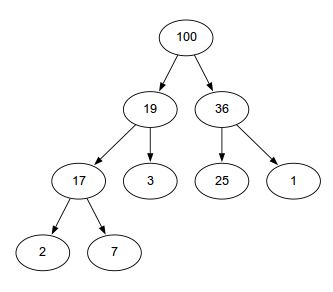
\includegraphics[height=120px,width=120px]{poglavlja/slike/heap.png}
\caption{Zadatak \ref{4_26}}
\label{fig:zadatak426}
\endminipage\hfill
\minipage{0.425\textwidth}
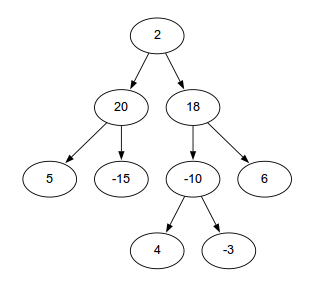
\includegraphics[height=120px,width=120px]{poglavlja/slike/binarna_stabla.png}
\caption{Zadatak \ref{4_27}}
\label{fig:zadatak427}
\endminipage\hfill

\end{figure}

%11.zadatak
%nije resen
\begin{Exercise}[label=4_27]
Dato je binarno stablo celih brojeva.
\begin{enumerate}
\item Napisati funkciju koja pronalazi čvor u stablu sa najvećim zbirom vrednosti iz desnog podstabla.
\item Napisati funkciju koja pronalazi čvor u stablu sa najmanjim zbirom vrednosti iz levog podstabla.
\item Napisati funkciju koja štampa sadržaj svih čvorova stabla na putanji od korena do najdubljeg čvora.
\item Napisati funkciju koja štampa sadržaj svih čvorova stabla na putanji od korena do čvora koji ima najmanju vrednost u stablu.
\end{enumerate}
Napisati program koji testira gore navedene funkcije nad stablom zadatim slikom \ref{fig:zadatak427} i rezultat ispisuje na standardni izlaz.  
%\linkresenje{4_27}

\begin{maxitest}
\begin{test}{1}
#\naslovIzlaz#
#\izlaz{Vrednost u cvoru sa maksimalnim desnim zbirom: 18}#
#\izlaz{Vrednost u cvoru sa minimalnim levim zbirom: 18}#
#\izlaz{2 18 -10 4}#
#\izlaz{2 20 -15}#
\end{test}
\end{maxitest}

\end{Exercise}

%\begin{Answer}[ref=4_27]
%\includecode{resenja/4_DinamickeStrukture/4_27.c}
%\end{Answer}

\section{Rešenja}
\shipoutAnswer

\appendix
\chapter{Ispitni rokovi}

\section{Praktični deo ispita, jun 2015.}

\begin{Exercise}[label=A_01]
Kao argument komandne linije zadaje se ime ulazne datoteke u kojoj se nalaze niske. U prvoj liniji datoteke nalazi se informacija o broju niski, a u narednim linijama po jedna niska ne duža od $50$ karaktera. Napisati program u kojem se dinamički alocira memorija za zadati niz niski, a zatim se na standardni izlaz u redosledu suprotnom od redosleda čitanja ispisuju sve niske koje počinju velikim slovom. U slučaju pojave bilo kakve greške na standardni izlaz za greške ispisati vrednost $-1$ i prekinuti izvršavanje programa.

\begin{miditest}
\begin{test}{1}
#\poziv{./a.out ulaz.txt}#

#\naslovDat{ulaz.txt}#
#\datoteka{5}#
#\datoteka{Programiranje}#
#\datoteka{Matematika}#
#\datoteka{12345}#
#\datoteka{dInAmiCnArEc}#
#\datoteka{Ispit}#
  
#\naslovIzlaz#
#\izlaz{Ispit}#
#\izlaz{Matematika}#
#\izlaz{Programiranje}#
\end{test}
\end{miditest}
\begin{minitest}
\begin{test}{2}
#\poziv{./a.out ulaz.txt}#

#\naslovDat{ulaz.txt}#
#\datoteka{2}#
#\datoteka{maksimalano}#
#\datoteka{poena}#

#\naslovIzlaz#
#\izlaz{}#
\end{test}
\end{minitest}


\begin{miditest}
\begin{test}{3}
#\poziv{./a.out ulaz.txt}#

#\naslovDat{Datoteka ulaz.txt ne postoji}#

#\naslovIzlazZaGresku#
#\izlaz{-1}#
\end{test}
\end{miditest}
\begin{miditest}
\begin{test}{4}
#\poziv{./a.out}#

#\naslovIzlazZaGresku#
#\izlaz{-1}#
\end{test}
\end{miditest}

\linkresenje{A_01}
\end{Exercise}
\begin{Answer}[ref=A_01]
\includecode{resenja/A_IspitniRokovi/A_01.c}
\end{Answer}


\begin{Exercise}[label=A_02]
Data je biblioteka za rad sa binarnim pretraživačkim stablima čiji čvorovi sadrže cele brojeve. 
Napisati funkciju   \kckod{int sumiraj\_n (Cvor * koren, int n)}
koja izračunava zbir svih čvorova koji se nalaze na $n$-tom nivou stabla. Koren se nalazi na nultom nivou, njegova deca na prvom nivou i tako redom. 
Ispravnost napisane funkcije testirati na osnovu zadate  \kckod{main} funkcije i biblioteke za rad sa pretraživačkim stablima.

\noindent Napisati program koji sa standardnog ulaza učitava najpre prirodan broj $n$, a potom i brojeve koje smešta u stablo. Smeštanje brojeva se prekida učitavanjem nule. Zatim se ispisuje rezultat pozivanja funkcije \kckod{sumiraj\_n} za broj $n$ i tako kreirano stablo. U slučaju greške na standardni izlaz za greške ispisati $-1$.
\napomena{Koristiti biblioteku za rad sa binarnim pretraživačkim stablima \ref{4_14}.}

\begin{miditest}
\begin{test}{1}
#\naslovUlaz#
#\ulaz{2 8 10 3 6 14 13 7 4 0}#
#\naslovIzlaz#
#\izlaz{ 20}#
\end{test}
\end{miditest}
\begin{miditest}
\begin{test}{2}
#\naslovUlaz#
#\ulaz{0 50 14 5 2 4 56 8 52 7 1 0}#
#\naslovIzlaz#
#\izlaz{ 50}#
\end{test}
\end{miditest}

\linkresenje{A_02}
\end{Exercise}
\begin{Answer}[ref=A_02]
%\includecode{resenja/A_IspitniRokovi/A_02/stabla.h}
%\includecodeLib{resenja/A_IspitniRokovi/A_02/stabla.h}{stabla.h}
%\includecodeLib{resenja/A_IspitniRokovi/A_02/stabla.c}{stabla.c}
\\
\napomena{Rešenje koristi biblioteku za rad sa binarnim pretraživačkim stablima iz zadatka \ref{4_14}.} 
\includecodeLib{resenja/A_IspitniRokovi/A_02.c}{main.c}
%\includecode{resenja/A_IspitniRokovi/A_02/stabla.c}
%\includecode{resenja/A_IspitniRokovi/A_02/main.c}
\end{Answer}

\begin{Exercise}[label=A_03]
Sa standardnog ulaza učitava se broj vrsta i broj kolona celobrojne matrice $A$, 
a zatim i elementi matrice $A$. Napisati program koji će ispisati indeks kolone u kojoj se nalazi najviše negativnih elemenata. 
Ukoliko postoji više takvih kolona, ispisati indeks prve takve kolone. 
Može se pretpostaviti da je broj vrsta i broj kolona manji od $50$. 
U slučaju greške ispisati vrednost $-1$ na standardni izlaz za greške. 

\begin{minitest}
\begin{test}{1}
#\naslovUlaz#
#\ulaz{4 5}#
#\ulaz{1  2  3  4  5}#
#\ulaz{ -1  2 -3  4 -5 }#
#\ulaz{ -5 -4 -3 -2  1}#
#\ulaz{-1  0  0  0  0 }#
#\naslovIzlaz#
#\izlaz{0}#
\end{test}
\end{minitest}
\begin{minitest}
\begin{test}{2}
#\naslovUlaz#
#\ulaz{2 3}#
#\ulaz{0 0 -5}#
#\ulaz{1 2 -4}#
#\naslovIzlaz#
#\izlaz{2}#
\end{test}
\end{minitest}
\begin{minitest}
\begin{test}{3}
#\naslovUlaz#
#\ulaz{-2}#
#\naslovIzlazZaGresku#
#\izlaz{-1}#
\end{test}
\end{minitest}

\linkresenje{A_03}
\end{Exercise}
\begin{Answer}[ref=A_03]
\includecode{resenja/A_IspitniRokovi/A_03.c}
\end{Answer}

\section{Praktični deo ispita, jul 2015.}

\begin{Exercise}[label=A_04]
Napisati program koji kao prvi arugment komandne linije prima ime dokumenta u kome treba prebrojati sva pojavljivanja tražene niske (bez preklapanja) koja se navodi kao drugi argument komandne linije (iskoristiti funkciju standardne biblioteke \kckod{strstr}). U slučaju
bilo kakve greške ispisati $-1$ na standardni izlaz za greške.
Pretpostaviti da linije datoteke neće biti duže od $127$
karaktera.\\
Potpis funkcije \kckod{strstr}:\\
\kckod{char *strstr(const char *haystack, const char *needle);}\\
Funkcija traži prvo pojavljivanje podniske $needle$ u nisci
$haystack$, i vraća pokazivač na početak podniske, ili
$NULL$ ako podniska nije pronađena.

\skrati{2}
\begin{miditest}
\begin{test}{1}
#\poziv{./a.out ulaz.txt test}#

#\naslovDat{ulaz.txt}#
#\datoteka{ Ovo je test primer. }#
#\datoteka{ U njemu se rec test javlja}#
#\datoteka{vise puta. testtesttest}#

#\naslovIzlaz#
#\izlaz{5}#
\end{test}
\end{miditest}
\begin{miditest}
\begin{test}{2}
#\poziv{./a.out}#

#\naslovIzlazZaGresku#
#\izlaz{-1}# 
\end{test}
\end{miditest}

\begin{miditest}
\begin{test}{3}
#\poziv{./a.out ulaz.txt foo}#

#\naslovDat{Datoteka ulaz.txt ne postoji}#

#\naslovIzlazZaGresku#
#\izlaz{-1}#
\end{test}
\end{miditest}
\begin{miditest}
\begin{test}{4}
#\poziv{ ./a.out ulaz.txt .  }#

#\naslovDat{Datoteka ulaz.txt je prazna}#

#\naslovIzlaz#
#\izlaz{0}#
\end{test}
\end{miditest}

\linkresenje{A_04}
\end{Exercise}
\begin{Answer}[ref=A_04]
\includecode{resenja/A_IspitniRokovi/A_04.c}
\end{Answer}


\skrati{2}
\begin{Exercise}[label=A_05]
Na početku datoteke \kckod{trouglovi.txt} nalazi se broj trouglova čije su koordinate temena zapisane u nastavku datoteke. Napisati
  program koji učitava trouglove i ispisuje ih na standardni izlaz
  sortirane po površini opadajuće. U slučaju bilo kakve greške ispisati $-1$ na standardni izlaz za greške. Ne praviti nikakve pretpostavke o broju trouglova u datoteci i proveriti da li je datoteka ispravno zadata. \uputstvo{Koristiti Heronov obrazac: 
  $P = \sqrt{s*(s-a)*(s-b)*(s-c)}$, gde je $s$ poluobim trougla.}

\skrati{2}
\begin{miditest}
\begin{test}{3}
#\naslovDat{Datoteka trouglovi.txt ne postoji}#

#\naslovIzlazZaGresku#
#\izlaz{-1}#
\end{test}
\end{miditest}
\begin{minitest}
\begin{test}{4}
#\naslovDat{trouglovi.txt}#
#\datoteka{0}#

#\naslovIzlaz#
#\izlaz{}#
\end{test}
\end{minitest}

\begin{miditest}
\begin{test}{1}
#\naslovDat{trouglovi.txt}#
#\datoteka{4}#
#\datoteka{ 0 0 0 1.2 1 0 }#
#\datoteka{ 0.3 0.3 0.5 0.5 0.9 1}#
#\datoteka{-2 0 0 0 0 1}#
#\datoteka{-2 0 0 0 0 1}#

#\naslovIzlaz#
#\izlaz{2 0 2 2 -1 -1}#
#\izlaz{-2 0 0 0 0 1}#
#\izlaz{0 0 0 1.2 1 0}#
#\izlaz{0.3 0.3 0.5 0.5 0.9 1}#
\end{test}
\end{miditest}
\begin{minitest}
\begin{test}{2}
#\naslovDat{trouglovi.txt}#
#\datoteka{3}#
#\datoteka{ 1.2 3.2 1.1 4.3}#

#\naslovIzlazZaGresku#
#\izlaz{-1}#
\end{test}
\end{minitest}


\linkresenje{A_05}
\end{Exercise}

\begin{Answer}[ref=A_05]
\includecode{resenja/A_IspitniRokovi/A_05.c}
\ifpdf \else \newpage \fi
\end{Answer}

\begin{Exercise}[label=A_06]
Data je biblioteka za rad sa binarnim pretraživačkim stablima celih brojeva. Napisati funkciju\\ 
\kckod{int prebroj\_n(Cvor *koren, int n)}\\
  koja u datom stablu prebrojava čvorove na $n$-tom nivou, koji
  imaju tačno jednog potomka. Pretpostaviti da se koren nalazi na
  nivou $0$. Ispravnost napisane funkcije testirati na osnovu zadate
  \kckod{main} funkcije i biblioteke za rad sa stablima. \napomena{Koristiti biblioteku za rad sa binarnim pretraživačkim stablima iz zadatka \ref{4_14}.} 

\skrati{2}
\begin{minitest}
\begin{test}{1}
#\naslovUlaz#
#\ulaz{ 1 5 3 6 1 4 7 9}#
#\naslovIzlaz#
#\izlaz{1}#
\end{test}
\end{minitest}
\begin{minitest}
\begin{test}{2}
#\naslovUlaz#
#\ulaz{2 5 3 6 1 0 4 7 9}#
#\naslovIzlaz#
#\izlaz{2}#
\end{test}
\end{minitest}
\begin{minitest}
\begin{test}{3}
#\naslovUlaz#
#\ulaz{0 4 2 5}#
#\naslovIzlaz#
#\izlaz{0}#
\end{test}
\end{minitest}

\begin{minitest}
\begin{test}{4}
#\naslovUlaz#
#\ulaz{ 3}#
#\naslovIzlaz#
#\izlaz{0}#
\end{test}
\end{minitest}
\begin{minitest}
\begin{test}{5}
#\naslovUlaz#
#\ulaz{-1 4 5 1 7}#
#\naslovIzlaz#
#\izlaz{0}#
\end{test}
\end{minitest}
\skrati{2}

\linkresenje{A_06}
\end{Exercise}
\begin{Answer}[ref=A_06]
%%\includecode{resenja/A_IspitniRokovi/A_06/stabla.h}  
%\includecodeLib{resenja/A_IspitniRokovi/A_06/stabla.h}{stabla.h}
%\includecodeLib{resenja/A_IspitniRokovi/A_06/stabla.c}{stabla.c}
\\
\napomena{Rešenje koristi biblioteku za rad sa binarnim pretraživačkim stablima iz zadatka \ref{4_14}.} 
\includecodeLib{resenja/A_IspitniRokovi/A_06.c}{main.c}
%%\includecode{resenja/A_IspitniRokovi/A_06/stabla.c}
%%\includecode{resenja/A_IspitniRokovi/A_06/main.c}
\end{Answer}

%\ifpdf \else \newpage \fi
\section{Praktični deo ispita, septembar 2015.}

\skrati{2}
\begin{Exercise}[label=A_07]
Sa standardnog ulaza se učitavaju neoznačeni celi brojevi $x$ i $n$. Na
   standardni izlaz ispisati neoznačen ceo broj koji se dobija od broja $x$ kada se njegov binarni zapis
   rotira za $n$ mesta udesno. Na primer, ako je binarni zapis broja $x$ jednak \texttt{00000000000000000000000000001111},
   i ako je $n=1$ tada na standardni izlaz treba ispisati neočnačen broj čiji je binarni zapis jednak \texttt{10000000000000000000000000000111}.

\begin{minitest}
\begin{test}{1}
#\naslovUlaz#
#\ulaz{6 1}#
#\naslovIzlaz#
#\izlaz{3}#
\end{test}
\end{minitest}
\begin{minitest}
\begin{test}{2}
#\naslovUlaz#
#\ulaz{15 3}#
#\naslovIzlaz#
#\izlaz{3758096385}#
\end{test}
\end{minitest}
\begin{minitest}
\begin{test}{3}
#\naslovUlaz#
#\ulaz{31 100}#
#\naslovIzlaz#
#\izlaz{4026531841}#
\end{test}
\end{minitest}

\begin{minitest}
\begin{test}{4}
#\naslovUlaz#
#\ulaz{4 0}#
#\naslovIzlaz#
#\izlaz{4}#
\end{test}
\end{minitest}
\begin{minitest}
\begin{test}{5}
#\naslovUlaz#
#\ulaz{0 5}#
#\naslovIzlaz#
#\izlaz{0}#
\end{test}
\end{minitest}

\linkresenje{A_07}
\end{Exercise}
\begin{Answer}[ref=A_07]
\includecode{resenja/A_IspitniRokovi/A_07.c}
\end{Answer}


\begin{Exercise}[label=A_08]
Data je biblioteka za rad sa listama. Napisati funkciju \kckod{int dopuni\_listu(Cvor ** adresa\_glave)}
koja samo čvorovima koji imaju sledbenika u jednostruko povezanoj listi realnih brojeva,
  dodaje između čvora i njegovog sledbenika nov čvor čija vrednost je aritmetička sredina njihovih vrednosti. Povratna vrednost funkcije treba da bude $1$ ukoliko je došlo greške pri alokaciji memorije, inače $0$.
 Ispravnost napisane funkcije testirati koristeći dostupnu biblioteku za rad sa listama i \kckod{main} funkciju koja najpre
 učitava elemente liste, poziva pomenutu funkciju i ispisuje sadržaj liste.

\begin{maxitest}
\begin{test}{1}
#\naslovUlaz#
#\ulaz{1 2 3 4 5}#
#\naslovIzlaz#
#\izlaz{1.00 1.50 2.00 2.50 3.00 3.50 4.00 4.50 5.00}#
\end{test}
\end{maxitest}

\begin{minitest}
\begin{test}{2}
#\naslovUlaz#
#\ulaz{12}#
#\naslovIzlaz#
#\izlaz{12.00}#
\end{test}
\end{minitest}
\begin{minitest}
\begin{test}{3}
#\naslovUlaz#
#\ulaz{prazna lista}#
#\naslovIzlaz#
#\izlaz{}#
\end{test}
\end{minitest}
\begin{minitest}
\begin{test}{4}
#\naslovUlaz#
#\ulaz{13.3 15.8}#
#\naslovIzlaz#
#\izlaz{13.30 14.55}#
\end{test}
\end{minitest}

\linkresenje{A_08}
\end{Exercise}

\begin{Answer}[ref=A_08]
%\includecode{resenja/A_IspitniRokovi/908/liste.h}
\includecodeLib{resenja/A_IspitniRokovi/A_08/liste.h}{liste.h}
\includecodeLib{resenja/A_IspitniRokovi/A_08/liste.c}{liste.c}
\includecodeLib{resenja/A_IspitniRokovi/A_08/main.c}{main.c}
%\includecode{resenja/A_IspitniRokovi/908/liste.c}
%\includecode{resenja/A_IspitniRokovi/908/main.c}
\ifpdf \else \newpage \fi
\end{Answer}

\begin{Exercise}[label=A_09]
Sa standardnog ulaza se učitava dimenzija $n$ kvadratne celobrojne
    matrice $A$ ($n>0$), a zatim i elementi matrice $A$. Napisati program koji
    proverava da li je data kvadratna matrica magični kvadrat
    (magični kvadrat je kvadratna matrica kod koje su sume brojeva
    u svim redovima i kolonama međusobno jednake). Ukoliko jeste, ispisati na
    standardni izlaz sumu brojeva jedne vrste ili kolone te matrice,
    a ukoliko nije ispisati $-$. Broj vrsta i broj kolona matrice nije
    unapred poznat. U slučaju greške ispisati $-1$ na standardni izlaz za greške. \napomena{Koristiti biblioteku za rad sa celobrojnim matricama iz zadatka \ref{2_19}.}

\begin{minitest}
\begin{test}{1}
#\naslovUlaz#
#\ulaz{4}#
#\ulaz{1 2 3 4}#
#\ulaz{2 1 4 3}#
#\ulaz{3 4 2 1}#
#\ulaz{4 3 1 2}#
#\naslovIzlaz#
#\izlaz{10}#
\end{test}
\end{minitest}
\begin{minitest}
\begin{test}{2}
#\naslovUlaz#
#\ulaz{3}#
#\ulaz{1 1 1}#
#\ulaz{1 1 1}#
#\ulaz{1 1 1}#
#\naslovIzlaz#
#\izlaz{3}#
\end{test}
\end{minitest}
\begin{minitest}
\begin{test}{3}
#\naslovUlaz#
#\ulaz{2}#
#\ulaz{1 1}#
#\ulaz{2 2}#
#\naslovIzlaz#
#\izlaz{-}#
\end{test}
\end{minitest}

\begin{minitest}
\begin{test}{4}
#\naslovUlaz#
#\ulaz{2}#
#\ulaz{1 2}#
#\ulaz{1 2}#
#\naslovIzlaz#
#\izlaz{-}#
\end{test}
\end{minitest}
\begin{minitest}
\begin{test}{5}
#\naslovUlaz#
#\ulaz{1}#
#\ulaz{5}#
#\naslovIzlaz#
#\izlaz{5}#
\end{test}
\end{minitest}
\begin{minitest}
\begin{test}{6}
#\naslovUlaz#
#\ulaz{0}#
#\naslovIzlazZaGresku#
#\izlaz{-1}#
\end{test}
\end{minitest}

\linkresenje{A_09}
\end{Exercise}
\begin{Answer}[ref=A_09]
\includecode{resenja/A_IspitniRokovi/A_09.c}
\end{Answer}

\section{Praktični deo ispita, januar 2016.}
\begin{Exercise}[label=A_10]
Napisati funkciju \kckod{unsigned int zamena(unsigned int x)} koja u datom broju \argf{x} menja mesta prvom i četvrtom bajtu. Prvi bajt je sačinjen od $8$ bitova najmanje težine. Napisati program koji testira funkciju \kckod{zamena} za ceo broj unet sa standardnog ulaza. U slučaju da je uneti broj negativan, na standardni izlaz za greške program ispisuje $-1$, a inače ispisuje na standardni izlaz broj dobijen primenom funkcije \kckod{zamena}. 

\begin{minitest}
\begin{test}{1}
#\naslovUlaz#
#\ulaz{285278344}#
#\naslovIzlaz#
#\izlaz{2281766929}#
\end{test}
\end{minitest}
\begin{minitest}
\begin{test}{2}
#\naslovUlaz#
#\ulaz{1024}#
#\naslovIzlaz#
#\izlaz{1024}#
\end{test}
\end{minitest}
\begin{minitest}
\begin{test}{3}
#\naslovUlaz#
#\ulaz{1}#
#\naslovIzlaz#
#\izlaz{16777216}#
\end{test}
\end{minitest}

\begin{minitest}
\begin{test}{4}
#\naslovUlaz#
#\ulaz{0}#
#\naslovIzlaz#
#\izlaz{0}#
\end{test}
\end{minitest}
\begin{minitest}
\begin{test}{5}
#\naslovUlaz#
#\ulaz{-63}#
#\naslovIzlazZaGresku#
#\izlaz{-1}#
\end{test}
\end{minitest}

\linkresenje{A_10}
\end{Exercise}
\begin{Answer}[ref=A_10]
\includecode{resenja/A_IspitniRokovi/A_10.c}
\end{Answer}


\begin{Exercise}[label=A_11]
Data je biblioteka za rad sa binarnim pretraživackim stablima celih brojeva. Napisati funkciju \kckod{int najduzi\_put (Cvor * koren)} koja za dato stablo izračunava dužinu najdužeg puta od korena do nekog lista. Ako je stablo prazno, povratna vrednost funkcije je $-1$. Ako stablo ima samo koren, dužina najdužeg puta je $0$. Ispravnost napisane funkcije testirati na osnovu zadate \kckod{main} funkcije i biblioteke za rad sa stablima. \napomena{Koristiti biblioteku za rad sa binarnim pretraživačkim stablima celih brojeva iz zadatka  \ref{4_14}.} 

\begin{miditest}
\begin{test}{1}
#\naslovUlaz#
#\ulaz{10 5 15 3 2 4 30 12 14 13}#
#\naslovIzlaz#
#\izlaz{4}#
\end{test}
\end{miditest}
\begin{minitest}
\begin{test}{2}
#\naslovUlaz#
#\ulaz{3}#
#\naslovIzlaz#
#\izlaz{0}#
\end{test}
\end{minitest}

\begin{minitest}
\begin{test}{3}
#\naslovUlaz#
#\ulaz{5 6}#
#\naslovIzlaz#
#\izlaz{1}#
\end{test}
\end{minitest}
\begin{minitest}
\begin{test}{4}
#\naslovUlaz#
#\ulaz{7 5 8}#
#\naslovIzlaz#
#\izlaz{1}#
\end{test}
\end{minitest}
\begin{minitest}
\begin{test}{5}
#\naslovUlaz#
#\ulaz{5 7 8}#
#\naslovIzlaz#
#\izlaz{2}#
\end{test}
\end{minitest}


\linkresenje{A_11}
\end{Exercise}

\begin{Answer}[ref=A_11]
%\includecodeLib{resenja/A_IspitniRokovi/A_08/liste.h}{liste.h}
%\includecodeLib{resenja/A_IspitniRokovi/A_08/liste.c}{liste.c}
\\
\napomena{Rešenje koristi biblioteku za rad sa binarnim pretraživačkim stablima iz zadatka \ref{4_14}.} 
\includecode{resenja/A_IspitniRokovi/A_11.c}
\end{Answer}

\begin{Exercise}[label=A_12]
Sa standardnog ulaza zadaje se ime datoteke u kojoj se nalazi matrica realnih brojeva jednostruke tačnosti
i jedan realan broj. Napisati program koji iz datoteke učitava matricu realnih brojeva, a zatim pronalazi i na standardni
izlaz ispisuje indeks vrste matrice u kojoj se uneti realan broj pojavljuje najmanje puta. Ako postoji više takvih vrsta,
ispisati indeks prve takve vrste. U datoteci su prvo navedena dva cela broja koja predstavljaju dimenzije matrice, redom broj
vrsta i broj kolona, a zatim i elementi matrice vrstu po vrstu. U slučaju greške ispisati $-1$ na standardni izlaz za greške.
Pretpostaviti da ime datoteke neće biti duže od $30$ karaktera. \napomena{U zadatku treba koristiti dinamičku alokaciju memorije.}

\begin{minitest}
\begin{test}{1}
#\naslovUlaz#
#\ulaz{brojevi.txt 0}#

#\naslovDat{brojevi.txt}#
#\datoteka{4 4}#
#\datoteka{0 0 0 1.2}#
#\datoteka{1 0 0.3 0.3}#
#\datoteka{0.5 0.5 0.9 -1}#
#\datoteka{-2 0 0 0}#

#\naslovIzlaz#
#\izlaz{2}#
\end{test}
\end{minitest}
\begin{minitest}
\begin{test}{2}
#\naslovUlaz#
#\ulaz{in.txt 2}#

#\naslovDat{in.txt}#
#\datoteka{3 3}#
#\datoteka{2 0 2}#
#\datoteka{-1 2 -1}#
#\datoteka{2 5 3}#

#\naslovIzlaz#
#\izlaz{1}#
\end{test}
\end{minitest}
\begin{minitest}
\begin{test}{3}
#\naslovUlaz#
#\ulaz{brojevi.txt 12}#

#\naslovDat{Datoteka brojevi.txt je prazna}#

#\naslovIzlazZaGresku#
#\izlaz{-1}#
\end{test}
\end{minitest}

\iffalse
\begin{minitest}
\begin{test}{3}
#\naslovUlaz#
#\ulaz{matrica.txt 7}#

#\naslovDat{matrica.txt}#
#\datoteka{3 2}#
#\datoteka{1.1 -5.31}#
#\datoteka{-3.7 35.24}#
#\datoteka{1.4 2.09}#

#\naslovIzlaz#
#\izlaz{0}#
\end{test}
\end{minitest}
\fi

\linkresenje{A_12}
\end{Exercise}
\begin{Answer}[ref=A_12]
\includecode{resenja/A_IspitniRokovi/A_12.c}
\end{Answer}

\section{Rešenja}
\shipoutAnswer


\end{document}
